\pdftrailerid{}
\pdfinfoomitdate=1
\pdfsuppressptexinfo=15
\input{glyphtounicode}
\pdfgentounicode=1
\pdfgentounicode=1
\pdfglyphtounicode{tfm:lmsy10/mapsto}{007C}
\pdfglyphtounicode{tfm:lmex10/parenleftbig}{0028}
\pdfglyphtounicode{tfm:lmex10/parenrightbig}{0029}
\pdfglyphtounicode{tfm:lmex10/bracketleftbig}{005B}
\pdfglyphtounicode{tfm:lmex10/bracketrightbig}{005D}
\pdfglyphtounicode{tfm:lmex10/vextendsingle}{23D0}
\pdfglyphtounicode{tfm:lmex10/vextenddouble}{2016}
\pdfglyphtounicode{tfm:lmex10/parenleftBig}{0028}
\pdfglyphtounicode{tfm:lmex10/parenrightBig}{0029}
\pdfglyphtounicode{tfm:lmex10/parenleftbigg}{0028}
\pdfglyphtounicode{tfm:lmex10/parenrightbigg}{0029}
\pdfglyphtounicode{tfm:lmex10/parenleftBigg}{0028}
\pdfglyphtounicode{tfm:lmex10/parenrightBigg}{0029}
\pdfglyphtounicode{tfm:lmex10/parenlefttp}{239B}
\pdfglyphtounicode{tfm:lmex10/parenrighttp}{239E}
\pdfglyphtounicode{tfm:lmex10/bracketlefttp}{23A1}
\pdfglyphtounicode{tfm:lmex10/bracketrighttp}{23A4}
\pdfglyphtounicode{tfm:lmex10/bracketleftbt}{23A3}
\pdfglyphtounicode{tfm:lmex10/bracketrightbt}{23A6}
\pdfglyphtounicode{tfm:lmex10/parenleftbt}{239D}
\pdfglyphtounicode{tfm:lmex10/parenrightbt}{23A0}
\pdfglyphtounicode{tfm:lmex10/summationtext}{2211}
\pdfglyphtounicode{tfm:lmex10/summationdisplay}{2211}
\pdfglyphtounicode{tfm:lmex10/productdisplay}{220F}
\pdfglyphtounicode{tfm:lmex10/integraldisplay}{222B}
\pdfglyphtounicode{tfm:lmex10/hatwide}{02C6}
\pdfglyphtounicode{tfm:lmex10/tildewide}{02DC}
\pdfglyphtounicode{tfm:lmex10/bracketleftBig}{005B}
\pdfglyphtounicode{tfm:lmex10/bracketrightBig}{005D}
\pdfglyphtounicode{tfm:lmex10/radicalbig}{221A}
\pdfglyphtounicode{tfm:lmex10/radicalBig}{221A}

\documentclass[11pt]{article}
\usepackage[T1]{fontenc}
\usepackage{lmodern}
\usepackage[margin=1.1in]{geometry}
\usepackage{amsmath,amssymb,amsthm,mathtools,mathrsfs}
\usepackage{microtype,booktabs,array,enumitem}
\usepackage{xcolor,graphicx,tikz}
\usetikzlibrary{arrows.meta,calc,patterns,positioning,decorations.pathreplacing}
\usepackage{hyperref}
\hypersetup{colorlinks=true,linkcolor=blue!45!black,citecolor=green!35!black,urlcolor=blue!55!black,pdftitle={Cardy's formula for critical Poisson--Voronoi percolation},pdfauthor={OpenAI}}
\usepackage[nameinlink,noabbrev,capitalize]{cleveref}
\numberwithin{equation}{section}
\newtheorem{theorem}{Theorem}[section]
\newtheorem{lemma}[theorem]{Lemma}
\newtheorem{proposition}[theorem]{Proposition}
\newtheorem{corollary}[theorem]{Corollary}
\theoremstyle{definition}
\newtheorem{definition}[theorem]{Definition}
\newtheorem{remark}[theorem]{Remark}
\newtheorem{convention}[theorem]{Convention}
\newcommand{\R}{\mathbb R}
\newcommand{\C}{\mathbb C}
\newcommand{\Z}{\mathbb Z}
\newcommand{\N}{\mathbb N}
\newcommand{\PP}{\mathbb P}
\newcommand{\EE}{\mathbb E}
\newcommand{\Peta}{\mathbb P^{\eta}}
\newcommand{\Eeta}{\mathbb E^{\eta}}
\newcommand{\Esp}{\mathbb E_{\mathrm{sp}}}
\newcommand{\eps}{\varepsilon}
\newcommand{\om}{\omega}
\newcommand{\ind}{\mathbf 1}
\newcommand{\dd}{\mathrm d}
\newcommand{\ii}{\mathrm i}
\DeclareMathOperator{\diam}{diam}
\DeclareMathOperator{\dist}{dist}
\DeclareMathOperator{\supp}{supp}
\DeclareMathOperator{\Area}{Area}
\DeclareMathOperator{\Var}{Var}
\DeclareMathOperator{\Rea}{Re}
\DeclareMathOperator{\Ima}{Im}
\setlist{itemsep=3pt,topsep=5pt}
\setlength{\emergencystretch}{1.5em}
\title{Cardy's formula for critical Poisson--Voronoi percolation}
\author{OpenAI}
\date{September 23, 2026}
\begin{document}
\maketitle
\begin{abstract}
We prove Cardy's formula for annealed crossing probabilities in critical
planar Poisson--Voronoi percolation in every bounded Jordan quadrilateral.
This proves the annealed crossing-probability form of the conformal-invariance
conjecture for this model.
\end{abstract}
\tableofcontents
\section{Introduction}\label{sec:introduction}

Cardy's formula predicts that a critical two-dimensional percolation crossing
probability is determined by a conformal parameter of the marked domain
\cite{Cardy1992}. Smirnov proved the formula for site percolation on the
triangular lattice \cite{Smirnov2001}. Schramm's Problem~2.12 asks for the
corresponding conformal-invariance theorem for Voronoi percolation
\cite{Schramm2006}. We prove the annealed Cardy-crossing aspect of this
conjecture for the Poisson model, with no regularity assumption on the
boundary beyond the Jordan property.

\subsection{The crossing law}

Identify the oriented plane with $\C$. For $\eps>0$, let $\eta=X_\eps$ be
a homogeneous Poisson point process of intensity $\eps^{-2}$. For $v\in\eta$
its Voronoi cell is the closed set
\[
 \mathcal V_v=\{z\in\C:|z-v|\le |z-u|\text{ for every }u\in\eta\}.
\]
Independently of $\eta$, color its sites black or white with probability
$1/2$ each, and give each cell the color of its site. Let $\mathcal B_\eps$
be the union of the closed black cells. Probabilities and expectations under
the joint law of the points and colors are denoted by $\PP$ and $\EE$.
Conditional probabilities given the points are denoted by $\Peta$;
$\Esp$ denotes averaging over independent fair colors on a fixed graph.
Thus all probabilities in the main theorem are annealed.

Let $D$ be a bounded Jordan domain and let $a,b,c,d$ be distinct points of
$\partial D$ in counterclockwise order. Boundary arcs always include their
endpoints. Define $\mathcal C_\eps(D;a,b,c,d)$ to be the event that
$\mathcal B_\eps\cap\overline D$ contains a connected subset meeting both
the arc $ab$ and the arc $cd$. The conformal map from $D$ to
$\mathbb H=\{z:\operatorname{Im}z>0\}$ which sends $a,c,d$ to
$0,1,\infty$ extends to the boundary in the sense of Carath\'eodory
\cite[Section~2.1, p.~18]{Pommerenke1992}.
Its value at $b$ is a uniquely determined number $x\in(0,1)$.

\begin{theorem}[Annealed Voronoi crossing law]\label{thm:cardy}
For every bounded Jordan domain $D$ and every four distinct
counterclockwise boundary marks $a,b,c,d$, one has
\begin{equation}\label{eq:cardy}
 \lim_{\eps\downarrow0}\PP\bigl(\mathcal C_\eps(D;a,b,c,d)\bigr)
 =F(x)
 :=\frac{\displaystyle\int_0^x[u(1-u)]^{-2/3}\,\dd u}
          {\displaystyle\int_0^1[u(1-u)]^{-2/3}\,\dd u}
 =\frac{\Gamma(2/3)x^{1/3}}
        {\Gamma(1/3)\Gamma(4/3)}
        {}_2F_1\!\left(\frac13,\frac23;\frac43;x\right).
\end{equation}
\end{theorem}

The theorem resolves positively the annealed Cardy-crossing conjecture
for critical Poisson--Voronoi percolation, the crossing-probability aspect
of Schramm's Problem~2.12 above. Its scope is a limit of crossing
probabilities averaged over geometry and colors. The statement does not
assert convergence of the full interface law or a quenched crossing limit
for arbitrary Jordan domains.
In particular, the result concerns the specified closed-cell crossing
event in every fixed Jordan domain, including domains for which a smooth
boundary approximation alone would not immediately identify that event.

For a fixed rectangle, the established concentration of conditional
crossing probabilities also gives a quenched $L^2$ limit; see
Corollary~\ref{cor:quenched-rectangles} below.

\subsection{Prior work}

The conformal-invariance conjecture for critical crossings developed from
numerical and universality investigations. Langlands, Pouliot and
Saint-Aubin explicitly credit Aizenman with the conformal formulation
\cite[Sections~2.1 and~2.4]{LanglandsPouliotSaintAubin1994}.
Cardy's conformal-field-theory calculation identifies the predicted
crossing function \cite{Cardy1992}. Smirnov's proof on the triangular
lattice uses color-switching identities to construct conformal
observables \cite{Smirnov2001,Smirnov2001Expanded}. Carleson's
representation of Cardy's formula as a linear boundary value in an
equilateral triangle, explained in \cite[Corollary~3]{Smirnov2001Expanded},
also describes the boundary problem at the end of our argument.

The same Cardy function is obtained for critical square-lattice bond
percolation under uniform marked-Jordan approximation
\cite[Theorem~1.2]{OpenAISquareBond2026}.
There the event is an actual open-edge path with all boundary edges
sampled independently and no external connections; here it is an annealed
closed-cell crossing in a fixed Jordan domain. The square-bond theorem
is not used in our proof.

Voronoi percolation provides a random planar geometry whose law has no
preferred lattice direction. Benjamini and Schramm proved a distinct
high-intensity invariance under smooth conformal changes of metric,
with the sampling measure held fixed \cite{BenjaminiSchramm1998}.
Bollob\'as and Riordan established that the critical probability of the
planar Poisson model is $1/2$ \cite{BollobasRiordan2006}.
Uniform box-crossing estimates were established by Tassion \cite{Tassion2016};
quenched crossing estimates were developed by
Ahlberg, Griffiths, Morris and Tassion \cite{AGMT2016}.
Vanneuville's quantitative work supplies comparisons between quenched
and annealed arm probabilities, as well as the crossing estimates used
here \cite{Vanneuville2025}. The conformal-invariance conjecture and its
relation to these partial results are discussed in
\cite[Section~1.2]{Vanneuville2021}. These estimates control crossings and
exceptional geometry; identifying the limiting function requires an
additional argument. Proposition~\ref{prop:probability-input} states the
established estimates at the precise hypotheses used below.

The challenge is to obtain an analytic relation that survives the
irregular embedding. In a related setting, Beffara separates a
color-switching identity from the geometric defect of a non-equilateral
embedding \cite[Sections~3.2--3.3, equations~(13)--(14)]{Beffara2014Mesoscopic}.
His crossing theorem concerns periodic triangulations subdivided into
triangular-lattice pieces, under uniform box-crossing and a specified
relation between the two scales; its limit agrees with triangular-lattice
percolation up to a real-linear transformation determined by the initial
embedding. Here the geometry is Poisson--Delaunay;
we recover the needed relation by transporting exact closed-circuit
identities to open portions of random boundaries.

\subsection{From circuit identities to the crossing law}

The proof begins with the triangular graph joining sites of neighboring
Voronoi cells and its dual graph. Dual edges separating opposite colors
form ordinary cluster-boundary circuits. For each such circuit $L$, we
delete all points of $L$, including its vertices, and retain each
connected component $C$ of the remaining dual graph. An unused edge whose two endpoints lie
on $L$ then leaves an isolated open-edge component. The label is the
pair $(L,C)$, not just the
geometric side of $L$. Except for isolated open-edge components, these
components have simple monochromatic primal boundaries $P$, called
\emph{rims}, oriented with their component on the left. Keeping the full
component label, including isolated edges, is what makes the exact
orthogonality identity of Section~\ref{sec:fields} hold.

Each triangle is the image of a reference equilateral triangle under
an orientation-preserving real-affine map. The complex-linear and
antilinear parts of this map split each clockwise side vector into two
terms. For a smooth test function $f$, take the contributions for the
side belonging to $P$ in each triangle immediately to its right, and
weight them by $f$ at the triangle's barycenter. Summing the complex-linear
terms gives $U_P(f)$; summing the antilinear terms gives $Q_P(f)$.
Thus $Q$ records the departure from equilateral geometry, while
$V_P(f)=U_P(f)+Q_P(f)$ is the weighted tangent displacement. Orthogonality gives a separate exact second-moment
identity for each Fourier field when summed over all component labels,
including isolated open edges.
The complete tangent sum is $V_P(1)=0$ on every closed rim.
Stationarity makes the corresponding macroscopic closed-rim sums of $Q$
small. The main task is to open that identity: along a common microscopic
subsequence, we prove
\[
                    Q_P(f)-aV_P(f)\longrightarrow0
\]
in probability, uniformly over rims extending beyond a fixed collar of
$\supp f$. The scalar $a$ is independent of the later test and bulk patch;
Theorem~\ref{thm:bulk-transport} states the precise local formulation.

For this passage to open arcs, we retain local colored configurations near
endpoints in deterministic regions called \emph{plugs}. Separated
two-color corridors join them into closed experiments. Surrounding circuits restrict the path to the same two contacts, and the
absence of an alternative monochromatic path on its right forces agreement
when the exterior configuration is changed. For each fixed connector, conditional resampling produces a function of
the two endpoint states, common to its completions, whose sum around each
fixed cycle is small.
Comparing closures and inserting intermediate plugs decomposes this
function into an affine displacement, two local endpoint potentials, and
a controlled remainder. Sections~\ref{sec:plugs} and~\ref{sec:affine}
construct this endpoint transport before it is used on a random arc.

Two issues remain in returning to actual rims. The local geometry and
colors have already selected the arc, so the comparison must retain their
conditioning. At each fixed comparison scale, arm estimates provide a
finite menu of plug models densely along every relevant rim and a finite
deterministic family of connecting patterns. The comparison is made with
unnormalized subprobabilities dominated by the original law; there is no
division by a configuration-dependent fitting probability. A second issue
is cancellation: the fields are signed, so a small change in their
coefficients is not controlled by a path-length estimate. Deterministic
spatial refinement, a near-return bound, and the orthogonality identity
supply that control. Sections~\ref{sec:pins} and~\ref{sec:actual-arcs}
complete these two steps in the order needed for bulk transport.

The final steps prove $1-2\operatorname{Re}a>0$ for the scalar $a$
appearing in the transport relation. In particular, the coefficient
$1-a$ needed by the observable is nonzero. Complete a finite discrete
disk by three exterior marked vertices; a component observable at this
closing triangle records which boundary connection occurs. One of its
boundary coefficients is exactly the crossing probability. Orthogonality
and the transport relation give the contour cancellation needed for a
holomorphic limit. The scalar $a$ need not be identified: once
$1-a\ne0$, it disappears from the limiting Cauchy--Riemann equation.
The resulting boundary-value problem has the conformal map to an
equilateral triangle as its unique solution
(Propositions~\ref{prop:observable} and~\ref{prop:holomorphy}, and
Lemma~\ref{lemma:boundary-uniqueness}). This common boundary problem
identifies every subsequential crossing limit.
A deterministic comparison at fixed buffers in a Schoenflies chart then
transfers this crossing law to the exact closed-cell event in arbitrary
Jordan domains.

\subsection{A quenched consequence for rectangles}

\begin{corollary}[Quenched Cardy limit for fixed rectangles]\label{cor:quenched-rectangles}
Let $D$ be a fixed bounded nondegenerate open rectangle and let $a,b,c,d$
be its corners in counterclockwise order, with $ab$ and $cd$ the chosen
opposite sides. Write $x_D$ for its conformal parameter above and set
\[
 Q_\eps(\eta)=\Peta\bigl(\mathcal C_\eps(D;a,b,c,d)\bigr),
 \qquad \eta=X_\eps.
\]
If $\PP_{\mathrm{geom},\eps}$ and $\EE_{\mathrm{geom},\eps}$ denote
probability and expectation for the Poisson geometry at mesh $\eps$, then
\[
 \lim_{\eps\downarrow0}
 \EE_{\mathrm{geom},\eps}\bigl[|Q_\eps-F(x_D)|^2\bigr]=0.
\]
In particular, for every $t>0$,
$\PP_{\mathrm{geom},\eps}(|Q_\eps-F(x_D)|>t)\to0$.
These limits use the geometry law at each mesh, without a coupling across
meshes.
\end{corollary}

\begin{proof}
Almost surely only finitely many Voronoi cells meet $\overline D$, and
each cell clipped to $\overline D$ is closed and convex. Every connected
component of a finite union of such clipped cells is path connected, by
concatenating segments through a chain of intersecting cells. Thus, almost
surely in the geometry and for every coloring, our connected-set crossing
event agrees with the continuous closed-cell crossing event in
\cite[Definition~1.1]{Vanneuville2025}.

After an orientation-preserving isometry, write
$\overline D=[-w,w]\times[-h,h]$, with the chosen sides vertical.
Scaling by $\eps^{-1}$ sends the full-plane intensity-$\eps^{-2}$ Poisson
process to unit intensity and this rectangle to
$[-\lambda R,\lambda R]\times[-R,R]$, where $\lambda=w/h$ and
$R=h/\eps$. The Voronoi cells and their conditional fair coloring
commute with this similarity. Therefore
\cite[Theorem~1.3]{Vanneuville2025} gives an absolute $\alpha>0$ and a
constant $C_\lambda<\infty$ such that, for $0<\eps\le h$,
\[
 \Var_{\mathrm{geom},\eps}(Q_\eps)
 \le C_\lambda(\eps/h)^\alpha.
\]
Let $m_\eps=\PP(\mathcal C_\eps(D;a,b,c,d))$. Conditioning on the
geometry gives $\EE_{\mathrm{geom},\eps}Q_\eps=m_\eps$, while
Theorem~\ref{thm:cardy} gives $m_\eps\to F(x_D)$. Hence
\[
 \EE_{\mathrm{geom},\eps}|Q_\eps-F(x_D)|^2
 =\Var_{\mathrm{geom},\eps}(Q_\eps)+|m_\eps-F(x_D)|^2
 \le C_\lambda(\eps/h)^\alpha+|m_\eps-F(x_D)|^2
 \longrightarrow0.
\]
Markov's inequality gives the assertion in probability.
\end{proof}

\subsection{Geometry, bulk patches and notation}

Write $\omega=\exp(2\pi\ii/3)$. Unless specified otherwise, sites, edges
and triangles belong to the primal Delaunay triangulation. Either
color can be the path color; we describe it as black when making a
construction. Distances, diameters and balls are Euclidean, and complex
vectors use the positive orientation of the plane.

We recall the geometric facts behind this convention. Almost surely,
the Poisson process is locally finite and has neither collinear triples
nor cocircular quadruples, by diffuseness and a countable exhaustion.
For a finite set in general position, empty-circumdisk triangles form
the triangulation of its convex hull: lift the sites to the paraboloid
and project the lower faces. Their circumcenters are Voronoi vertices,
and shared cell sides correspond to primal edges. The local
determination estimate in Lemma~\ref{lemma:mesh} makes these finite
constructions stabilize on every compact set along an exhaustion.
It also bounds the cells of sites in any fixed compact set. Thus the
full-plane cells form a locally finite polygonal tiling with trivalent
meeting points. Sites of touching cells are primal neighbors, including
when the cells meet at a vertex. The primal graph can equivalently be
drawn through the tiling by joining sites to interior points of shared
cell sides. This drawing has the same planar orders as the straight
Delaunay drawing.

\begin{definition}[Bulk setting]\label{def:bulk-setting}
A bulk setting is either the full-plane sample or a finite simple
triangulation of the sphere carrying independent fair site colors
conditional on its graph and geometry. In the latter case an oriented
open planar patch is coupled to a full-plane sample so that, on every
fixed compact subset of the patch, the graphs and their colors agree
with probability tending to one as $\eps\downarrow0$. The graph and
chart agreement event is independent of color sampling conditional on
the geometry. Spatial weights are used only on triangles in the
agreement patch. Compactly supported tests may be set to zero on the
exceptional geometry event.
\end{definition}

The finite completions will be useful when the observable is formed
near the boundary. No geometric control of their triangles outside
the patch is required for the local field identities.

We use the Jordan--Schoenflies theorem in its prescribed-boundary form
\cite[Theorem~10.4]{Moise1977}, its extension to a simple planar arc
\cite[Premi\`ere Partie, Chapitre~I, Section~17]{Antoine1921},
and Carath\'eodory's boundary extension theorem. We also use
the following form of the Rad\'o convergence theorem
\cite[Section~1, pp.~182--183]{Rado1923}. If Jordan
boundaries have parametrizations converging uniformly and in order to
a Jordan boundary, their Riemann maps, normalized at a common interior
point and with positive derivative, converge uniformly in the
closed-disk parametrization to the limiting chart. When a prescribed
ordered cut is to be realized by an ambient change, we give the
extension argument explicitly in Lemma~\ref{lemma:exact-fit}.
Paths, band sides and gates are always considered together with their
planar embeddings.

\subsection{Reading the proof and the order of limits}

Section~\ref{sec:fields} establishes the exact fields and the stationary
closed-sum estimate. Section~\ref{sec:probability} states the percolation
inputs and derives the local arm and mesh estimates.
Sections~\ref{sec:plugs} and~\ref{sec:affine} construct the state
transport and its affine decomposition. Sections~\ref{sec:pins}
and~\ref{sec:actual-arcs} place plugs on actual rims and prove the bulk
transport theorem. Section~\ref{sec:nondegeneracy} excludes its
degenerate scalar. Section~\ref{sec:observable} constructs the
holomorphic limit and proves Theorem~\ref{thm:cardy}.

Throughout the transport construction, the microscopic limit
$\eps\downarrow0$ is taken first, at a fixed comparison scale $h$ and
for finitely many fixed patterns. Pattern-specific positive
conditioning probabilities may be small. Bounds asserted to be
uniform of order $h$ use only a fixed finite family of short normalized
templates. Spatial refinement depth is also fixed during the
microscopic limit and is subsequently increased before $h$ decreases.
The final Jordan-domain buffers are fixed until the microscopic
crossing limit has been taken. Each argument below specifies which of
these limits is in use.

\section{Circuit components and orthogonal fields}\label{sec:fields}

The finite identity in this section is independent of the geometry of a
triangulation.  Geometry enters only when we assign displacement vectors to
its sides.  A component beside a dual circuit, rather than the whole side of
that circuit, is the coordinate of the identity. We first obtain the
separate second-moment identities for the two displacement fields and
then use stationarity to control their complete macroscopic rim sums.

\subsection{An exact identity on a triangulated sphere}

Fix a finite simple triangulation $T$ of the oriented sphere, and give its
vertices independent fair colors.  Draw its trivalent dual $\Gamma$ through
the interiors of the triangles.  A dual edge is \emph{occupied} when the
endpoints of the primal edge it crosses have different colors.  At a dual
vertex there are either zero or two occupied edges.  The occupied subgraph
is therefore a union of vertex-disjoint simple circuits.

In fact its law is uniform on the even subgraphs of $\Gamma$.  To see this,
prescribe a set of primal edges across which the spin changes.  Spins can be
recovered, starting from one vertex, precisely when the number of prescribed
changes around every primal cycle is even.  The face boundaries generate the
cycle space of a spherical triangulation, so it is enough to check the
triangular faces.  These are exactly the even-degree conditions in the dual.
Every allowable prescription has the two spin assignments obtained from one
another by interchanging the colors.

For each occupied circuit $L$, take the connected components $C$ of the
topological graph $\Gamma\setminus L$: all points of $L$, including its
vertices, are removed.  In particular, an open edge whose two endpoints have
been removed can be a component by itself.  Figure~\ref{fig:component-labels}
illustrates the deletion convention in the tetrahedral dual.
Put $\lambda=(L,C)$ and, for a
point $m$ in the interior of a dual edge, define
\[
 H_\lambda(m)=\ind_{\{m\in C\}}.
\]
Vectors indexed by these pairs, with the index set taken separately in each
configuration, have the scalar product
\[
 \langle F,G\rangle
   =\Esp\sum_\lambda F_\lambda\overline{G_\lambda}.
\]
Here and throughout the finite discussion, $\Esp$ averages colors with the
triangulation fixed.  Write $H(m)=(H_\lambda(m))_\lambda$ and
$K(m,n)=\langle H(m),H(n)\rangle$.

\begin{figure}[tbp]
\centering
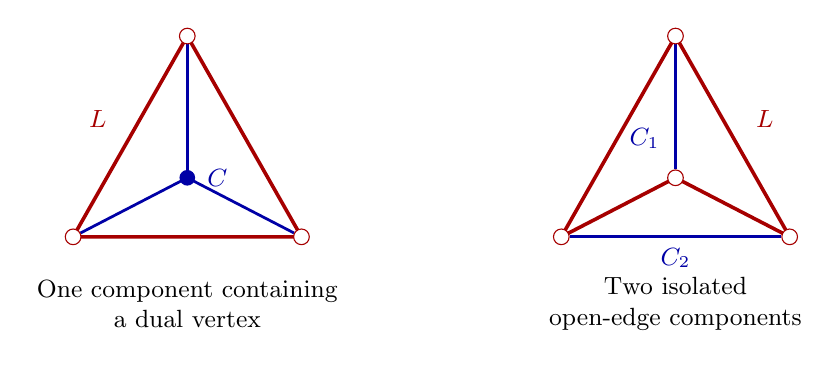
\begin{tikzpicture}[
  wall/.style={red!65!black,line width=1.3pt},
  component/.style={blue!65!black,line width=1pt,shorten <=3pt,shorten >=3pt},
  deleted/.style={circle,draw=red!65!black,fill=white,inner sep=2pt},
  retained/.style={circle,fill=blue!65!black,inner sep=2pt},
  every node/.style={font=\small}]
\begin{scope}[xshift=-3.1cm]
  \coordinate (a) at (0,1.55);
  \coordinate (b) at (-1.45,-1);
  \coordinate (c) at (1.45,-1);
  \coordinate (d) at (0,-.25);
  \draw[wall] (a)--(b)--(c)--cycle;
  \draw[component,shorten >=0pt] (a)--(d);
  \draw[component,shorten >=0pt] (b)--(d);
  \draw[component,shorten >=0pt] (c)--(d);
  \foreach \v in {a,b,c} \node[deleted] at (\v) {};
  \node[retained] at (d) {};
  \node[blue!65!black,right] at (.13,-.25) {$C$};
  \node[red!65!black,left] at (-.9,.5) {$L$};
  \node[align=center] at (0,-1.85)
    {One component containing\\a dual vertex};
\end{scope}
\begin{scope}[xshift=3.1cm]
  \coordinate (a) at (0,1.55);
  \coordinate (b) at (-1.45,-1);
  \coordinate (c) at (1.45,-1);
  \coordinate (d) at (0,-.25);
  \draw[wall] (a)--(b)--(d)--(c)--cycle;
  \draw[component] (a)--(d);
  \draw[component] (b)--(c);
  \foreach \v in {a,b,c,d} \node[deleted] at (\v) {};
  \node[blue!65!black,left] at (-.08,.25) {$C_1$};
  \node[blue!65!black,below] at (0,-1.02) {$C_2$};
  \node[red!65!black,right] at (.9,.5) {$L$};
  \node[align=center] at (0,-1.85)
    {Two isolated\\open-edge components};
\end{scope}
\end{tikzpicture}
\caption{Components in the tetrahedral dual $\Gamma=K_4$.
The heavy red circuit $L$ and its hollow vertices are shown for reference
but are deleted. The remaining blue graph has one component in the left
panel and two in the right panel; its endpoints at deleted vertices are excluded.
Components are determined by connectivity in $\Gamma\setminus L$.}
\label{fig:component-labels}
\end{figure}

\begin{lemma}[Two defects]\label{fields:defects}
For distinct edge-interior points $m,n$, subdivide the dual edges at these
points and take a uniform subgraph with odd degree at $m,n$ and even degree
elsewhere.  Then $K(m,n)$ is the expected number of circuits in this
subgraph.  The assertion also applies to distinct points on the same edge.
\end{lemma}

\begin{proof}
For any even set $D$ of vertices of a connected finite graph, the subgraphs
with boundary $D$, when nonempty, form an affine translate of the cycle
space.  Toggling a path between two prescribed defects gives such a
translation.  In particular, the even and two-defect ensembles have the same
cardinality; subdividing an edge does not change that cardinality.

In the present two-defect ensemble, ordinary vertices have occupied degree
zero or two, while the degree-two marked vertices have occupied degree one.
Thus there is one simple defect path and a collection of disjoint circuits.
Fix a possible circuit $L$.  When it is occupied, every third edge at a
vertex of $L$ is unoccupied.  A defect path must consequently lie in
$\Gamma\setminus L$.  The circuit can occur in the defect ensemble only if
$m,n$ lie in the same component of this complement.  If they do, fix a path
between them in that component.  Toggling it bijects even subgraphs
containing $L$ with two-defect subgraphs containing $L$.  Hence
\[
 \PP_{m,n}(L\text{ occupied})
 =\PP_{\varnothing}(L\text{ occupied})
   \ind_{\{m,n\text{ in one component of }\Gamma\setminus L\}}.
\]
Summing over $L$ proves the assertion.  If the two marks lie on one edge,
its open interior connects them whenever that edge is not in $L$, even when
both endpoints of the edge belong to $L$.
\end{proof}

At a dual vertex corresponding to a triangle $t$, choose points
$m_j(t)$ on its three spokes, indexed by $j=0,1,2$ in positive cyclic order.
Choose the star neighborhoods disjoint.  With
$\om=\exp(2\pi\ii/3)$, set
\[
 Z_t=\sum_{j=0}^2\om^jH(m_j(t)).
\]

\begin{proposition}[Finite orthogonality]\label{fields:orthogonality-prop}
For distinct triangles $t,u$,
\begin{equation}\label{fields:orthogonal}
 \langle Z_t,Z_u\rangle=0,
 \qquad \|Z_t\|^2=\frac34.
\end{equation}
\end{proposition}

\begin{proof}
For the off-diagonal identity, start with uniform oddness at the two dual
vertices $t,u$.  Toggle the short segment from $t$ to $m_j(t)$ and that from
$u$ to $m_k(u)$.  This moves the defects to the two marked points and
preserves uniformity.  By \cref{fields:defects}, it suffices to take the
$\sum_{j,k}\om^{j-k}$ Fourier sum of the resulting circuit counts.

Delete the interiors of the two small stars.  For a fixed initial
configuration, what remains consists of circuits and paths pairing its
occupied star ports.  Each star has either one or three such ports.  The
outside circuits contribute a constant.  If a star has one occupied port,
the modified defect path uses that port regardless of which short segment
was toggled, so the circuit count is independent of that star's index.
These terms vanish in the Fourier sum.

It remains to consider three occupied ports at each star.  There are two
possibilities.  With one through path, the two other ports at each star are
paired by an outside cap.  If $r_t,r_u$ are the through ports, the additional
circuit count after moving the defects is
\[
 \ind_{\{j=r_t\}}+\ind_{\{k=r_u\}}.
\]
It is a sum of one-index terms and again has zero double Fourier sum.  With
three through paths, let $\pi$ be their matching of ports.  An additional
circuit is formed exactly when $k=\pi(j)$: the other two through paths then
join into one circuit.  Disjoint paths between the two boundary circles of
the punctured sphere reverse their positive cyclic orders, so
$\pi(j)=\ell-j\pmod 3$ for some $\ell$.  Their contribution is
\[
 \sum_{j=0}^2\om^{j-\pi(j)}
   =\om^{-\ell}\sum_{j=0}^2\om^{2j}=0.
\]
This establishes the cancellation for each initial configuration, including
when $t,u$ are adjacent.

For the norm, a circuit avoiding $t$ places the three nearby spoke points in
one component, whose Fourier sum is zero.  If $t$ is occupied, exactly one
circuit passes through it.  The two used spokes belong to that circuit,
while the missing spoke belongs to exactly one complementary component.
Thus $Z_t$ has precisely one nonzero coordinate, of modulus one, in this
case.  The three distinct primal vertices of $t$ are not all the same color
with probability $3/4$, proving the second identity.  Equivalently, any
diagonal kernel in this calculation can be evaluated using two distinct
points of the same spoke, which have identical $H$-vectors; coincident
defects are never needed.
\end{proof}

\subsection{The two displacement fields}

Suppose $t$ is drawn as a straight triangle in an oriented plane chart.
Let $z_t$ be its barycenter, and let $d_{tj}$ be the complex side vector
dual to spoke $j$, traversed clockwise around $t$.  Since the three side
vectors sum to zero, there are unique $p_t,q_t\in\C$ such that
\begin{equation}\label{fields:side-decomposition}
 d_{tj}=p_t\om^j+q_t\overline{\om}^{j},
 \qquad
 p_t=\frac13\sum_jd_{tj}\om^{-j},
 \quad q_t=\frac13\sum_jd_{tj}\om^j.
\end{equation}
Applying the real affine map from an equilateral triangle to $t$ gives
\begin{equation}\label{fields:area}
 |p_t|^2-|q_t|^2=\frac4{\sqrt3}\Area(t),
 \qquad |p_t|+|q_t|\le C\diam(t).
\end{equation}
Indeed the two Fourier coefficients are the complex-linear and
antilinear parts of this map, whose Jacobian is their squared-modulus
difference; the equilateral case fixes the constant and sign.

A triangle $t$ is \emph{tagged} for $\lambda=(L,C)$ by $j$ if $L$ uses $t$
and its missing spoke $j$ belongs to $C$.  For a coefficient function $g$
supported where the side vectors are defined, put
\begin{align*}
 U_\lambda(g)&=\sum_{t\text{ tagged by }j}g(z_t)p_t\om^j,\\
 Q_\lambda(g)&=\sum_{t\text{ tagged by }j}g(z_t)q_t\overline{\om}^{j},
 &V_\lambda(g)&=U_\lambda(g)+Q_\lambda(g).
\end{align*}
Changing the first spoke index changes the Fourier coefficients by the
inverse phases, so the summands are well defined.  A rotation of the chart
multiplies each of the two summands by the corresponding complex rotation.

The $\lambda$-coordinate of $Z_t$ is exactly $\om^j$ when $t$ has that tag,
and is zero otherwise.  Its conjugate gives the other phase.  Consequently
\cref{fields:orthogonal} gives the exact identities
\begin{equation}\label{fields:energy}
 \Esp\sum_\lambda |Q_\lambda(g)|^2
   =\frac34\sum_t|g(z_t)q_t|^2,
 \qquad
 \Esp\sum_\lambda |U_\lambda(g)|^2
   =\frac34\sum_t|g(z_t)p_t|^2.
\end{equation}
In particular,
\begin{equation}\label{fields:V-energy}
 \Esp\sum_\lambda |V_\lambda(g)|^2
 \le \frac32\sum_t|g(z_t)|^2\bigl(|p_t|^2+|q_t|^2\bigr).
\end{equation}
We call these the \emph{Bessel bounds}.  The coefficients may be arbitrary
complex numbers depending on the graph and its geometry, but must be
independent of its colors.  Continuity is not required.  In particular,
these bounds apply to deterministic spatial masks.  The sums include every
component, including isolated open edges.

\subsection{Rims and their extremality}

\begin{lemma}[Component rims]\label{lemma:rim}
If $C$ contains a dual vertex, the union of the closed primal triangles
whose centers belong to $C$ has one simple monochromatic boundary circuit
$P$.  Orient $P$ with $C$ on its left.  Its right-hand triangles are exactly
the tags of $(L,C)$, one per edge, and their facing third vertices belong to
one cluster of the opposite color.  The oriented circuit $P$ determines
$(L,C)$.

If $C$ contains no dual vertex, it is an isolated open edge.  It has exactly
two tags.  When they are in one plane chart, their contributions satisfy
\begin{equation}\label{fields:isolated}
 V_{(L,C)}(g)=\bigl(g(z_t)-g(z_u)\bigr)d_{te},
 \qquad V_{(L,C)}(1)=0,
\end{equation}
where $t,u$ are its endpoint triangles and $e$ their common missing side.
\end{lemma}

\begin{proof}
The triangles with centers in $C$ are connected through shared sides.
A boundary side separates such a triangle from a triangle visited by $L$;
the latter's missing spoke leads into $C$.  This identifies the boundary
sides with the tags.

At a primal vertex, the sectors belonging to $C$ form one cyclic interval,
unless they fill its entire neighborhood.  Otherwise choose two separated
runs of $C$-sectors.  Each intervening interval contains an $L$-sector: an
immediately adjacent untouched triangle would still connect to $C$.
Extend two selected $C$-sectors and two intervening $L$-sectors to alternating
points of a sufficiently small circle about the primal vertex, using short
segments inside the sectors.  Outside that circle they are joined in the
two disjoint connected sets $C$ and $L$.  Two disjoint connected sets in
the complementary disk cannot join alternating boundary contacts, a
contradiction.

It follows that the union of the closed $C$-triangles is a connected
subsurface of the sphere with disjoint simple boundary circuits.  Each
boundary circuit faces a different complementary disk.  The connected
circuit $L$ avoids this subsurface and faces it across every boundary side,
so there can be only one such disk and one boundary circuit.  This is $P$.
The missing side at an occupied triangle has equal-colored endpoints;
hence all vertices of $P$ have the same color.  Following either side of a
disagreement circuit gives a connected walk of constant color: within a
visited triangle the adjacent site either stays the same or changes across
an edge joining two sites of that color.  The vertices facing $P$ therefore
lie in one opposing cluster.

Any directed edge of $P$ identifies its occupied right triangle and thus
$L$; its left triangle identifies $C$.  Finally, a component with no dual
vertex must be one open edge with both endpoints on $L$.  Those endpoints
give its two tags, whose side vectors are opposite.  This proves
\eqref{fields:isolated}.  Their separate $U$- and $Q$-contributions need not
vanish.
\end{proof}

We call $P$ an oriented \emph{rim} and write $U_P,Q_P,V_P$ for the
corresponding fields.  If its entire drawing is in plane coordinates,
$V_P(1)$ is the sum of its oriented edge displacements, and hence is zero.
Restricting \eqref{fields:energy} to genuine rims gives inequalities; the
equalities themselves retain the isolated components.

\begin{lemma}[No right bypass and its converse]\label{lemma:no-bypass}
A rim has no path of its own color joining two distinct rim vertices with
all its other points in the open right-hand disk.  Conversely, a simple
monochromatic circuit with this property, and with an opposite-colored site
in its right-hand disk, is a rim.
\end{lemma}

\begin{proof}
An alleged bypass may be made simple.  It is a crosscut of the right-hand
disk and separates its two nonempty rim arcs.  Choose an edge on each arc.
Its facing triangle lies on that arc's side of the crosscut, since a
primal graph path cannot cross the interior of a face.  Its opposing
vertex does not lie on the bypass.  Thus the two facing vertices are in
different parts of the cut disk.  Their opposing cluster can cross neither
the monochromatic rim nor the monochromatic bypass, contradicting
\cref{lemma:rim}.

For the converse, let $uv$ be an edge of the given circuit and $w$ the third
vertex of its right triangle.  If $w$ had the circuit color and lay strictly
on the right, $u,w,v$ would be a bypass.  If $w$ belonged to the circuit,
one of $uw,wv$ would be a right-side chord, unless the right disk were that
single triangular face.  The latter possibility has no opposite-colored
site and is excluded by hypothesis.  Every facing vertex is therefore of
the opposite color.

Choose the occupied dual circuit $L$ through one facing triangle.  It
cannot cross the monochromatic circuit, so it stays on its right.  The
triangles on the left are untouched and form part of one component $C$
off $L$.  Its rim $P^*$ includes the chosen edge and lies in the closed
right side of the original circuit, since its left subsurface contains
the original left disk.  If the two circuits differed, a segment of $P^*$
between successive contacts with the original circuit would be a right
bypass.  Such a segment has distinct endpoints by simplicity: follow
$P^*$ from the common edge to its first departure and then to its next
contact.  This contradicts the hypothesis, proving equality.
\end{proof}

\begin{lemma}[Sandwich]\label{lemma:sandwich}
In an annular band, suppose that there are disjoint essential simple black
and white circuits, with the white circuit on the right of the black one
for the direction of the band.  There is a black rim, with this direction,
in the closed region between them.
\end{lemma}

\begin{proof}
Take a maximal biconnected block of the black graph containing the given
black circuit.  The face of this block toward the white circuit has a
simple boundary.  That boundary lies between the two given circuits:
the block contains the black one and cannot cross the white one.  A black
bypass in this face would add an ear between two distinct vertices of the
block and enlarge the block, contrary to maximality.  The white circuit
supplies an opposite-colored site in the face.  Apply
\cref{lemma:no-bypass}.  In the full plane the same argument uses the finite
black cluster containing the given circuit.
\end{proof}

\subsection{Infinite volume and closed sums}

The local estimates of \cref{sec:probability} imply the following facts
for Poisson--Voronoi percolation.  There are almost surely no infinite
monochromatic clusters: the one-arm bound tends to zero as the outer
radius tends to infinity, and a countable collection of inner boxes covers
the plane.  An infinite disagreement wall would have infinite connected
site chains on both its sides, so every occupied wall is finite as well.

The dual graph has one end.  Indeed, enclose any finite removed part and
all its incident triangles in a compact set.  Plane paths outside a larger
compact set, avoiding primal vertices, connect sufficiently remote
triangles by face adjacency without meeting the removed part.  All such
triangles are therefore in one component.  This observation also shows
that, for a fixed finite circuit $L$, component relations among finitely
many points off $L$ stabilize in sufficiently large spherical completions.

By \cref{lemma:mesh}, increasing simple primal cycles can be chosen around
any fixed compact set.  Keep their interiors and triangulate the outside
to obtain finite simple spherical triangulations, with independent fair
colors on the additional vertices and the original colors inside.  For
any fixed finite set of triangles, their occupied walls eventually agree
with the full-plane walls, and the preceding component relations agree.
The bounded quantities
\[
 \sum_\lambda Z_{t,\lambda}\overline{Z_{u,\lambda}}
\]
therefore converge.  Conditional on almost every point configuration this
holds with color probability one, by the absence of infinite clusters and
Fubini's theorem.  Passing to the limit proves
\eqref{fields:orthogonal}--\eqref{fields:V-energy} for finite local tests
in the full plane, and then for their square-summable limits.  This uses
only local tag products, not finiteness of the norm of an individual
infinite-volume vector $H(m)$.  The same identities hold in any bulk patch
of a spherical completion, for weights supported where its geometry is
defined.  The rim statements follow either by this exhaustion or by
compactifying the plane around a finite wall.

\begin{proposition}[Closed-sum tail]\label{fields:closed-prop}
For every fixed bounded box $B\subset\C$ and every $a>0$, the full-plane
model of spacing $\eps$ satisfies
\begin{equation}\label{fields:closed}
 \lim_{\eps\downarrow0}
 \EE\!\sum_{\substack{P\text{ a rim},\ P\subset B\\\diam(P)\ge a}}
                   |Q_P(1)|^2=0.
\end{equation}
The corresponding full sums for $V_P$ vanish identically.
\end{proposition}

\begin{proof}
Work first at spacing one.  Anchor each rim at the average of its vertex
positions, denoted $b(P)$.  This choice is translation equivariant.  For
$s>0$, retain only those rims all of whose tagged barycenters are within
distance $s$ of their anchor, and define the stationary random measure
\[
 \mu_s=\sum_{P\text{ retained}}|Q_P(1)|^2\delta_{b(P)}.
\]
For anchors in a square $W_R$ of side $R$, the full sum of every retained
rim equals its sum against $\ind_{W_R^{+s}}$, where $W_R^{+s}$ is the
$s$-neighborhood of the square.  Thus \eqref{fields:energy} and stationarity
give
\[
 \EE\mu_s(W_R)
 \le \frac34\EE\sum_{z_t\in W_R^{+s}}|q_t|^2
 =c_q\Area(W_R^{+s}).
\]
The finite constant $c_q$ exists by \cref{lemma:mesh}.  Dividing by $R^2$
and letting $R$ grow shows that the intensity of $\mu_s$ is at most $c_q$,
uniformly in $s$.  Every rim has finitely many tags, so monotone convergence
gives a finite intensity for
\[
 \mu=\sum_P|Q_P(1)|^2\delta_{b(P)}.
\]
Let $\theta(M)$ be the intensity restricted to rims of diameter at least
$M$.  Since each rim is finite and $\mu$ has finite mean on a unit square,
$\theta(M)\to0$ as $M\to\infty$.

Rescaling a spacing-one configuration by $\eps$ multiplies each $Q$ sum
by $\eps$ and anchor area by $\eps^2$.  Consequently, the expected squared
mass of spacing-$\eps$ rims of diameter at least $a$, with anchors in $B$,
is $\Area(B)\theta(a/\eps)$.  A rim contained in the box has its anchor in
the box, so this bounds the expression in \eqref{fields:closed}.  Finally,
$V_P(1)$ is the tangent sum around a closed polygon and is exactly zero.
\end{proof}

The restriction to complete rims in \eqref{fields:closed} is essential to
its proof.  The following sections will turn this closed-sum estimate into
a statement on open pieces by comparing configurations with common
endpoint data.

\section{Probability input, local geometry, and two arm consequences}
\label{sec:probability}

We separate the established percolation input from the consequences that
will be needed for rims.  All the input concerns the full-plane,
unit-intensity Poisson process with independent fair colors.  Write
$\Peta$ for the color law conditional on the point set $\eta$.

\subsection{The percolation input and its scope}

For $1\le r\le R$, let $A_j(r,R)$ be the arm event across the square
annulus $[-R,R]^2\setminus(-r,r)^2$.  For even $j$ the $j$ arms have
alternating colors in cyclic order.  For odd $j>1$ there are $j-1$
alternating arms and an additional black arm such that no Voronoi cell
intersects both that arm and any other arm.  The event $A_1$ is the existence
of a black arm.  In these definitions paths can be chosen so that their
used site sets are disjoint.  Set
\[
 \alpha_j(r,R)=\PP(A_j(r,R)),
 \qquad p_j^\eta(r,R)=\Peta(A_j(r,R)).
\]

\begin{proposition}[Established input]\label{prop:probability-input}
The following estimates hold at criticality.
\begin{enumerate}[label=(\roman*)]
\item For each fixed rectangle aspect ratio, both colors have crossing
probabilities bounded below by a positive constant, uniformly in its
size.  At sizes tending to infinity, the corresponding quenched crossing
probabilities are bounded below with probability tending to one.
More precisely, for each fixed finite family of buffered rectangle chains
on fixed square grids, and each $\gamma>0$, the required quenched crossing
lower bounds hold outside a geometry event of probability
$O_\gamma(R^{-\gamma})$ when the family is dilated by $R$.  The positive
lower bound may depend on the family and on $\gamma$.
\item For every fixed $j\ge1$, there is $C_j<\infty$ such that, for all
$1\le r\le R$,
\begin{equation}\label{prob:quenched-arms}
 \EE\bigl[p_j^\eta(r,R)^2\bigr]
       \le C_j\alpha_j(r,R)^2.
\end{equation}
\item There are constants $c_1,c_4>0$ and $C<\infty$ such that, for all
$1\le r\le R$,
\begin{equation}\label{prob:arm-powers}
 \alpha_1(r,R)\le C(r/R)^{c_1},\qquad
 \alpha_5(r,R)\le C(r/R)^2,\qquad
 \alpha_4(r,R)\le C(r/R)^{1+c_4}.
\end{equation}
\end{enumerate}
\end{proposition}

These estimates are due to
Tassion~\cite{Tassion2016}, Ahlberg--Griffiths--Morris--Tassion
\cite{AGMT2016}, and Vanneuville. The annealed scaling relations,
quasi-multiplicativity, and the five-arm estimate originate in
\cite{Vanneuville2019}. For the full-plane Poisson estimates above we use
\cite[Theorems~1.2--1.4]{Vanneuville2025}; the arbitrarily
polynomial exceptional-geometry estimate for the indicated grid families
is \cite[Proposition~3.14]{Vanneuville2025}, followed by finite gluing.
The powers in \eqref{prob:arm-powers} are, respectively,
\cite[(3.1), Proposition~3.4(iii), and Proposition~6.2]{Vanneuville2025}.
Only fixed relative grid meshes and a fixed finite list of buffered shapes
are used in applying Proposition~3.14.  Its minimum-size condition is then
met after dilation.  These assertions do not give crossing lower bounds
for arbitrary conditioned point processes.

We will use positive association and BK for increasing events conditional
on $\eta$.  We also need disjoint occurrence for events with prescribed
colors of both kinds.  For completeness, the required consequence of
Reimer's theorem has the following elementary reduction.

\begin{lemma}[Disjoint witnesses at fixed geometry]\label{prob:reimer}
For events $A,B$ in a finite product of fair bits, let $A\mathbin\square B$
mean that there are disjoint sets of coordinates certifying $A$ and $B$.
Then
\begin{equation}\label{prob:disjoint-product}
 \PP(A\mathbin\square B)\le\PP(A)\PP(B).
\end{equation}
In particular this inequality applies to bounded percolation tests
conditional on the Voronoi geometry, with disjoint used site sets.
\end{lemma}

\begin{proof}
Reimer's fair-bit inequality~\cite{Reimer2000} states that
$|A\mathbin\square B|\le |A\cap\overline B|$, where
$\overline B=\{\mathbf1-b:b\in B\}$ denotes bit complementation, not set
complementation.  Apply it on slices of pairs of configurations.
For each pair $(x,y)\in\{0,1\}^n\times\{0,1\}^n$, fix the set $K$ on
which they agree and their common values there.  On the other coordinates
the two strings are complementary.  If $x\in A\mathbin\square B$, its
disjoint certificates, restricted to the coordinates outside $K$, certify
the two restricted events on that slice.  Reimer's inequality bounds the
number of such pairs in the slice by the number with $x\in A$ and $y\in B$.
Summing over the slices gives
$2^n|A\mathbin\square B|\le |A||B|$, which is
\eqref{prob:disjoint-product}.  A fixed bounded region meets only finitely
many Voronoi cells almost surely, so the conditional percolation tests
indeed use a finite product.
\end{proof}

No annealed disjoint-occurrence product bound is asserted: averaging the
right side of \eqref{prob:disjoint-product} gives the expectation of a
product of quenched probabilities.  We will control that product using
\eqref{prob:quenched-arms}.

\subsection{Localization, moments, and buffered paths}

\begin{lemma}[Poisson mesh estimates]\label{lemma:mesh}
The following facts hold for the full-plane model of spacing $\eps$.
\begin{enumerate}[label=(\roman*)]
\item On a fixed compact set, the Delaunay triangulation and the Voronoi
cells meeting it are determined by the points in any fixed positive
collar, outside an event of probability tending to zero.  Their local
diameters tend to zero in probability.  The same determination statement
holds when the outside point configuration is changed while the collar
is retained.
\item For a unit square at spacing one, the probability that an incident
triangle has circumradius greater than $R>2$ is at most $Ce^{-cR^2}$.
The same form of bound holds for a Voronoi cell meeting the square whose
site has distance greater than $R$ from it.  Counts of incident triangles
and sums of any fixed polynomial diameter weights have moments of all
orders.
\item If $S$ is a square of side $s$, $k\ge0$, and $1\le p<\infty$, then
\begin{equation}\label{prob:mesh-moments}
 \left\|\sum_{t\cap S\ne\varnothing}\diam(t)^k\right\|_{L^p}
   \le C_{p,k}\eps^{k-2}(s+\eps)^2.
\end{equation}
For a deterministic Borel set $E$ of finite area,
\begin{equation}\label{prob:barycenter-intensity}
 \EE\sum_{z_t\in E}\diam(t)^k
    =m_k\eps^{k-2}\Area(E),\qquad m_k<\infty.
\end{equation}
At every fixed $s>0$, the sum of $\diam(t)^2$ over triangles with
barycenters in $S$ converges in every finite moment norm to $m_2s^2$ as
$\eps\downarrow0$.  The sum over triangles meeting $S$ has the same limit.
The corresponding statements hold for translation-covariant weights of
degree two bounded by a constant times $\diam(t)^2$, such as $|p_t|^2$
and $|q_t|^2$.
\item Within fixed positive margins, locally determined simple primal
cycles can approximate a fixed circle arbitrarily closely and in its
cyclic order.  Finitely many separated circles admit disjoint such cycles.
\end{enumerate}
\end{lemma}

\begin{proof}
If an empty disk of radius at least $\rho$ contains a point of a region
$K$, it contains an empty subdisk of radius comparable to $\rho$ with
center in an $O(\rho)$-collar of $K$.  A grid of mesh a small multiple of
$\rho$ reduces this to finitely many empty-disk tests.  The Poisson void
probability of each test is at most $\exp(-c\rho^2/\eps^2)$, and the
number of tests for a bounded region is at most a constant times
$(1+\diam(K)/\rho)^2$.

A triangle meeting $K$ has an empty circumdisk containing its meeting
point.  The same observation applies to a cell meeting $K$ with a remote
site.  Excluding the above empty subdisks makes all relevant circumdisks
small and places them inside the retained collar.  Both the positive
empty-circle tests defining those triangles and the exclusion of larger
ones are then local; they remain valid after any change outside that
collar.  This proves (i), including shrinking collar radii much larger
than $\eps\sqrt{\log(1/\eps)}$, and yields the exponential bounds in (ii).

On the event that all incident circumradii are at most $R$, the relevant
vertices lie in a box of side $O(R)$.  The incident triangle count is
bounded by a polynomial in the number of Poisson sites there, and every
diameter weight is bounded by a polynomial in $R$.  Splitting into
successive values of $R$, the exponential tail and the Poisson count
moments give all the asserted moments.  Tile $S$ by $O((s/\eps+1)^2)$
squares of side $\eps$.  Scaling the unit-square estimate and using the
triangle inequality in $L^p$ proves \eqref{prob:mesh-moments}; no
independence between adjacent squares is needed.  Stationarity and scaling
give \eqref{prob:barycenter-intensity}.

For a barycenter mask, the spatial ergodic theorem for the Poisson process,
applied at spacing one to expanding squares, proves the degree-two limit
after rescaling.  The higher moment bounds imply convergence in every
finite moment norm.  Triangles meeting the square but with barycenter
outside it are contained in a thin boundary neighborhood on a good mesh
event.  First fix the width of that neighborhood, use the same moment
bound there, and then let the width tend to zero; the bad mesh event is
removed by higher moments and its vanishing probability.  This proves the
statement for intersecting triangles and for the other indicated weights.

Finally, in a thin collar of a circle, follow successive triangles around
the circle and use their primal edges to form a walk with nonzero winding.
On a sufficiently fine mesh the walk stays in the collar and follows the
circle in order.  Decomposing this walk into simple cycles gives a simple
cycle with nonzero winding.  Choosing the collar within a prescribed
margin gives (iv), with simultaneous locality for any fixed finite list.
\end{proof}

At spacing $\eps$, write $A_j^\eps(r,R)$ for the corresponding physical
arm event, $p_{j,\eps}^\eta(r,R)$ for its quenched probability, and
$\alpha_j^\eps(r,R)=\alpha_j(r/\eps,R/\eps)$ for its annealed probability.
The arm estimates apply whenever $r\ge\eps$.  Thus every fixed positive
inner radius eventually satisfies their unit-scale lower cutoff.
Translation and rotation are allowed by
invariance of the Poisson law.  Tests in regions with disjoint positive
collars use independent point and color data after the local determination
of \cref{lemma:mesh}, up to a vanishing mesh exception.

Primal vertex paths and paths through the corresponding Voronoi cells
give the same buffered crossing tests.  For the direction from vertices
to cells, join sites to interior points of their shared cell sides, inside
the convex cells.  This gives an equivalent embedded drawing with the
same planar orders and vanishing displacement on a good mesh event.
Vertex-disjoint paths can be routed through just their own cells and the
open sides shared by successive cells; no other cells need be used or
intersected.  Conversely a cell crossing gives a connected chain of its
sites.  Fixed margins absorb the displacement in both directions.
Lower bounds in an open corridor are obtained by a finite chain of
overlapping fixed-shape rectangle crossings, with enough overlap and
margin to concatenate them.  Positive association conditional on $\eta$
and \cref{prop:probability-input} give a quenched positive lower bound
with high probability for each such fixed chain.

\subsection{A planar color-order fact}

Color-switching comparisons among prescribed arm colors are classical;
for triangular-lattice half-plane and annular versions see
\cite[Propositions~19--20]{Nolin2008}. The rectangular graph statement
needed here is proved directly below, so it remains valid after deleting
vertices and does not invoke a lattice theorem on Voronoi geometry.
We also use an elementary separation fact for triangulated disks.
Boundary sides below include their endpoints.  A path between opposite sides can always be
trimmed to be \emph{proper}, meeting those sides only at its first and
last vertices.

\begin{lemma}[Hex and indicator colorings]\label{prob:hex}
In a triangulated disk with four successive vertex sides, either there is
a black connection between the first and third sides or there is a white
connection between the second and fourth sides.  In particular, if a set
of vertices $X$ blocks every path between one pair of opposite sides,
then $X$ contains a path between the other pair.
\end{lemma}

\begin{proof}
Attach four exterior vertices, successively colored black, white, black,
white, and fan each onto its side; close the exterior to a sphere.  The
four color switches give four boundary ends of disagreement strands.
Their noncrossing pairing forces a connection between the two black fans
or between the two white fans.  Following the adjacent sites of a strand
gives the corresponding primal connection inside the disk.  For the last
assertion, color \emph{exactly} the vertices of $X$ black and every other
vertex white.  A white crossing of the blocked pair is impossible, so
the other crossing uses vertices of $X$ only.
\end{proof}

\begin{lemma}[Ordered colors in a rectangle]\label{prob:color-order}
Let a finite planar graph be drawn in a rectangle, with independent fair
colors on its vertices.  For any $k\ge1$, the probability of having $k$
vertex-disjoint crossings between its two end sides, with a prescribed
linear sequence of colors, depends only on $k$ and not on that sequence.
The assertion also holds for a planar subgraph with deleted vertices.
\end{lemma}

\begin{proof}
Fan the two end sides to two uncolored exterior terminals.  Crossings
become simple terminal-to-terminal paths, internally disjoint and ordered
from left to right.  Conversely, first-hit and last-hit trimming recovers
proper crossings in the same order.

Fix a first color.  If there is a path of that color, add an artificial
terminal-to-terminal edge on the exterior right.  The union of this edge
with all simple paths of the chosen color is biconnected: it is a union
of simple cycles sharing that edge.  Its left outer boundary is therefore
a simple path of the chosen color.  Call it the leftmost path.  It has
no same-colored bypass strictly on its left between distinct vertices,
including the terminals.  Conversely this property characterizes it.
Indeed a portion of any other such path lying strictly to its left,
between successive contacts, would be a bypass.  Uniqueness also follows
at the first divergence of two candidates, using the order at the start
terminal or the order from their common incoming edge.

The event that a specified path is leftmost is determined by its own
spins and the spins on its left.  All vertices strictly to its right
retain independent fair colors.  The leftmost path can replace the first
path of any ordered disjoint family: it lies on or to the left of that
path, while all the others lie strictly to its right.  Delete its internal
vertices and apply induction in the graph on its right.  For a fixed
first color this shows that the remaining color sequence does not affect
the probability.  A global color interchange changes the first color as
well.  The proof never uses the presence of every vertex of the original
rectangle, so also applies to a subgraph.
\end{proof}

\subsection{Four arms with both colors}

The next two estimates are local statements.  Let $x$ be deterministic and
$0<s<S$ fixed before $\eps$ tends to zero.  In a bulk patch assume a
neighborhood of $\overline{B(x,S)}$ is within the region of agreement with
the full-plane model.  All local comparisons below allow fixed changes
of the radii by positive constant factors.  The constants do not depend
on $x,s,S$, and bounded ratios $S/s$ are covered by increasing them.  The
statements make no assertion for a center chosen from the colors or for
an arbitrary microscopic choice $s=s_\eps$.

\begin{lemma}[Mixed-color four arms]\label{lemma:mixed-four}
For some $c>0$ and $C<\infty$,
\begin{equation}\label{prob:mixed-four}
 \limsup_{\eps\downarrow0}
 \PP\left(\begin{array}{c}
 \text{four vertex-disjoint primal arms across }B(x,S)\setminus B(x,s),\\
 \text{with both colors represented}
 \end{array}\right)
 \le C(s/S)^{1+c}.
\end{equation}
The four colors need not alternate.
\end{lemma}

\begin{proof}
We may take $S/s$ large.  Choose locally determined primal boundary
cycles strictly inside the annulus and trim the four witnesses to
disjoint proper paths between them.  Every step is made on a good mesh
event; its complement has vanishing probability at these fixed scales.
Select an adjacent pair of the four paths of opposite colors.  In their
gap there is a spanning disagreement strand $\gamma$: no strand can
leave through a monochromatic side path, and the odd number of switches
at each annular end forces a pairing from one end to the other.  Stop
$\gamma$ at its boundary edges.  The sites of its visited triangles are
disjoint from the two remaining paths, also at the ends because all four
paths are proper.

Sum over each fixed geometric candidate for $\gamma$ and each consistent
spin pattern on its visited sites.  Its occurrence is determined by
those spins.  Conditional on them, delete those sites and slit the annulus
along the strand.  The remaining sites are free fair bits in a planar
rectangle, and the two avoiding paths have a linear order.  By
\cref{prob:color-order}, the probability of the union of their four possible
color sequences is at most four times the probability of any specified
sequence.  Choose the sequence compatible with alternating four arms.
The two missing arms are supplied by the opposite-colored banks of
$\gamma$.  The sites beside each bank form a connected arm, are disjoint
from the two avoiding paths, and lie on their respective extreme sides
in the slit: they connect to the strand through its visited triangles
without crossing either avoiding path.  The resulting four arms thus
have the required cyclic order.

Let $N$ count proper spanning wall strands in the working annulus, each
stopped at its first boundary edges and counted once.  These are the
spanning components after the walls are cut at all contacts with the two
boundary cycles.  Let $G$ be the geometry event on which localization
holds and a fixed buffered subannulus has quenched white-circuit
probability at least $\delta>0$.  A fixed finite rectangle chain supplies
this circuit bound by \cref{prop:probability-input}.  In particular,
$\PP(G^c)=o(1)$ for each fixed $s,S$, and $\delta$ is independent of
$S/s$.  The preceding sum over strands gives
\begin{equation}\label{prob:strand-reduction}
 \PP(\text{mixed four arms})
 \le o(1)+C\EE\bigl[\ind_G N\ind_{A_4^\eps(r,R)}\bigr],
\end{equation}
where $r\asymp s$, $R\asymp S$ are deterministic buffered square radii.
To make this final transfer, first stop all the cell paths at their first
hit of the square outer boundary and then trim their starts at their last
hit of the inner boundary.  Planar order and disjoint used site sets are
preserved.  The summation is over all fixed strands; no selection of a
globally first strand is used when claiming that the remaining bits are
free.

On $G$, the variable $N$ has conditional moments of every fixed order,
uniformly in the annulus ratio.  Indeed its disjoint spanning strands
have adjacent black banks.  A gap between consecutive strands can
account for at most the two black banks bordering it; black paths in
different gaps cannot meet or cross a strand.  This also separates their
endpoint sites: a stopped strand ends inside a boundary edge between
opposite-colored sites, and each black boundary site belongs to only one
gap.  Thus $N\ge2k$ yields at least $k$ black crossings with disjoint
site witnesses, including their endpoints.  A black crossing of the
working annulus is incompatible with the white circuit in the fixed
subannulus, so its conditional probability
is at most $1-\delta$.  BK gives
\[
 \Peta(N\ge2k)\le(1-\delta)^k\quad\text{on }G,
 \qquad
 \EE[\ind_GN^q]\le C_{q,\delta}\quad(q<\infty).
\]
Keeping the indicator of $G$ in \eqref{prob:strand-reduction}, H\"older's
inequality and \eqref{prob:arm-powers} bound its second term by
\[
 C_q\PP(A_4^\eps(r,R))^{1-1/q}
 \le C_q(s/S)^{(1+c_4)(1-1/q)}.
\]
Choose $q$ large enough that the displayed exponent is greater than one,
and reduce $c$ accordingly.  Taking the microscopic limit proves the
claim.  No estimate of $N$ on bad geometry is required.
\end{proof}

\subsection{Two separated returns of a rim}

\begin{lemma}[Near-return bound]\label{lemma:near-return}
For some $c>0$ and $C<\infty$, and the same fixed-scale convention,
\begin{equation}\label{prob:near-return}
 \limsup_{\eps\downarrow0}
 \PP\left(\begin{array}{c}
 \text{some rim has two visits to }B(x,s)\text{ such that both}\\
 \text{complementary rim arcs between the visits leave }B(x,S)
 \end{array}\right)
 \le C(s/S)^{2+c}.
\end{equation}
The rim can be part of a global spherical completion.  The event is
bounded by a local monochromatic-arm test, without a union over rims.
\end{lemma}

\begin{proof}
Suppose first that the rim $P$ is black.  For a large enough ratio $S/s$,
take four nested primal cycles near radii
$2s,5s,S/5,S/2$.  They are locally determined and pairwise disjoint on
a good mesh event.  The two visits and the excursions in both rim
directions give four vertex-disjoint black journeys between the cycle near
$2s$ and the cycle near $S/2$.  Trim them properly and denote them by
$P_1,\ldots,P_4$ in their cyclic order.  The margins at both ends ensure
that the vertices between the middle cycles are interior vertices of
the original rim journeys, with both incident rim edges still present.
Retain these four complete journeys throughout the argument.

Each oriented journey has its right side in one of the two adjacent
annular gaps.  Since a gap has only two sides, at least two distinct gaps
have a right-facing rim side.  Fix one such gap.  The vertices of the
inner middle cycle block every connection between its annular ends.
Apply the indicator-coloring assertion of \cref{prob:hex}, coloring
exactly those vertices black.  It gives a transverse crossing between
the two journey sides, using only vertices of that cycle.  Trim this to
a proper crosscut.  Next work in the subdisk between this crosscut and
the outer end.  The outer middle cycle still separates the two ends,
because the first crosscut lies strictly inside it.  The same indicator
argument gives a second proper transverse crosscut using its vertices.
This successive construction orders the crosscuts even when the
original journeys make extra visits to either middle cycle.

Consider the quadrilateral between these crosscuts.  There is no actual
black crossing between its two journey sides.  Otherwise take a simple
such crossing and start just after its last contact with the right-facing
side.  Both incident rim edges at that departure vertex belong to the
original journey; the new edge therefore enters the open right sector of
the whole rim.  Follow the crossing only until its first subsequent
contact with the \emph{whole} rim, including any other rim portions in
the quadrilateral.  Such a contact exists because the other selected
side is part of the rim.  Simplicity makes the two contact vertices
distinct.  Until this contact the path stays in the right disk and has
no rim vertices in its interior, so it is a bypass forbidden by
\cref{lemma:no-bypass}.  This argument does not require the quadrilateral
itself to be contained in the smaller annulus between the middle cycles.
Hex in the actual coloring now gives a white crossing between the two
transverse cuts.  Trim it properly between the middle cycles.

Doing this in two distinct original gaps gives two disjoint white arms:
the boundaries shared by original gaps are black journey vertices, which
the white paths cannot use.  These white arms divide the middle annulus
into two interval quadrilaterals.  Arbitrarily trim the original black
journeys to obtain four disjoint black arms in this annulus.  It remains
to ensure that both white intervals contain a black arm; arbitrary trims
alone need not ensure this if a journey revisits a middle boundary.

For this purpose let $X$ be the set of vertices of all four \emph{original}
journeys, restricted to one of the white intervals.  Every path between
its two white sides must meet $X$.  Otherwise it would join two distinct
original gaps while avoiding all four paths that separate those gaps in
the larger working annulus.  Apply \cref{prob:hex} with the artificial
black set exactly $X$.  It gives a crossing between the middle cycles
using sites of $X$ and hence genuinely black sites.  The same argument
works in the other white interval.  If the four arbitrary black trims
already occupy both intervals, retain them.  If all lie in one, retain
three and add the newly obtained black crossing in the other.  The
white arms separate the intervals, so the four chosen black paths are
still vertex-disjoint.  The new crossing need not be a subpath of a
single original journey; membership of its sites in $X$ is enough.

We now have four black arms and two white arms, with at least one black
arm in each interval between the whites.  Choose one black arm in each
interval to obtain alternating four, add one of the two remaining black
arms as the extra arm for $A_5$, and reserve the last black arm for
$A_1$.  These witnesses use disjoint site sets.  Transfer all six paths
to deterministic buffered square boundaries, stopping at first outer
hits and last inner hits to preserve their order.  The event implies
$A_5^\eps(r,R)\mathbin\square A_1^\eps(r,R)$ for
$r\asymp s$, $R\asymp S$.

Conditional on $\eta$, \cref{prob:reimer} bounds its probability by
$p_{5,\eps}^\eta(r,R)p_{1,\eps}^\eta(r,R)$.  Averaging and applying
Cauchy--Schwarz
and \eqref{prob:quenched-arms} gives
\[
 \EE[p_{5,\eps}^\eta(r,R)p_{1,\eps}^\eta(r,R)]
 \le C\alpha_5^\eps(r,R)\alpha_1^\eps(r,R)
 \le C(s/S)^{2+c_1}.
\]
For a white rim interchange the colors, at a cost of a factor two.
Remove the mesh exception and take the limit superior.  The global rim
was used only for no-bypass; the resulting arm event is local, so the
same bound covers existence of any such rim in a bulk completion.
\end{proof}

Taking the smaller of the positive exponents in
\cref{lemma:mixed-four,lemma:near-return}, we henceforth use one constant
$c>0$ for both estimates, reducing it further when a later H\"older
inequality requires this.

\subsection{Facing arms and two-site gates}

A rim that visits a small mesh-good ball and reaches a much larger
distance gives an arm of its own color.  It also gives an arm of the
opposite color from nearby to a buffered large distance.  Indeed follow
the facing vertices in the triangles along the relevant rim journey.
By \cref{lemma:rim} these form a connected chain in one opposing cluster,
and the mesh bound keeps them close to the journey.  Only that local part
of the chain is needed.

\begin{lemma}[Two-site gates]\label{lemma:two-gates}
Let a finite triangulated annulus have disjoint simple primal boundary
cycles.  If the maximal number of vertex-disjoint black paths joining
its two boundary cycles, including disjoint endpoints, is at most two,
then the closed annulus contains an essential simple primal circuit
with at most two black vertices.  The color-interchanged assertion also
holds.  If the working annulus has positive margins inside a prescribed
collar, the resulting circuit lies within that collar.
\end{lemma}

\begin{proof}
Vertex Menger gives a set of at most two black vertices meeting every
black crossing.  Boundary vertices are allowed in this cut.  Temporarily
recolor these vertices white; there is now no black crossing of the
annulus.  Attach a black cap vertex to each boundary cycle, fanning it
onto that cycle.  The two cap vertices are not black-connected.

An occupied dual circuit separates the caps.  To see this directly,
sites lying in the same component off all disagreement walls are joined
in their color: a curve in that component, made transverse to dual edges,
crosses only unoccupied dual edges and hence only equal-colored primal
adjacencies.  Since the caps are not
connected, at least one wall separates them.  The neighboring white
walk along that wall uses original annular sites and is deformable to
the wall while avoiding the caps.  It therefore has nonzero annular
winding.  Decompose the walk into simple cycles and retain one with
nonzero winding; it is an essential white circuit.  On restoring the
original colors, only the cut vertices can become black, so the circuit
has at most two black vertices.  Applying the construction in a working
annulus with the stated margins gives the last assertion.
\end{proof}

\section{Opening closed sums with local plugs}\label{sec:plugs}

The closed estimate \eqref{fields:closed} does not directly control a
proper subarc of a rim.  We shall close such subarcs in controlled local
experiments, compare the resulting closures, and eventually transfer the
comparison back to the original configuration.  The conclusion is the
following bulk statement.

\begin{theorem}[Bulk transport]\label{thm:bulk-transport}
From every sequence $\eps\downarrow0$ one can extract a subsequence and a
complex number $a$, depending only on that subsequence, such that
$\Rea a<1/2$ and the following holds in every bulk patch.  If
$f\in C_c^\infty(B(x,R))$ and $\overline B(x,6R)$ lies in the patch, then
\begin{equation}\label{transport:bulk}
 \max_{P:\,P\not\subset B(x,4R)}
       |Q_P(f)-aV_P(f)|\xrightarrow[\eps\to0]{\PP}0.
\end{equation}
As in the definition of a bulk patch, local tests may be set to zero on a
geometry event whose probability tends to zero.  The subsequence and
scalar are common to all patches and tests.
\end{theorem}

The transport estimate is completed in Section~\ref{sec:actual-arcs};
Proposition~\ref{prop:nondegeneracy} proves the strict inequality for $a$.
The output of this section is Proposition~\ref{prop:state-cochain}:
for each fixed connector, its contribution is asymptotically a function
of two retained states, and these functions have small cycle sums.
Here and in Section~\ref{sec:affine}, $X$ denotes either $Q$ or $V$.

\begin{convention}[The order of limits]\label{plug:scale-order}
A comparison scale $h>0$ is fixed before the microscopic limit.  Every
$o(1)$ and $o_{L^1}(1)$ in this section and the next is taken as
$\eps\downarrow0$ at fixed $h$ and fixed deterministic geometric pattern,
through values for which the stated types are admitted.  Later we use a
countable sequence $h\downarrow0$.  Thus a finite pattern may have an
arbitrarily small positive conditioning probability, and the number of
patterns may depend on $h$.  Bounds of the form $C h$ will instead be
obtained from fixed normalized short templates, with a common constant.
\end{convention}

\subsection{Types, states, roots and gates}

Normalized coordinates are multiplied by $h$ and placed in a chosen
oriented Euclidean frame.  We usually retain the same symbols for the
placed sets.  The following definition is for a black path; exchanging
the two colors gives the white types.

\begin{definition}[A plug type]\label{def:plug-type}
A type consists of the following deterministic data:
\begin{enumerate}[label=\textup{(\roman*)}]
\item two concentric gate annuli $[a_1,b_1]$, $[a_2,b_2]$ and a cutoff
radius $m$, with
\[
 10<a_1<b_1<m/10,\qquad 10m<a_2<b_2;
\]
\item closed Jordan disks $O\subset\operatorname{int}H$, with
$\overline B(0,b_2)\subset\operatorname{int}O$, and an
orientation-preserving band chart
\[
 \Phi:[-12,12]\times[-3,3]\longrightarrow\R^2.
\]
Writing its coordinates as $(u,v)$, membership in $O$ and $H$ within the
chart is exactly $|u|\le3$ and $|u|\le8$, respectively; membership in the
interiors is given by the strict inequalities.  The full section
$\Phi(\{0\}\times[-3,3])$ is strictly inside $B(0,a_1)$;
\item one positive integer rank for each of the two windows
\[
 I_B=[-.3,.3],\qquad I_W=[-1.8,-1.4].
\]
\end{enumerate}
No metric regularity of the Jordan disks or chart is imposed.
\end{definition}

Let $\nu$ be the ordinary full-plane colored Poisson law at spacing
$\eps$.  The state $\sigma$ of a placed plug is the colored point data in
$O$.  Set
\[
 \rho_{\eps,h}=h\sqrt{\eps/h}=\sqrt{h\eps}.
\]
An edge is \emph{retained} if it belongs to a Delaunay triangle with
circumradius at most $\rho_{\eps,h}$.  Whether such a triangle incident to
a vertex exists is determined by points within distance
$2\rho_{\eps,h}$ of that vertex.  Thus retained-edge queries in a compact
set use only a shrinking collar, on every configuration.  By
Lemma~\ref{lemma:mesh}, all edges and triangles of a fixed local system
are retained with probability tending to one.

For each color, take the connected components of the induced retained
graph whose vertex positions belong to
$\Phi([-2,2]\times I_{\rm color})$ and which meet both $u\le-1.5$ and
$u\ge1.5$.  Order them by the first site in chart lexicographic order.
The component of the specified rank, when present, is its \emph{root}.
These graph queries lie compactly inside $O$.  The test $L^+$ requires,
for each color, a retained path from its root to $u\ge6.7$, all of whose
vertices, including its ends, lie in $\Phi([1,7.5]\times I_{\rm color})$.
The test $L^-$ uses $u\le-6.7$ and
$\Phi([-7.5,-1]\times I_{\rm color})$.

\begin{definition}[Usable states and admission]\label{def:usable-state}
Fix positive thresholds $\beta,\beta'$.  The state event $G$ requires:
\begin{enumerate}[label=\textup{(\roman*)}]
\item simple surrounding retained site circuits $S_1,S_2$ in the two gate
annuli, with their edge segments in those annuli, enclosing the
corresponding inner balls and containing at most two black sites each;
\item both roots and the inequalities
$\nu(L^+\mid\sigma)\ge\beta$ and
$\nu(L^-\mid\sigma)\ge\beta$.
\end{enumerate}
The conditional probabilities use independent ordinary data on $O^c$;
in particular they average over the exterior point geometry as well as
its colors.  A type is \emph{admitted} when $\nu(G)\ge\beta'$, and its
state law is
\[
 \mu=\nu(\sigma\in\cdot\mid G).
\]
The finite normalized menu and thresholds will be fixed in
Section~\ref{sec:pins}.  Admission and $\mu$ may depend on $h,\eps$.
\end{definition}

Choose the two circuits by deterministic measurable rules on the state.
They are compactly contained in $O$.  The physical cutoff ball of a plug
centered at $z_s$ is the closed ball $B_s=\overline B(z_s,m_sh)$.

\subsection{Connectors and their conditional success probability}

\begin{definition}[Connectors and simple systems]\label{def:simple-system}
A directed connector $e:s\to t$ between same-color plugs with disjoint
obstacles is an oriented rectangular band, with transverse parameter
$v\in[-3,3]$, attached by its full parameterized ends to the positive
port $u_s=8$ of $H_s$ and the negative port $u_t=-8$ of $H_t$.  Apart from
these attachments it avoids both disks.  Only the charts with $|u|\le8$
are prescribed at its ends.

A \emph{simple system} is a cyclic list of at least two distinct plugs
and connectors.  Its closed obstacles are pairwise disjoint, its exterior
bands are pairwise disjoint and avoid all other obstacles, and the
sectors from section $0$ of one plug to section $0$ of the next form an
embedded annular band with the prescribed directed longitude and
transverse parameter.  Denote the whole closed sector of $e$ by
$\mathcal B_e$.
\end{definition}

We also allow an orientation-preserving ambient homeomorphism $g_s$ near
each plug, supported in a preset bounded local region, replacing $H_s$
and $\Phi_s$ by $g_sH_s$ and $g_s\Phi_s$.  The state region, roots and
tests remain unchanged.  Choose the allowed uniform displacement small
enough that $O_s\subset\operatorname{int}(g_sH_s)$, that section $0$ and
a full central slab still lie strictly inside the first gate, and that
positive and negative chart portions meeting either gate keep their
signs.  These conditions follow from the compact separation of portions
away from the central slab.  The tolerance is further reduced after any
local stub and layer margins used below have been fixed.

The success event $S_e$ asks for a retained root-to-root path of each
color in its own tube of $\mathcal B_e$, using the actual end charts:
\[
 -.65\le v\le .65\quad\text{for black},\qquad
 -2.2\le v\le-1\quad\text{for white}.
\]
Both tubes run longitudinally from $u_s=.5$ to $u_t=-.5$, and all path
vertices, including the ends, must lie there.  The exterior query sets
for different connectors are disjoint.  Indeed their whole sectors
outside the closed states are separated; at a shared plug the common
section is shielded inside $O$.  The tube footprints and joining seams
have room for the shrinking retained-geometry collars.

Figure~\ref{fig:plug-sector} shows the state, gates and cutoff within a
plug, together with the inset success tubes in its outgoing sector.

\begin{figure}[t]
\centering
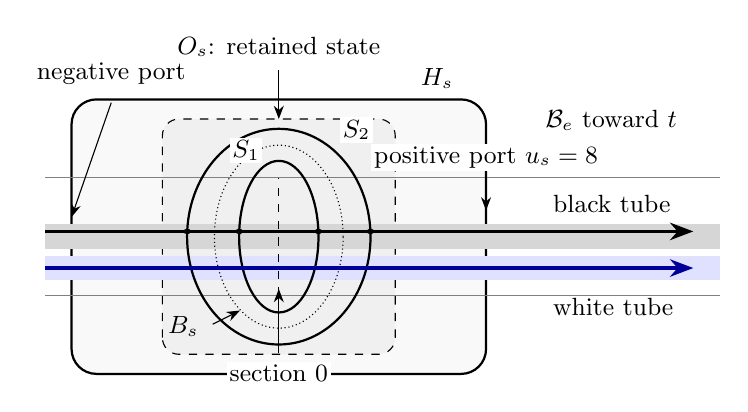
\begin{tikzpicture}[x=1.12cm,y=.83cm,>=Stealth,font=\small]
 \fill[gray!5,rounded corners=9pt] (-2.35,-2.1) rectangle (2.35,2.1);
 \draw[thick,rounded corners=9pt] (-2.35,-2.1) rectangle (2.35,2.1);
 \fill[gray!12,rounded corners=6pt] (-1.32,-1.8) rectangle (1.32,1.8);
 \draw[dashed,rounded corners=6pt] (-1.32,-1.8) rectangle (1.32,1.8);
 \fill[black!16] (-2.65,-.195) rectangle (5.0,.195);
 \fill[blue!12] (-2.65,-.66) rectangle (5.0,-.30);
 \draw[gray] (-2.65,.9)--(5.0,.9);
 \draw[gray] (-2.65,-.9)--(5.0,-.9);
 \draw[thick] (0,0) ellipse [x radius=.45,y radius=1.16];
 \draw[densely dotted] (0,0) ellipse [x radius=.73,y radius=1.40];
 \draw[thick] (0,0) ellipse [x radius=1.04,y radius=1.65];
 \draw[dashed] (0,-.9)--(0,.9);
 \draw[very thick,->] (-2.65,.08)--(4.7,.08);
 \draw[blue!60!black,very thick,->] (-2.65,-.48)--(4.7,-.48);
 \foreach \xx in {-.449,.449,-1.039,1.039}
    \fill (\xx,.08) circle[radius=.042];
 \node[anchor=south west] at (1.50,2.12) {$H_s$};
 \node[anchor=south] at (0,2.60) {$O_s$: retained state};
 \draw[->] (0,2.55)--(0,1.80);
 \node[anchor=south east,fill=white,inner sep=1pt] at (-.18,1.12) {$S_1$};
 \node[anchor=south west,fill=white,inner sep=1pt] at (.69,1.43) {$S_2$};
 \node[anchor=east] at (-.80,-1.37) {$B_s$};
 \draw[->] (-.75,-1.34)--(-.44,-1.13);
 \node[anchor=north,fill=white,inner sep=1pt] at (0,-1.91) {section $0$};
 \draw[->] (0,-1.78)--(0,-.80);
 \node[anchor=south,fill=white,inner sep=1pt] at (2.35,1.0) {positive port $u_s=8$};
 \draw[->] (2.35,.96)--(2.35,.40);
 \node[anchor=south] at (3.77,1.48) {$\mathcal B_e$ toward $t$};
 \node[anchor=west] at (3.0,.50) {black tube};
 \node[anchor=west] at (3.0,-1.08) {white tube};
 \node[anchor=south] at (-1.90,2.18) {negative port};
 \draw[->] (-1.90,2.05)--(-2.35,.30);
\end{tikzpicture}
\caption{A topological schematic of a plug and its outgoing sector.
The two gate circuits have only two black contacts with the displayed
rim passage.  The cutoff lies between the gate annuli.  The state and
the whole sector are retained in comparisons; the success tubes are
strictly inset.  The shapes and radii in this schematic are not to scale.}
\label{fig:plug-sector}
\end{figure}

\begin{lemma}[Conditional bridge]\label{lemma:bridge}
For every fixed connector and admitted endpoint types, there is $c_e>0$
such that, for all sufficiently small $\eps$ and almost every pair of
usable endpoint states,
\begin{equation}\label{plug:success}
 \nu(S_e\mid\sigma_s,\sigma_t)\ge c_e.
\end{equation}
The constants are uniform for rigid copies and for buffered families
with a uniformly bounded number of fixed-shape crossing rectangles.
Moreover, on good continuation geometry, the white part of $S_e$ has a
positive quenched lower bound if the two white side tests each have
conditional probability at least $\beta$ given that geometry and the
inner states.
\end{lemma}

\begin{proof}
Write $A=L_s^+\cap L_t^-$ and $\sigma=(\sigma_s,\sigma_t)$.  The endpoint
exterior restrictions are independent, so $\nu(A\mid\sigma)\ge\beta^2$.
For each color, continue through its open layer by a finite connected
network of buffered crossing corridors.  At each end include a transverse
bar in the nominal slab $5<|u|<6$, crossing the entire corresponding
window with margin; join these bars through the layer.  All continuation
queries lie strictly outside the state disks.  A bar intersects every
successful side path, since that path traverses the slab through the
window.  Retention and buffers allow passage between cell and primal
crossings without changing this separation argument.

Here is the corridor construction in the form that will also be used
for local preparations.  Approximate a compact trace in an open corridor
by finitely many horizontal and vertical polygonal legs on a sufficiently
fine fixed square grid.  Put thin crossing rectangles along the legs,
with both horizontal and vertical crossings in successive overlap
squares, and add the same overlaps at branch points.  Crossing paths
therefore join into the prescribed network.  Slightly lengthening and
shrinking the rectangles leaves room to convert them into retained
primal paths.  Along a charted simple trace the steps may be chosen with
arbitrarily small longitudinal extent, so concatenation in order gives
any prescribed positive bound on longitudinal backtracking.

Let $E$ assert the retained-mesh and quenched rectangle lower bounds in
these finitely many continuation footprints.  Fixed collars keep its
point queries outside $O_s\cup O_t$, independently of the states.
Proposition~\ref{prop:probability-input} and Lemma~\ref{lemma:mesh} give
\[
 \nu(E^c\mid\sigma)\le\delta_\eps\longrightarrow0
\]
uniformly over the usable states.  No good-geometry requirement deep
inside an arbitrary fixed state is needed: its successful side paths
already use retained edges.

Condition now on all point geometry and on $\sigma$.  On sites queried
by black constraints order the bits toward black, and on the disjoint
set queried by white constraints order them toward white.  Both $A$ and
the continuation success $K$ are increasing in this one product order;
constraints of the same color may overlap.  The two sets of colors have
positive separation by the layer and chart-tolerance margins.  On $E$,
conditional positive association and the crossing input give
\[
 \nu(A\cap K\mid\eta,\sigma)
 \ge \nu(A\mid\eta,\sigma)\nu(K\mid\eta,\sigma)
 \ge q_e\nu(A\mid\eta,\sigma),
\]
where $q_e>0$ is fixed.  Since $A\cap K\cap E\subset S_e$, integration
before subtraction yields
\[
 \nu(S_e\mid\sigma)
 \ge q_e\nu(A\cap E\mid\sigma)
 \ge q_e(\beta^2-\delta_\eps).
\]
This proves \eqref{plug:success}.  It does not infer any quenched black
side propensity from an annealed one.  If the two white side propensities
are themselves bounded below after fixing geometry, the white-only
version of the same product argument gives $q_e^W\beta^2$ without this
annealed integration.  For fixed normalized templates, finitely many
buffered rectangle chains give common positive constants by scaling;
rigid motions preserve the laws.
\end{proof}

\subsection{Cycle experiments and exact path agreement}

\begin{definition}[Cycle experiment]\label{def:cycle-experiment}
For a simple system, sample the states independently with their laws
$\mu_s$.  Given the states, sample the exterior regions of the connectors
independently, each conditioned on its success $S_e$, and sample the
remaining plane data ordinarily.  The exterior region of $e$ may be the
whole sector $\mathcal B_e$ with the closed endpoint state disks removed.
\end{definition}

All queries of $S_e$ are then in its region or its endpoint states, for
small $\eps$.  The cycle law has density
\begin{equation}\label{plug:cycle-density}
 \prod_s\frac{\ind_{G_s}}{\nu(G_s)}
 \prod_{e:s\to t}
 \frac{\ind_{S_e}}{\nu(S_e\mid\sigma_s,\sigma_t)}
\end{equation}
relative to $\nu$ on these data; unused data remain free.  Thus it is
boundedly dominated by $\nu$ for a fixed system.  In particular, the
marginal of two endpoint states and one sector is exactly their ordinary
law restricted by the three factors for $G_s,G_t,S_e$.  Deterministic
Borel restrictions suffice throughout: a Jordan boundary need not be
smooth or have zero area.

\begin{lemma}[A confined rim and its gate passages]\label{lemma:cycle-rim}
On a cycle experiment, outside an event of probability tending to zero,
there is a rim $P$ of the path color, oriented in the positive longitude,
contained in the layer $-2.35<v<.8$.  At every selected gate circuit it
has exactly two contacts, crossing from the negative side into the
interior and then out through the positive side.  Its outside path from
the first-gate exit at $s$ to the first-gate entry at $t$ lies in
$\mathcal B_e$.  The inner gate paths occur in the prescribed cyclic
order.
\end{lemma}

\begin{proof}
The root components join negative to positive side vertices within their
central windows.  Concatenate these paths with the successful sector
paths.  For both colors one obtains a monochromatic closed walk of
longitudinal index one, respectively in the disjoint layers
$-.75<v<.75$ and $-2.3<v<-.9$.  This index follows by lifting the
longitude: root passages cross the central slabs, and sector passages go
from one positive slab to the next negative one without passing the end
section cuts.  Arbitrary local backtracking is harmless.  Fine mesh
keeps the edge segments in the stated layers.  Each walk contains an
essential simple circuit.  Lemma~\ref{lemma:sandwich} supplies a black
rim between them.  The farther subbands on either side lie in the two
exterior sides of this sandwich, so the chosen rim is confined to
$-2.35<v<.8$.

This rim visits both the inside and outside of either gate: it crosses
section $0$ deep inside and also reaches the other plugs.  A black rim
can meet a gate with at most two black sites only at those sites.  By
simplicity it must meet exactly two, once each, and cross at both.  A
tangency would not change side, leaving too few contacts.  Following a
gate edge between the two contacts is also impossible: the complementary
rim arc would then have to visit both sides without another contact.
Thus the incoming and outgoing edges are strictly in opposite gate fans.

All visits to the central section belong to the single inner gate arc.
That arc lies in the end chart, since the gate and its bounded inside lie
in $O$ and all other bands avoid its obstacle.  The full central slab is
inside the first gate, and compact positive and negative chart portions
meeting the gates are separated.  The total positive longitudinal index
one therefore forces negative entry and positive exit.  This uses
ordered passage, or equivalently lifted longitude, without requiring a
transversal intersection with section $0$.  Outside its inner first-gate
arc the rim cannot cross that section.  Consequently the outside arc
from $s$ to the next $t$ stays in their intervening sector.  Since each
inner arc contains all visits to its own cut and these chart slabs are
disjoint, the inner arcs have the asserted cyclic order.
\end{proof}

The following formulation isolates the precise deterministic comparison
that will also apply to rims in different configurations.

\begin{lemma}[Two-graph gate consistency]\label{lemma:gate-consistency}
Let $P,P'$ be oriented simple monochromatic rims in their respective
embedded triangulations.  Suppose their directed subpaths $\gamma,
\gamma'$ have common distinct initial and terminal vertices $v,w$ and
satisfy these conditions:
\begin{enumerate}[label=\textup{(\roman*)}]
\item each \emph{complete compared subpath} is present and monochromatic
in the other graph, with the same embedding;
\item at $v$ there is a shared gate circuit, both incoming rim rays lie
strictly in one gate fan, and both outgoing rays lie strictly in the
opposite fan;
\item the rim orientations and direction of crossing that gate agree.
\end{enumerate}
Then $\gamma=\gamma'$ as directed edge paths.  Each rim needs its
no-right-bypass property only in its own graph.
\end{lemma}

\begin{proof}
Order rays in the outgoing fan counterclockwise between its two boundary
rays.  For any incoming ray in the opposite open fan, the
counterclockwise sector from that ray to an outgoing ray contains the
same initial portion of the outgoing fan.  Hence, if the two outgoing
rays differ, one enters the other's open right sector, independently of
the differing incoming rays.  Suppose, for instance, that $\gamma'$
leaves to the right of $P$.

Follow $\gamma'$ to its first subsequent contact with the \emph{whole}
rim $P$, not merely with $\gamma$.  Such a contact exists no later than
$w$.  It is not $v$, because $\gamma'$ is simple.  As $\gamma'$ is a path
in $P$'s graph, planarity makes the first contact a vertex contact; a
shared edge is first reached at its endpoint.  Before this contact the
path is connected and disjoint from $P$, so it stays in the open right
component into which it departed.  It is therefore a monochromatic
right bypass between distinct vertices of $P$, contradicting
Lemma~\ref{lemma:no-bypass}.  An earlier return on the complementary
portion of $P$ gives exactly the same contradiction.  The other case
uses $P'$ in its own graph.

Thus the first edges agree.  At any later first divergence the incoming
edge is common, and cyclic order from that incoming ray again puts one
outgoing edge into the other's open right sector.  The same whole-rim
first-return argument rules this out.  The paths agree to $w$.
\end{proof}

\begin{lemma}[Deterministic collars for the compared paths]
\label{lemma:fixed-collar}
For a fixed cycle pattern, every possible confined experiment rim has
its inner second-gate path in a fixed compact subset of its state disk.
Every possible first-exit-to-next-first-entry path lies in a fixed
compact subset of
\[
 D_e=O_s\cup O_t\cup\mathcal B_e.
\]
Consequently, if two configurations retain these data, their complete
incident triangulations along the compared paths agree on the mesh-good
event, for all sufficiently small $\eps$.
\end{lemma}

\begin{proof}
The second gate is in its prescribed outer ball, compactly inside $O$;
its bounded inside is in the same ball.  This gives one deterministic
envelope, also containing the gate neighborhoods.  For an outside path
use the closed inset footprint $-2.35\le v\le.8$ in the whole sector.
It has positive lateral margins.  The chart--connector seams are
interior product-band seams.  At the two longitudinal ends the full
section and a central slab are compactly inside the endpoint states,
which shield the cuts.  Hence this footprint is compactly contained in
$\operatorname{int}D_e$.  Its collar is fixed before selecting a rim;
there is no requirement that the rim follow a particular witness of
$S_e$.

If a triangle is incident to a vertex in such an envelope and its
circumradius is at most $\rho_{\eps,h}$, its whole circumdisk is within
$2\rho_{\eps,h}$ of that envelope.  For small $\eps$ the disk lies in
the retained region, so its vertices and empty-circumdisk condition are
unchanged.  Mesh control in \emph{both} configurations excludes additional
large incident triangles on either side.  Thus all incident triangles,
not only the edges of a preselected path, agree.  The required mesh
probabilities follow from ordinary control and the fixed density bounds
for the experiments.
\end{proof}

For coupled cycle experiments sharing a state, choose the same
deterministic gate circuits from that state.  By
Lemma~\ref{lemma:cycle-rim}, both rims visit the inside and outside of
each chosen gate and can meet it only at its at most two path-color
vertices.  They therefore use the same two distinct vertices; negative
entry and positive exit give the same ordering of these contacts.  Thus
the inner second-gate paths have common ordered endpoints, and the
outside paths from the first-gate exit at $s$ to the first-gate entry at
$t$ do also when both endpoint states are shared; these endpoints are
distinct because the state disks are disjoint.  At the start of an
inner path, both incoming rays are in the exterior gate fan and both
outgoing rays in the interior fan; at the start of an outside path these
roles are reversed.  All these inclusions are strict.  Sharing the state
preserves the colored collar of each complete inner second-gate path;
sharing both endpoint states and the whole sector does the same for
each complete outside path.  On the mesh-good event,
Lemma~\ref{lemma:fixed-collar} therefore puts each compared path in the
other graph with the same colors and preserves every incident triangle.
Lemma~\ref{lemma:gate-consistency} now identifies the directed paths.
Their right incident triangles and local tagged sides consequently
agree as well.  The allowed chart changes preserve the sign and collar
margins used in this argument.

\subsection{Removing the exterior randomness}

On a cycle experiment choose any measurable confined rim as above.
For $X=Q,V$ define
\begin{equation}\label{plug:masses}
 \widehat m_s=X_P(\ind_{B_s}),\qquad
 \widehat j_e=X_P\bigl(\ind_{\mathcal B_e\setminus(B_s\cup B_t)}\bigr),
 \qquad e:s\to t.
\end{equation}
These are barycenter masks.  Fix disjoint Borel conventions at sector
boundaries; the rim is buffered away from lateral boundaries and the
section cuts are inside cutoff balls.  One may set the masses to zero
on the exceptional geometry event.  The deterministic-mask energy
bound \eqref{fields:energy}, ordinary triangle moments and bounded cycle
density give finite $L^2$ bounds for each fixed pattern.  For bounded
normalized short templates with common density bounds these norms are
at most $C h$.

Every cutoff tag comes from the inner path through the \emph{second}
gates, because the cutoff is buffered inside that gate.  The sector
mass is precisely the contribution outside both cutoff balls along the
path from the \emph{first} exit at $s$ to the first entry at $t$:
the inner first-gate paths and cuts lie safely inside the balls.  Thus,
on the mesh-good event,
\[
 \sum_{e:s\to t}(\widehat m_s+\widehat j_e)=X_P(1).
\]

\newpage
\begin{proposition}[The state cochain]\label{prop:state-cochain}
For every fixed connector, including its actual end charts, there are
functions $i_e^\eps(\sigma_s,\sigma_t)$ such that
\begin{equation}\label{plug:cycle}
 \begin{aligned}
 \widehat m_s+\widehat j_e-i_e^\eps&=o_{L^1}(1)
       &&\text{in every cycle experiment containing }e,\\
 \sum_e i_e^\eps&=o_{L^1}(1)
       &&\text{on the independent state product of every simple system}.
 \end{aligned}
\end{equation}
The same functions work in all completions.  For a fixed collection of
normalized short templates admitting uniform short completions,
\[
 \|i_e^\eps\|_{L^2(\mu_s\otimes\mu_t)}\le C h
\]
for all sufficiently small $\eps$, after increasing a common constant.
\end{proposition}

\begin{proof}
For each type, fix a short unperturbed reference completion, for example
using a sufficiently separated copy.  Define $m_s^\eps(\sigma_s)$ as
the conditional mean of its cutoff mass given $\sigma_s$.  Couple any
other experiment to this completion sharing only that state and sampling
the remaining data conditionally independently.  Inner second-gate
consistency identifies the cutoff mass on their common mesh-good event.
Their $L^2$ bounds show that their difference is $o_{L^1}(1)$; indeed
$\EE[|Y|\ind_E]\le\|Y\|_2\PP(E)^{1/2}$ on a bad event $E$.
Using two copies also in the reference completion and conditional Jensen
shows that its mass is $o_{L^1}(1)$ from its own conditional mean.
Consequently $\widehat m_s=m_s^\eps+o_{L^1}(1)$ in every completion.

Next fix one two-plug completion of $e$ and condition its sector mass on
$\sigma_s,\sigma_t$ and the exterior sector datum $\xi_e$.  Call the
result $j_e^\eps(\sigma_s,\sigma_t,\xi_e)$.  These retained data have
the same marginal in every completion, by \eqref{plug:cycle-density}.
Coupling and outside first-gate consistency, again with a second copy
for the defining completion, give
$\widehat j_e=j_e^\eps+o_{L^1}(1)$ in every experiment containing $e$.

In a fixed cycle, conditional on its complete state vector, the data
$\xi_e$ are independent, each with the conditioned law determined by its
two endpoint states.  The closed estimate \eqref{fields:closed} and the
cycle density show that
\[
 \sum_e(m_s^\eps+j_e^\eps)=o_{L^1}(1).
\]
For $Q$ the selected rim is contained in a fixed box and has a fixed
positive minimum diameter, since it visits distinct plugs; for $V$ its
complete tangent sum is zero.  Now resample one $\xi_e$ independently
given the states, leaving all other sectors fixed.  Subtracting the two
small cycle sums gives $j_e^\eps-(j_e^\eps)'=o_{L^1}(1)$.  Conditional
Jensen therefore gives
\[
 j_e^\eps-
 \EE[j_e^\eps\mid\sigma_s,\sigma_t]=o_{L^1}(1).
\]
The conditional law used in this last expectation depends only on those
two states.  Set
\[
 i_e^\eps=m_s^\eps+
         \EE[j_e^\eps\mid\sigma_s,\sigma_t].
\]
This proves both statements in \eqref{plug:cycle}.  The defining short
completions and Jensen give the stated $L^2$ bounds.  All replacements
use only bounded second moments and high-probability path equality;
uniform integrability of their squares is unnecessary.  The choices
are measurable because the locally finite graphs have countably many
finite paths and walls, and different choices agree through the same
path comparison.
\end{proof}

\subsection{Common closures, collars and changes of charts}

\begin{lemma}[Comparison by a common closure]\label{lemma:common-closure}
Suppose two directed paths of connectors from $s$ to $t$ admit a common
complementary connector $c:t\to s$, making each a simple system.  Their
sums of cochain values differ by $o_{L^1}(1)$ on the product of all states,
with shared states identified.  Either path may be a single connector.
For fixed end disks and charts, a connector value therefore depends,
up to $o_{L^1}(1)$, only on the endpoint-fixed deformation class of its
exterior simple centerline described below.
\end{lemma}

\begin{proof}
Apply \eqref{plug:cycle} to the two cycles and subtract the common
$i_c^\eps$.  Adding independent unused states does not change an $L^1$
error.  A complementary connector always exists: two disjoint closed
Jordan disks joined by the attached rectangular band form a Jordan disk,
with the unused ports on its boundary.  In its exterior, the
Jordan--Schoenflies theorem gives another handle band joining those
ports.  The transverse parametrizations match because departure and
arrival sections have opposite induced boundary orders.  The remaining
deformation assertion follows from the collar construction and finite
chaining below.
\end{proof}

\begin{lemma}[A band with prescribed full attachments]\label{lemma:band-collar}
Let a simple exterior arc join the middle points of two prescribed port
sections.  Suppose it continues for a short distance along the given
product collars at its ends and otherwise avoids the closed end disks.
Then a rectangular band about it, with those full parameterized
attachments, fits in any neighborhood of the arc and attachments within
the exterior.  It can in addition avoid any fixed disjoint compact
routes or unused obstacles.
\end{lemma}

\begin{proof}
Extend a short piece of each given end collar and taper its transverse
width to be very small at the far tip.  The full port is usable initially:
the compact middle arc is separated from it, while the given product
collar handles its immediate neighborhood.  Straighten a slightly
extended middle arc by an orientation-preserving plane arc chart, with
its left side above a horizontal segment.

From the upper and lower corners of each narrow collar tip, follow
constant small signed transverse coordinates in that end collar for a
short additional distance.  In the straightened coordinates these side
paths lie on the corresponding sides of the midline and progress along
it with arbitrarily small error.  Stop at their first hits of prescribed
vertical lines, chosen in order at the two ends.  Join the upper stopped
paths, and separately the lower ones, by height graphs strictly on their
side of the middle segment and as close to it as desired.  The compact
middle interval is separated from the initial collar pieces and disks,
so these joins fit in the specified neighborhood and avoid all the
specified compact sets.  First-hit stopping keeps the side paths simple.

Each joined side, the appropriate half-tip segments and the centerline
bound a Jordan rectangle.  The two rectangles lie on opposite sides in
the straightened coordinates and may be taken thin there.  The initial
disk-with-collar interiors abut their tips on the other side, so they
cannot cross either boundary curve.  Fill the rectangles by
Jordan--Schoenflies, prescribing the centerline and boundary
parametrizations, and glue them to the end collars.  This gives the
required band with the full original port attachments.
\end{proof}

For completeness, the deformation in
Lemma~\ref{lemma:common-closure} is implemented as follows.  Normalize
the disjoint Jordan disks to round holes by an ambient homeomorphism.
Inside an existing exterior band replace its centerline by a smooth
proper arc, radial near its endpoints, retaining the same complementary
connector.  Indeed an attaching section has a relative exterior
neighborhood; polygonal approximation in this open set, loop erasure
and smoothing give a simple arc with the prescribed short radial germs.
The full port attachments are recovered by
Lemma~\ref{lemma:band-collar}.

Consider now an endpoint-fixed deformation through smooth proper arcs,
transverse at the hole boundaries.  Product end collars are available
throughout, adjusting their angular coordinate with the radial level
near each endpoint.  At a parameter value choose a narrow connector and
a complementary band disjoint from it.  By compact separation that
complement also avoids all nearby centerlines; the collar lemma supplies
connectors for them with the same full attachments.  At overlapping
parameter neighborhoods, narrow a connector to avoid both choices of
complement.  A finite subcover of the parameter interval and the
common-closure comparison give the $o_{L^1}(1)$ equality along the whole
deformation.  Constants may depend on this finite chain, which is fixed
before $\eps\downarrow0$.

\begin{lemma}[Stability on buffered local templates]\label{lemma:chart-stability}
Fix a buffered two-plug system $e_0,c_0$.  Suppose its parts in the preset
neighborhoods where charts may move are fixed local stubs, and no other
part of the system returns to these neighborhoods.  For sufficiently
small supported changes $g$ of the two end charts and obstacles, let
$e_g,c_g$ be the corresponding images.  Then
\[
 i_{e_g}^\eps=i_{e_0}^\eps+o_{L^1}(1)
       \quad\text{on }\mu_s\otimes\mu_t.
\]
The required tolerance depends only on the compact local stub and layer
margins in the moved regions.
\end{lemma}

\begin{proof}
Consider the mixed experiment with successes $S_{e_g}$ and $S_{c_0}$,
with the nominal states and roots.  Their exterior queries are still
separated, and Lemma~\ref{lemma:bridge} applies.  All allowed tubes lie
in slightly widened, separated layers of the nominal annular band,
with the same longitudinal order.  This follows by the local tolerance
where anything moved; elsewhere the system is unchanged.  Thus the mixed
experiment has the same confined-rim and gate conclusions, and we may
use deterministic nominal masks for its masses.

Compare its $e$ contribution with the pure $e_g,c_g$ experiment by
sharing the states and the exterior part of the \emph{nominal} $e_0$
sector.  Every possible pulled-forward inset $e_g$ path outside the
states, together with all queries of $S_{e_g}$, is buffered in that
shared region.  The queries of both $S_{c_g}$ and $S_{c_0}$ avoid it.
Consequently the shared marginal in both experiments is the ordinary
one conditioned on $S_{e_g}$ at the two sampled states: the other
success factor integrates to one given the states and affects only
other exterior data.  This also follows directly from the product
density \eqref{plug:cycle-density}, irrespective of how unused points
are assigned to the sampling regions.

The common collar and the two gate comparisons identify the first-gate
path outside the cutoff balls and the starting cutoff contribution.
Thus the extracted $e$ value in the mixed experiment is $i_{e_g}^\eps$
up to $o_{L^1}(1)$.  The same argument identifies its other contribution
with $i_{c_0}^\eps$.  Closing the mixed rim therefore gives
$i_{e_g}^\eps+i_{c_0}^\eps=o_{L^1}(1)$, whereas the nominal system gives
$i_{e_0}^\eps+i_{c_0}^\eps=o_{L^1}(1)$.  Subtraction proves the claim.
\end{proof}

The restriction to buffered local templates is deliberate.  An
arbitrarily thin fitted connector with changed charts is first deformed
with those changed charts held fixed.  Only its standard buffered
representative is then compared to the nominal charts by
Lemma~\ref{lemma:chart-stability}.  A narrow fitted band's conditioning
constant is never used as the uniform constant of a short-template
moment estimate.

\section{The affine part and endpoint potentials}\label{sec:affine}

The state cochain now separates into a spatially affine term and two
local endpoint terms. Short comparison experiments control the endpoint
terms uniformly; the geometry of a long connector enters only a
controlled deterministic remainder.

Fix a finite normalized menu.  Actual placements may be its translates
on the $h$-grid; auxiliary translated and rotated copies are also allowed.
At fixed $h$, pass to a further subsequence on which the admissions
stabilize.  If any type is admitted, choose one reference type and its
color flip.  When the admitted menu is empty all comparisons at qualified
endpoints are vacuous; we may set $a_h^V=1$ and choose any bounded $a_h^Q$.

\subsection{Fixed stubs and straight means}

For each type fix two disjoint \emph{stubs} outside its obstacle, taking
the departure port to an eastward horizontal strip and the arrival port
to a westward horizontal strip.  Their exit sections lie at the midpoints
of opposite sides of a sufficiently large square, with transverse
coordinate $v$ increasing upward.  To construct them, use a Jordan
annulus between the obstacle and the square, match the two attachment
intervals in cyclic order, and draw disjoint product continuations.
The transverse order is along the positive boundary direction at the
east exit and against it at the west exit, precisely as required by the
departure and arrival ports.  Continue the strips straight outward.

Fix the local portions of the stubs and their positive margins in all
regions where chart changes may be supported before placing other
plugs.  A later enlargement of the exit square uses only straight
continuation.  Rotate a type together with its stubs whenever needed.
These choices meet the local-template hypotheses of
Lemma~\ref{lemma:chart-stability}.

\begin{proposition}[Affine straight means]\label{prop:affine}
For $X=Q,V$ there is a scalar $a_h^X$, uniformly bounded in $h$, such
that every fixed straight transport in the countable family used below
has mean
\begin{equation}\label{affine:means}
 \EE_\mu i_e^\eps=a_h^X(z_t-z_s)+o(1).
\end{equation}
The same scalar applies to translations, common rotations and color
flips of the reference type.  All choices can be made simultaneously
for the two fields and countably many $h$.
\end{proposition}

\begin{proof}
Join identical unrotated reference copies on a horizontal line, using
their fixed stubs and a straight gap.  Their center separation is
$\ell h$, where $\ell>D$ for a fixed sufficiently large $D$.  Write
$A_\eps^X(\ell)=\EE_\mu i_e^\eps$.  A remote complementary connector
through the unused stubs closes both this transport of length
$(\ell+r)h$ and the two transports obtained by inserting a middle
reference copy.  Lemma~\ref{lemma:common-closure} gives
\[
 A_\eps^X(\ell+r)=A_\eps^X(\ell)+A_\eps^X(r)+o(1),
       \qquad \ell,r>D.
\]
Translation and rotation of the entire experiment, including the root
ordering, preserve its law and rotate both fields as vectors.  If a
conditional-average or gate tie-breaking convention was chosen
separately at the translated placement, its transported version is an
alternative defining completion.  Gate consistency with common gates
in the shared states and Proposition~\ref{prop:state-cochain} compare
the two choices to $o_{L^1}(1)$.  Thus covariance to this accuracy is
sufficient.  Color exchange preserves the law as well.

The ratios $A_\eps^X(\ell)/h$ are bounded uniformly for
$D+1\le\ell\le D+4$, in the limit superior: these transports have
bounded normalized size and uniformly buffered short completions.
For each fixed larger length there is likewise a finite bound, not
necessarily uniform in that length.

Only countably many lengths are required: the standard routes below
are fixed by grid terminal pairs, finitely many types and integer twists.
Include the positive integers and take the rational span of these
lengths, a countable additive subgroup $\mathcal L\subset\R$.  Extract
limits of $A_\eps^X(\ell)/h$ for all $\ell\in\mathcal L$ with $\ell>D$.
Their function $A$ is additive whenever both arguments exceed $D$.
Extend it to $x\in\mathcal L$ by
\[
 \widetilde A(x)=A(u+x)-A(u),\qquad u,u+x>D.
\]
The value is independent of a sufficiently large $u$: comparing two
choices $u,v$ uses
$A(u+x)+A(v)=A(u+v+x)=A(v+x)+A(u)$.
Choosing all offsets large similarly proves additivity on $\mathcal L$.
For small $x$, take a fixed rational $u$ in the interior of
$[D+1,D+4]$; the interval bound gives a common bound on
$\widetilde A(x)$.  Additivity then gives continuity at zero: if
$|x|<\delta/N$, a bound for $\widetilde A(Nx)$ gives the same bound
divided by $N$ for $\widetilde A(x)$.  Since $\mathcal L$ contains the
rationals, continuity implies $\widetilde A(x)=a_h^X x$.  The interval
bound also bounds $|a_h^X|$ independently of $h$.  Covariance yields
\eqref{affine:means} in every direction.  Countable diagonal extraction
makes these choices simultaneously as asserted.
\end{proof}

\subsection{Normalization of the tangent field}

\begin{lemma}\label{lemma:tangent-normalization}
The scalar of the tangent field is
\begin{equation}\label{affine:tangent}
 a_h^V=1.
\end{equation}
\end{lemma}

\begin{proof}
We give the mask argument also for curvilinear end charts.  In an
unperturbed straight experiment choose a deterministic polygonal Jordan
quadrilateral $R_e$ approximating the sector from section $0$ to section
$0$ with transverse interval $[-2.7,1.5]$.  Its boundary is close in the
ordered parametrization.  The transverse end cuts remain in the first
gate balls, and its top and bottom sides lie beyond the possible rim
layer $[-2.35,.8]$ on its left and right, respectively.  Permit a small
longitudinal enlargement only inside the cutoff balls.  By compact
margins, outside slightly smaller cutoff balls the mask contains exactly
the relevant sector side of every confined rim, with room, and excludes
the complementary side.

Here the required polygonal approximation follows directly from Jordan
simplicity.  Trace a polygonal closed walk uniformly close to the
boundary in order, split any crossings in general position and retain
a simple subcycle with positive winding about a fixed inner point.
Dropped parameter gaps have endpoints tending together, and therefore
are short by injectivity of the limiting Jordan parametrization.  They
cannot be almost a whole turn: the retained cycle would then be local
and have zero winding about the inner point.  This preserves the ordered
approximation and the four chosen sides.  Fix one such quadrilateral in
a sufficiently long template.  For larger $\ell$, stretch only its
straight middle region horizontally, keeping both end regions rigid.
The margins persist for each fixed $\ell$, and the total length of the
two end cuts is $O(h)$ uniformly in $\ell$.

On good geometry, polygonal intersection with the left side of $P$
gives
\[
 \int_{P\cap R_e}\dd z=\ell h+O(h).
\]
Indeed this integral is minus the integral over the portion of
$\partial R_e$ on that left side.  The entire top side contributes with
reversed orientation, the bottom side does not contribute, and the end
cuts cost $O(h)$.  Their endpoint locations differ from the plug centers
by $O(h)$.  A fixed cut has probability zero of an accidental exact
overlap with a random primal edge or vertex degeneracy.

We next compare this geometric integral with the barycenter mask
$V_P(\ind_{R_e})$.  On fine mesh a discrepancy can involve only rim
edges whose tagged triangles meet a cut segment.  Put $s=\eps^\alpha$
with $\alpha<1$ sufficiently close to one and cover these finitely many
segments by $O_e(s^{-1})$ boxes of side $s$.  In any one enlarged box the
$L^2$ norm of the total candidate edge length is $O(s^2/\eps)$, by the
scaled local triangle moments.  The presence of a candidate rim edge
implies a monochromatic arm from scale $s$ to a fixed positive distance
for this pattern, since the rim also visits a different plug.  Its
ordinary probability is $O_e(s^c)$, apart from a negligible mesh event.
Cauchy--Schwarz and summation thus bound the expected discrepancy by
\[
 C_e s^{-1}\frac{s^2}{\eps}s^{c/2}
       =C_e\eps^{\alpha(1+c/2)-1}\longrightarrow0
\]
when $\alpha>1/(1+c/2)$.  Bad mesh events are discarded using the same
local moments.  The bounded density of this fixed experiment transfers
the assertion to its law.  Alternatively, convergence in probability
and the Bessel $L^2$ bound suffice for the corresponding mean limit.

Outside the two cutoff balls, $R_e$ gives exactly $\widehat j_e$.
Its difference from $\widehat m_s+\widehat j_e$ consists of deterministic
masks inside the endpoint cutoff balls.  Couple at either endpoint state
to a fixed short completion.  The inner second-gate paths and their
triangles agree, so these correction means are $O(h)+o(1)$ by the short
second-moment estimate.  Their constant is independent of $\ell$:
the end masks were fixed before the middle strip was stretched.  By
Proposition~\ref{prop:state-cochain} and \eqref{affine:means},
\[
 |a_h^V\ell-\ell|\le C
\]
for arbitrarily large positive integers $\ell$.  This proves
\eqref{affine:tangent}.
\end{proof}

\subsection{The two endpoint twists}

We next compare an arbitrary fixed connector to a controlled standard
representative.  Its class is understood with the end disks, port
points and charts fixed.

\begin{lemma}[Classification by endpoint twists]\label{lemma:two-twists}
After normalizing the two disjoint Jordan obstacles to round holes,
every exterior simple centerline can be replaced, by common-closure
comparisons, by a smooth proper arc radial at its ends.  Such arcs with
fixed endpoints are classified, for the comparisons needed here, by two
integer endpoint twists.  Relative to a standard route with bounded
endpoint turns, their total size $k$ is bounded by a constant plus a
constant times the sum of the absolute net argument changes about the
two centers along the exterior arc.
\end{lemma}

\begin{proof}
The smoothing and full-port collars were established after
Lemma~\ref{lemma:band-collar}.  Identify each hole boundary with the
circle of directions at its center.  Fix a radial identification of the
plane with the two punctures blown up and the exterior of the circular
holes: in disjoint neighborhoods of the centers, send radius zero to the
hole radius by an increasing radial coordinate, agreeing with the
identity outside those neighborhoods.  Apply its inverse to each
radial-ended proper arc and fill in the punctures.  The result is a
smooth embedded compact interval, radial near its ends, and the fixed
identification recovers exactly the original proper arc after blowing
up.  Any two such smooth intervals, with ordered endpoints
matched, are carried one to the other by an orientation-preserving plane
diffeomorphism. To obtain this smooth extension, first map smooth
strip-and-cap neighborhoods of the two intervals by an
orientation-preserving diffeomorphism, preserving their ordered axes.
Choose smooth disk boundaries inside these neighborhoods. The prescribed
Jordan--Schoenflies theorem extends this map across their complementary
surfaces, retaining its smooth values on collars of those boundaries.
Hatcher's smoothing theorem for surface homeomorphisms, in its form
relative to a boundary neighborhood
\cite[Theorem~B and the following refinement, p.~2]{Hatcher2025},
replaces the exterior homeomorphism by a diffeomorphism without changing
these collars. Gluing with the retained neighborhood map gives the
required plane diffeomorphism and preserves the two intervals and their
endpoints exactly.

An orientation-preserving plane diffeomorphism has a locally smooth
deformation to the identity.  After subtracting its value at a base
point, the maps $x\mapsto F(tx)/t$ tend on compact sets to its positive
differential as $t\downarrow0$; restore the translation and join the
positive linear map to the identity.  During the resulting deformation
of the interval, postcompose by the unique direct similarity restoring
the two current ordered endpoint positions to the two fixed punctures.
This correction is the identity at both ends of the deformation.
Thus the punctures stay fixed throughout.

Blowing up their directions gives a deformation of proper arcs whose
ends move on the two hole circles.  Lift both moving endpoint angles to
real-valued continuous functions.  Compensate each angle in a disjoint
boundary collar, tapering the compensating rotation to zero away from
that boundary.  The deformation now fixes the port points.  At its end
the two compensations are integral full twists, since the original and
final port points agree.  These are the only possible differences
between the fixed-end deformation classes.  The compensated arcs are
transverse to the hole circles.  Compactness of the parameter interval
provides uniformly small product collars in which all these transverse
germs can be straightened to radial germs, continuously in the
parameter.  Take the straightening correction to be the identity at
both terminal times, where the germs are already radial.  The resulting
deformation therefore has the full fixed-end collar form required for
the common-closure comparisons.

They are detected separately by net arguments.  For the starting
puncture, lift the argument along the deforming arc.  The difference of
its final and initial net argument changes is minus the net turn of the
starting direction loop: the direction at the other puncture has zero
net argument change about the starting puncture.  For the arriving
puncture the analogous identity has the opposite sign.  Hence equal
net argument changes at both centers make both compensations trivial
at the end, giving an endpoint-fixed deformation of the kind used in
Lemma~\ref{lemma:common-closure}.  Conversely integer full turns at the
ends realize the corresponding changes; the explicit disjoint
representatives are constructed below.

Choose the signs of the two integers so they record the additional
argument turns in the orientation from $s$ to $t$.  Their absolute sum
is bounded by the displayed net changes divided by $2\pi$, plus the
bounded turns of the reference route.  Normalizing the Jordan disks
does not change winding differences between two arcs with the same
ends: these differences are integer winding numbers of their joined
closed curves about the respective centers.  For allowed perturbed
charts, pull the route back first to the nominal disks.  The arc stays
outside the fixed central balls, and the small supported change has
only a bounded effect on the endpoint argument choices.  This gives
the same bound for $k$ up to a fixed additive constant.
\end{proof}

\subsection{Quantitative standard representatives}

For each terminal type choose a fixed short start insertion: go east
along its departure stub to a horizontally aligned reference copy at a
fixed large distance.  Choose a fixed short end insertion from a
reference copy west of the arriving terminal into its arrival stub.
Their distances are large enough for the full local structures and the
supports of chart changes; all these lengths are nevertheless fixed in
normalized units.  They have uniformly bounded short standalone
completions and hence the $C h$ cochain bounds.  The first and last
insertions will remain fixed when the long route changes.

\begin{lemma}[Standard spirals and short corner templates]
\label{lemma:standard-spirals}
Fix nominal terminal placements, their types and two twist integers
$n_s,n_t$, and put $k=|n_s|+|n_t|$.  There is a constant $C$ such that,
if
\[
 |z_t-z_s|>Ch(1+k),
\]
the class has a buffered representative beginning and ending with the
fixed insertions above.  Between them it consists of straight transports
and at most $C(1+k)$ short pieces.  The short pieces belong, up to rigid
motion, to uniformly buffered compact families of bounded normalized
size, and satisfy
\[
 \|i_j^\eps\|_{L^2}\le C_{\rm short}h
\]
for small $\eps$, with a constant independent of the terminal separation,
the twists and the particular long connector.

A common complementary connector closes both the inserted path and its
unsplit representative.  All auxiliary placements and straight lengths
can be fixed from the nominal terminal data and integers before making
allowed chart changes.  In the applications they form a countable list.
\end{lemma}


The three features of this representative have different roles in the
cochain comparison. Its fixed first and last insertions determine the
endpoint state functions. Its straight pieces, however long, have the
exact limiting means in Proposition~\ref{prop:affine}. Only the
$O(1+k)$ short pieces contribute an $O(h(1+k))$ deterministic error.
Figure~\ref{fig:standard-representative} shows how the used route and a
common complement can turn around the terminals without meeting.
We first derive the endpoint formula from these properties; the full
geometric construction follows after that proof.

\begin{figure}[tb]
\centering
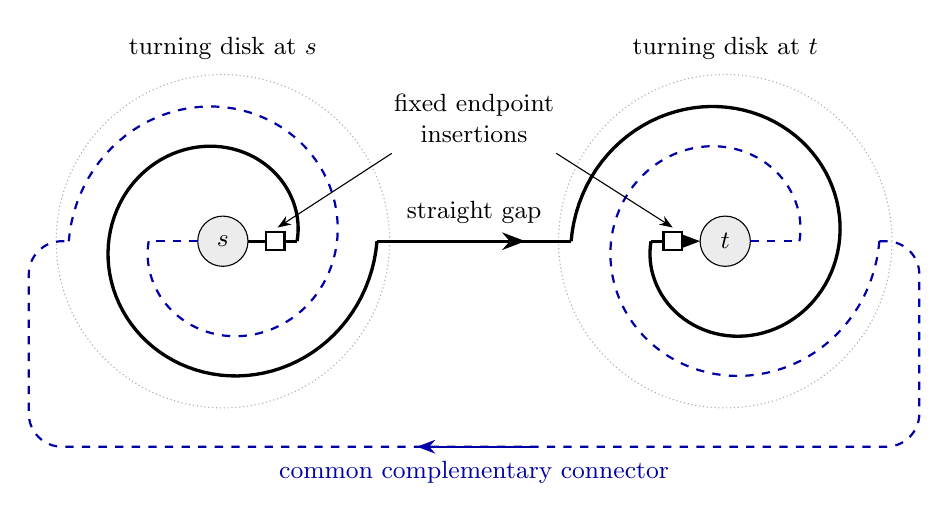
\begin{tikzpicture}[x=1.45cm,y=1.45cm,>=Stealth,font=\small]
 \draw[gray!65,densely dotted] (0,0) circle[radius=1.46];
 \draw[gray!65,densely dotted] (4.4,0) circle[radius=1.46];
 \filldraw[fill=gray!15,draw=black] (0,0) circle[radius=.22];
 \filldraw[fill=gray!15,draw=black] (4.4,0) circle[radius=.22];
 \node at (0,0) {$s$};
 \node at (4.4,0) {$t$};
 \draw[very thick] (.22,0)--(.65,0);
 \draw[very thick,domain=0:360,samples=100,variable=\u]
       plot ({(.65+.70*\u/360)*cos(\u)},
             {(.65+.70*\u/360)*sin(\u)});
 \draw[very thick] (1.35,0)--(3.05,0);
 \draw[very thick,->] (1.75,0)--(2.65,0);
 \draw[very thick,domain=0:360,samples=100,variable=\u]
       plot ({4.4+(.65+.70*\u/360)*cos(180+\u)},
             {(.65+.70*\u/360)*sin(180+\u)});
 \draw[very thick,->] (3.75,0)--(4.18,0);
 \draw[blue!65!black,dashed,thick] (-.22,0)--(-.65,0);
 \draw[blue!65!black,dashed,thick,domain=0:360,samples=100,variable=\u]
       plot ({(.65+.70*\u/360)*cos(180+\u)},
             {(.65+.70*\u/360)*sin(180+\u)});
 \draw[blue!65!black,dashed,thick] (4.62,0)--(5.05,0);
 \draw[blue!65!black,dashed,thick,domain=0:360,samples=100,variable=\u]
       plot ({4.4+(.65+.70*\u/360)*cos(\u)},
             {(.65+.70*\u/360)*sin(\u)});
 \draw[blue!65!black,dashed,thick,rounded corners=12pt]
       (5.75,0)--(6.10,0)--(6.10,-1.80)--(-1.70,-1.80)
       --(-1.70,0)--(-1.35,0);
 \draw[blue!65!black,thick,->] (2.70,-1.80)--(1.70,-1.80);
 \filldraw[fill=white,draw=black,thick]
       (.38,-.08) rectangle (.54,.08);
 \filldraw[fill=white,draw=black,thick]
       (3.86,-.08) rectangle (4.02,.08);
 \node[above,fill=white,inner sep=2pt] at (2.2,.10)
       {straight gap};
 \node[below,blue!65!black] at (2.2,-1.84)
       {common complementary connector};
 \node[above] at (0,1.51) {turning disk at $s$};
 \node[above] at (4.4,1.51) {turning disk at $t$};
 \node[above,align=center] at (2.2,.78)
       {fixed endpoint\\insertions};
 \draw[->] (1.48,.77)--(.48,.12);
 \draw[->] (2.92,.77)--(3.94,.12);
\end{tikzpicture}
\caption{A standard representative, shown schematically with one full
turn at each terminal. The solid route runs from $s$ to $t$; the dashed
opposite strands and remote arc form its common complement. The small
squares mark the reference copies used by the fixed endpoint insertions.
The proof uses polygonal
spirals and inserts further reference copies before and after their
bends; these are omitted here. The turning disks have radius
$O(h(1+k))$, while the number of short pieces is $O(1+k)$.}
\label{fig:standard-representative}
\end{figure}


\subsection{The affine rule and its uniform terms}

\begin{proposition}[Endpoint potentials]\label{prop:endpoint-potentials}
For every admitted departure or arrival placement and type there are
centered state functions $\phi_s^{X,+}$ and $\phi_t^{X,-}$, allowed to
depend on $\eps$, with
\[
 \|\phi_s^{X,+}\|_{L^2(\mu_s)}\le C_{\rm short}h,
 \qquad
 \|\phi_t^{X,-}\|_{L^2(\mu_t)}\le C_{\rm short}h.
\]
They depend only on the indicated endpoint data, and not on the long
connector or its allowed small chart changes.  For each fixed connector
$e:s\to t$ of class size $k$, provided $|z_t-z_s|>Ch(1+k)$,
\begin{equation}\label{affine:transport}
 \begin{split}
 i_e^\eps(\sigma_s,\sigma_t)
   ={}&a_h^X(z_t-z_s)
       +\phi_s^{X,+}(\sigma_s)+\phi_t^{X,-}(\sigma_t)
       +b_e^\eps+\rho_e^\eps,\\
 &\|\rho_e^\eps\|_{L^1(\mu_s\otimes\mu_t)}\longrightarrow0,
 \qquad
 \limsup_{\eps\to0}|b_e^\eps|\le C_{\rm short}h(1+k).
 \end{split}
\end{equation}
Here $b_e^\eps$ is deterministic.  The constants depend on the fixed
normalized menu and short templates, but not on a thin fitted connector,
its length or a finite cover of such connectors.
\end{proposition}

\begin{proof}
If $e$ uses changed charts, first hold those charts fixed and compare it,
by Lemma~\ref{lemma:two-twists} and the common-closure rule, to the
corresponding image of its standard representative.  Apply
Lemma~\ref{lemma:chart-stability} only to this buffered representative
to return to the nominal charts.  Finally compare the nominal unsplit
representative to the inserted system of
Lemma~\ref{lemma:standard-spirals}, using its common complement.  Thus,
on the product of endpoint and auxiliary state laws,
\[
 i_e^\eps=\sum_j i_j^\eps+o_{L^1}(1).
\]
Each chain of comparisons is finite with its pattern fixed.  Narrow
bands, small positive conditioning probabilities and the length of a
finite deformation chain may enter the rate of this vanishing error;
they do not enter the short-template constant.

Average over every auxiliary state, leaving $\sigma_s,\sigma_t$ fixed.
Only the fixed first and last insertions still have a nonconstant part.
Define
\[
 \begin{split}
 \phi_s^{X,+}(\sigma_s)
   &=\EE_\mu[i_{\rm first}^\eps\mid\sigma_s]
                         -\EE_\mu i_{\rm first}^\eps,\\
 \phi_t^{X,-}(\sigma_t)
   &=\EE_\mu[i_{\rm last}^\eps\mid\sigma_t]
                         -\EE_\mu i_{\rm last}^\eps.
 \end{split}
\]
Conditional expectation followed by centering is an orthogonal
projection in $L^2$, so the fixed short-completion bounds give the stated
norms.  The definitions use the nominal fixed insertions; this is why
neither the long route nor the allowed chart changes affect them.
Conditional Jensen preserves the comparison's $o_{L^1}(1)$ error.

Let $J$ be the short pieces and $T$ the straight ones, with oriented
center displacements $d_j$.  Their total displacement is $z_t-z_s$.
For each fixed $j\in T$, Proposition~\ref{prop:affine} gives
$\EE_\mu i_j^\eps-a_h^X d_j\to0$.  Put the sum of these finitely many
deterministic deviations into $\rho_e^\eps$, together with the preceding
comparison error.  Define the remaining deterministic term by
\[
 b_e^\eps=\sum_{j\in J}
             \bigl(\EE_\mu i_j^\eps-a_h^X d_j\bigr).
\]
There are at most $C(1+k)$ such pieces.  Each has cochain norm at most
$C_{\rm short}h$, displacement $O(h)$ and the same bounded scalar
$a_h^X$.  Enlarging $C_{\rm short}$ once gives the bias bound in
\eqref{affine:transport}.  In particular a large total length of straight
legs creates no length-proportional bias: their limiting means have
already been included exactly in the affine displacement.
\end{proof}

\subsection{Geometry of the standard representatives}

It remains to construct the representative used in the endpoint formula.
We build the two terminal turning regions, verify their separation, and
then insert reference copies to isolate uniformly bounded corner pieces.

\begin{proof}[Proof of Lemma~\ref{lemma:standard-spirals}]
All lengths until the last rescaling are normalized.  Let $D_{\rm st}$
be the lower length threshold for a straight transport.  Continue the
two stubs at each terminal along opposite east and west spokes beyond
all local structures.  Set $\delta=2\pi/16$.  To make a turn $\Theta$,
including its bounded directional adjustment and integer full turns,
write
\[
 |\Theta|=N\delta+\alpha,\qquad
 N\in\Z_{\ge0},\quad 0\le\alpha<\delta.
\]
Choose a large constant $D_2$ and take $D_1=D_2$.  Starting at radius
$D_1$, use $N$ polygonal legs of angular increment $\delta$ in the sign
of $\Theta$, increasing radius by $D_2$ at each leg.  If $\alpha>0$,
append one leg of angle $\alpha$, also increasing radius by $D_2$.
The second strand is the image under rotation by $\pi$.  Both finish
with radial outward continuations.

At $s$ choose the final used spoke toward $t$.  At $t$ choose its final
used spoke, viewed outward, back toward $s$; the connecting arc traverses
this latter spiral inward.  In the integer convention of
Lemma~\ref{lemma:two-twists}, the outward constructions therefore use
\[
 \Theta_s=\theta_s+2\pi n_s,\qquad
 \Theta_t=\theta_t-2\pi n_t,
 \qquad |\theta_s|+|\theta_t|\le C.
\]
This specifies both used strands and their unused opposite companions.

We verify the geometric margins, including a last partial leg.  A leg
from radius $r$ to $r+D_2$ with angular increment
$0<\gamma\le\delta$ has length at least $D_2$, since
\[
 |(r+D_2)e^{\ii\gamma}-r|^2
   =D_2^2+2r(r+D_2)(1-\cos\gamma).
\]
Its direction relative to its initial radial ray is
\[
 \frac\gamma2+\arctan\left(
      \frac{2r+D_2}{D_2}\tan\frac\gamma2\right).
\]
This lies between $0$ and $\pi/2+\delta/2$; relative to the final radial
ray the incoming direction lies between $0$ and $\pi/2$.  Thus all
bends, including radial joins and a partial last leg, have absolute
turning angle at most
\[
 \beta_* =\pi/2+\delta/2<\pi.
\]
Reflection gives the same assertion for the opposite sign of turn.

For a full leg its radius at angle $0\le\theta\le\delta$ is
\begin{equation}\label{affine:spiral-radius}
 F_r(\theta)=
 \frac{\sin\delta}
 {\sin(\delta-\theta)/r+\sin\theta/(r+D_2)}.
\end{equation}
Uniformly for $r\ge D_2$,
\[
 \cos\delta\,r\le F_r(\theta)\le r+D_2,\qquad
 |\partial_\theta F_r(\theta)|\le C_\delta r,\qquad
 \partial_rF_r(\theta)\ge\cos(\delta/2).
\]
For the last inequality put $A=\sin(\delta-\theta)$ and
$B=\sin\theta$; Cauchy--Schwarz gives
\[
 \partial_rF_r
 =\sin\delta\frac{A/r^2+B/(r+D_2)^2}
                    {(A/r+B/(r+D_2))^2}
 \ge\frac{\sin\delta}{A+B}\ge\cos(\delta/2).
\]
In the sixteen fixed angular sectors, two distinct full legs in one
sector have starting radii differing by at least $8D_2$: a return of
one strand is offset by sixteen steps and the opposite strand by eight.
Their radial graphs are therefore separated by at least
$8D_2\cos(\delta/2)$.  For legs in adjacent sectors, the endpoint radii
at the common ray differ by at least $8D_2$, unless they are consecutive
legs of one strand.

These radial gaps give Euclidean clearance $c_0D_2$ between
nonconsecutive full legs, for a fixed $c_0>0$.  Indeed, if two points
were within $cD_2$, their radii would be comparable and their angular
separation at most $C cD_2/r$.  For small $c$, their sectors must be equal
or adjacent.  Compare their radii on a common ray, or on the intervening
step ray for adjacent sectors.  The angular derivative bound in
\eqref{affine:spiral-radius} changes the radii by only $C'cD_2$,
contradicting the preceding radial gaps.

A partial last leg need not have a uniform angular derivative bound.
Instead let $P_{r,\alpha}(\theta)$ be its radial graph.  For
$0\le\theta\le\alpha<\delta$ it lies outside the hypothetical full leg:
\[
 P_{r,\alpha}(\theta)\ge F_r(\theta).
\]
To check this, write
\[
 \frac1{P_{r,\alpha}(\theta)}
 =\frac{\cos\theta}{r}
 +\frac{\sin\theta}{r}
       \frac{r/(r+D_2)-\cos\alpha}{\sin\alpha}.
\]
For $0<a<1$, the derivative of
$(a-\cos\gamma)/\sin\gamma$ is
$(1-a\cos\gamma)/\sin^2\gamma>0$.
This proves the comparison.  Every earlier nonincident leg in the same
or an adjacent sector is on the inner side of the hypothetical full
leg, with the established gap.  The close-points argument thus uses only
the angular derivatives of that hypothetical leg and the earlier full
leg, not of the partial one.  The simultaneous partial legs of the two
strands lie in opposite sectors and are separated on the scale $D_2$.

The initial radial continuations have radius at most $D_1=D_2$.  All
turning legs after the first have radius at least
$2D_2\cos\delta>D_2$, giving a gap of order $D_2$; the first is incident
to its own initial spoke and angularly separated from the opposite one.
At the outer end, each radial continuation begins at the largest vertex
radius, whereas all earlier legs except its last incident leg have
radius at least $D_2$ less.  The opposite final leg is separated
angularly.  The central stub neighborhoods retain their fixed buffers,
and the turning legs lie beyond them when $D_2$ is sufficiently large.

The number of legs and bends is $O(1+|\Theta|)$, and their maximum radius
is $O(1+|\Theta|)$.  Thus the two terminal turning regions lie in disks
of radii $Ch(1+k)$ after rescaling.  Under the separation assumption
they are disjoint.  Join the two used final spokes by their straight
gap.  The unused spokes point away from this gap; continue them outward
and join them by a remote arc outside the two turning disks and the
used gap.  Its narrow band gives a complementary connector avoiding
all subsequent insertions.

We next fix the short corner experiments.  Let $S$ bound the reference
copy and its fixed stub structures, and choose $E_0$ large compared to
$S$.  At a corner $p$ with incoming and outgoing unit directions
$u_-,u_+$, place aligned reference copies at
$p-E_0u_-$ and $p+E_0u_+$.  The non-reversal bound gives their separation
at least $2E_0\cos(\beta_*/2)$.  Outside their stub exit squares, place
a narrow strip around the intervening two-leg path, with brief straight
continuations matching the exits.  Round the corner within a fixed
small neighborhood if desired.  The angle bound leaves positive margins
from both copies, their back stubs and adjacent straight transports.
A standalone completion joins the two unused back stubs outside a
regular neighborhood of this bounded configuration, still in a ball
of radius $C E_0$.

The bend angles range over the compact interval $[-\beta_*,\beta_*]$.
A buffered experiment at one angle persists in a neighborhood of it:
move the terminal copy together with both its stubs by a small rigid
motion, taper this motion to the identity in a disjoint collar and
deform the strip slightly.  Its fixed continuation corridors keep
their margins, so Lemma~\ref{lemma:bridge} supplies a common positive
bound in this neighborhood.  A finite subcover gives common bounds on
normalized size and density over all corner angles.  Proposition~
\ref{prop:state-cochain} now supplies one $C_{\rm short}$.  Include the
fixed first and last insertions and bounded straight-size templates in
the same finite collection of compact families.

Finally take $D_2=D_1$ much larger than $E_0,D_{\rm st}$, the central
local scales and $c_0^{-1}$.  The corner neighborhoods are disjoint.
Place copies before and after every bend as just described; after
reserving their bounded neighborhoods, all remaining aligned gaps have
length exceeding $D_{\rm st}$.  The first and last fixed insertions fit
on the initial radial parts.  Increasing the constant in the terminal
separation condition ensures the same bound for the middle gap.  Narrow
strips along all gaps give the inserted simple system.  The unchanged
remote complementary connector also closes the unsplit representative.

There are only $O(1+k)$ short pieces, each with displacement $O(h)$.
No linear bound on the total arclength is asserted or needed: the
spiral's full legs can have total length of order $(1+k)^2$ in normalized
units.  For each nominal terminal pair, type pair and pair of integers,
fix this construction once.  In the support of allowed chart changes it
uses only fixed local stubs, with no return of remote pieces.  The
auxiliary placements and straight lengths can therefore be chosen
before those changes.  Grid terminal pairs and twist pairs are
countable, the menu is finite, and the scale list is countable.
Hence the required straight lengths are countable and may be included
in the simultaneous extraction of Proposition~\ref{prop:affine}.
\end{proof}

All limits of straight means may be fixed jointly at countably many
scales for both fields.  Subsequent comparisons of individual fixed
connectors, including the finite fitted covers in
Section~\ref{sec:actual-arcs}, use only these limits and the vanishing
cochain comparison errors.  They require no additional subsequence
depending on the sampled rim.  At each fixed $h$ a finite sum of
pattern-dependent failure probabilities still vanishes as
$\eps\downarrow0$; only afterward is $h$ decreased.  The constants in
the potential and bias terms remain the common short-template constants
throughout.

\section{A finite menu of plugs and dense pins}\label{sec:pins}

We construct a finite menu of local endpoint models that occurs densely
along every relevant macroscopic rim: each sufficiently large subarc
contains a usable endpoint from that menu. These are the models used in
Proposition~\ref{prop:endpoint-potentials}.  Its geometric constants and the
thresholds $\beta,\beta'>0$ will be independent of the plug scale $h$.
Placements are translates by $h\Z^2$, in one common frame, of the scaled
members of this menu.  Both color choices are included.  Throughout this
section a probability assertion is interpreted with $\eps\to0$ first, at
fixed $h$, and subsequently $h\to0$.  Put
\[
                    r_h=h^{1-\kappa},\qquad 0<\kappa<1.
\]
We will choose $\kappa$ sufficiently small in
Section~\ref{sec:actual-arcs}.

\subsection{The qualifications at a pin}

\begin{definition}[Qualified pin]\label{pin:qualification}
Let $P$ be an oriented rim in a bulk patch.  A qualified pin consists of a
vertex $p\in P$, a grid center $z$ with $|p-z|\le h$, a placed menu type,
its root ranks, and the following data.  We describe the black case;
interchanging colors gives the white case.
\begin{enumerate}[label=(\roman*)]
\item In the original configuration there are three surrounding gate
circuits, in prescribed annuli $[a_kh,b_kh]$, $k=1,2,3$.  The first two
are the annuli of the plug.  The third has $a_3>100b_2$ and isolates an
ordered central subarc $\Delta$ through $p$: all visits of $P$ to
$B(z,a_3h)$ belong to $\Delta$, and $\diam\Delta\le2b_3h$.
\item In the nominal chart the local ordered traversal of $P$ follows
the horizontal midline from before $u=-8$ to after $u=8$, with transverse
error and longitudinal backtracking less than $0.1$.  The arc $\Delta$
lies in $|u|<1$, and its marked point is near $u=0$.  There are no other
visits to $H$.  The fit test has the closed-limit property of
Lemma~\ref{lemma:exact-fit} below.
\item A prescribed local preparation, applied to the original sample
using an auxiliary seed attached to this chart, placement, and color,
only recolors existing sites in the opposing strip from black to
white, keeping the point configuration fixed.  It leaves the
fitted black traversal unchanged.  Its inner state $\sigma'$ belongs
to $G$, and the chosen type is admitted.  The black root contains vertices of the
\emph{actual traversal} near $u=-1.7$ and $u=1.7$, with error less than
$0.05$, joined along that traversal in the root window.  The two black
side passages are also supplied by that traversal.  All these paths are
retained paths.
\item For the white color separately, each of the two ordinary side-test
probabilities, conditional on $\sigma'$ \emph{and the actual point
geometry}, is at least $\beta$.
\end{enumerate}
The prepared state is shared whenever the same candidate choice is used;
preparations for other choices start again from the original sample.
\end{definition}

The last qualification is stronger than the annealed propensity condition
in $G$.  It will permit an exterior white forcing while retaining the
actual point geometry.  We will not need a corresponding quenched lower
bound for the black side passages, since those passages are already
present on $P$.

\subsection{Three gates and local inverse-diameter tests}

Work in units of $h$, centered at one grid point.  Choose integers $n$
and a large constant $M$, and set
\[
 A_1=30,\qquad B_i=MA_i,\qquad A_{i+1}=10^4B_i,
 \qquad L=B_n.
\]
In each trial annulus take slightly inset primal boundary cycles and
test for four disjoint arms with both colors represented.  The tests use
retained graphs in separated annular collars; local density or mesh
failure is included as a positive test.  Thus different trials use
independent restrictions of the marked Poisson process.  By
Lemma~\ref{lemma:mixed-four}, each test has limiting probability at most
$CM^{-1-c}$, for some $c>0$.

Suppose a rim has a vertex within distance one of the center and extends
well beyond the trials.  Besides its own color arm it supplies an
opposing arm: the facing neighboring vertices near the mark and beyond
the trial belong to one opposing cluster by Lemma~\ref{lemma:rim}.
Trim its connection to the trial annulus.  This is a local arm even when
the rim is completed on the sphere.  If there are three disjoint black
crossings of a trial annulus, this opposing arm gives the positive
four-arm test.  A negative test therefore permits the two-gate
construction of Lemma~\ref{lemma:two-gates}.

Call a trial clean when its test is negative.  The probability that fewer
than three trials are clean, allowing either rim color, is bounded in
the microscopic limit by
\begin{equation}\label{pin:trials}
                   Cn^2(CM^{-1-c})^{n-2}.
\end{equation}
Indeed at least $n-2$ prescribed trials must then be positive, and there
are at most $Cn^2$ ways to choose the remaining indices.  From three
clean trials choose gate circuits in their increasing order.  Denote the
corresponding inset annular radii by $a_k,b_k$.  The large separation
allows a cutoff $m$ satisfying all the inequalities in
Section~\ref{sec:plugs}; it also gives $a_3>100b_2$.

A simple black rim visiting the inside and outside of the third circuit
meets it at its two black vertices, once at each and nowhere else.  Its
inner arc $\Delta$ contains the marked vertex, is contained in
$\overline B(0,b_3)$, and contains every visit to $B(0,a_3)$.  This
description remains true after adding whites away from the traversal:
the circuit still has at most two black vertices, and its two contacts
with the unchanged traversal remain black.

Extend $\Delta$ in both directions to the nearest hits of
$\partial B(0,10L)$ and call the resulting ordered arc $K$.  Mark its
two endpoints, the two endpoints of $\Delta$, and the vertex $p$.  The
complementary rim travels beyond radius $100L$ for all sufficiently small
$h$ in the application.  Let $E$ be its portion in
$\overline B(0,50L)$, together with $\partial B(0,50L)$.  Include the two
endpoints of $K$ in $E$.  This compact set is connected: each component
of the truncated complementary path meets the added circle, or is joined
to it along that path.  A \emph{profile} is $(K,E)$ with these marks and
the finite trial-index data.  We use marked Fr\'echet distance for $K$
and Hausdorff distance for $E$.  A Fr\'echet comparison allows an
increasing reparametrization matching the marks.

Figure~\ref{fig:pin-profile} separates the ordered arc from the
complementary data.  Adding the outer circle keeps $E$ connected, while
the third gate isolates the middle interval $\Delta$ from every other
visit to the inner region.  The inverse-diameter tests below will
preserve this separation when profiles converge.

\begin{figure}[tb]
\centering
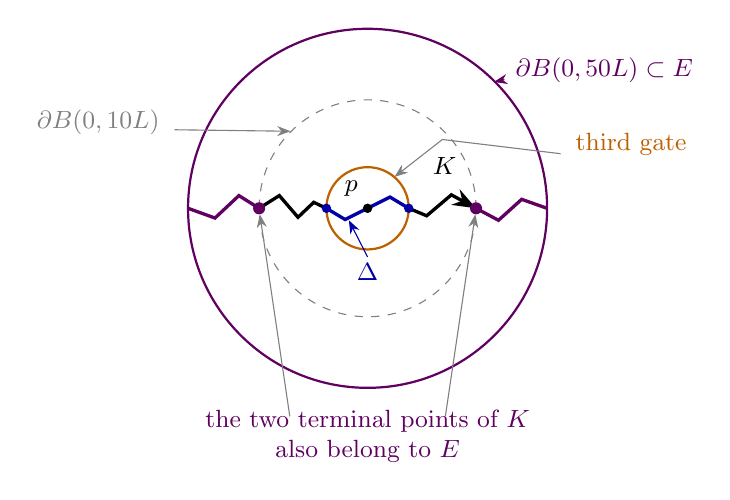
\begin{tikzpicture}[scale=.95,>=Stealth,font=\small]
 \draw[violet!75!black,thick] (0,0) circle (2.4);
 \draw[gray,dashed] (0,0) circle (1.45);
 \draw[orange!75!black,thick] (0,0) circle (.55);
 \draw[very thick] (-1.45,0)--(-1.18,.17)--(-.93,-.12)
       --(-.72,.08)--(-.55,0);
 \draw[very thick,blue!65!black] (-.55,0)--(-.3,-.15)
       --(0,0)--(.3,.15)--(.55,0);
 \draw[very thick,->] (.55,0)--(.79,-.1)--(1.12,.18)--(1.45,0);
 \draw[violet!75!black,very thick] (-1.45,0)--(-1.72,.17)
       --(-2.04,-.13)--(-2.4,0);
 \draw[violet!75!black,very thick] (1.45,0)--(1.75,-.16)
       --(2.06,.12)--(2.4,0);
 \fill[violet!75!black] (-1.45,0) circle (2.3pt)
       (1.45,0) circle (2.3pt);
 \fill[black] (0,0) circle (1.8pt);
 \fill[blue!65!black] (-.55,0) circle (1.8pt)
       (.55,0) circle (1.8pt);
 \node[above left] at (0,.03) {$p$};
 \node[blue!65!black] at (0,-.85) {$\Delta$};
 \draw[->,blue!65!black] (0,-.65)--(-.25,-.16);
 \node at (1.03,.56) {$K$};
 \node[orange!75!black,anchor=west] at (2.65,.85) {third gate};
 \draw[->,gray] (2.58,.73)--(1.0,.92)--(.36,.42);
 \node[gray,anchor=east] at (-2.65,1.15) {$\partial B(0,10L)$};
 \draw[->,gray] (-2.58,1.05)--(-1.03,1.03);
 \node[violet!75!black,anchor=west] at (1.85,1.85)
       {$\partial B(0,50L)\subset E$};
 \draw[->,violet!75!black] (1.83,1.72)--(1.69,1.69);
 \node[violet!75!black,align=center] at (0,-3.05)
       {the two terminal points of $K$\\also belong to $E$};
 \draw[->,gray] (-1.04,-2.78)--(-1.44,-.08);
 \draw[->,gray] (1.04,-2.78)--(1.44,-.08);
\end{tikzpicture}
\caption{A schematic profile in units of $h$, with radial scales not to
scale.  The blue interval $\Delta$ is the part of $K$ inside the third
gate.  The purple set $E$ consists of the complementary rim inside the
outer circle, including the two endpoints of $K$, and the entire outer
circle.  The omitted complementary rim reaches beyond radius $100L$.
Additional excursions are allowed; no smoothness of a profile is assumed.}
\label{fig:pin-profile}
\end{figure}

Fix $\eta_j\downarrow0$, with $\eta_1\le1$.  Choose $\delta_j>0$
successively so small that the following forbidden-return tests have a
summably small total probability.  Two visits in
$\overline B(0,60L)$ at distance at most $\delta_j$ must not have
departures to distance $\eta_j$ along \emph{both} intervening directions
of the rim.  To flag violations use only the local necessary arm events
in Lemma~\ref{lemma:near-return}, on a $\delta_j$-grid inside
$B(0,100L)$, together with the relevant retained-mesh tests.  Their
limiting total probability at level $j$ is at most
\begin{equation}\label{pin:inverse-cost}
 C(L/\delta_j)^2(\delta_j/\eta_j)^{2+c}
       =CL^2\delta_j^c\eta_j^{-2-c}.
\end{equation}
It can be made arbitrarily small.  The events, unlike the profiles
themselves, depend only on this bounded local Poisson restriction.
Only a finite initial list of levels will ever be imposed at a fixed
$h$.

\begin{lemma}[Compactness of profiles]\label{lemma:profile-compactness}
Every sequence of the above profiles satisfying increasingly long
initial lists of the inverse-diameter constraints has a subsequence
converging in marked Fr\'echet and Hausdorff distance to a simple marked
arc $K$ and a compact connected set $E$.  The required marks remain
distinct.  In the limit all visits of $K$ to
$\overline B(0,4b_2)$ occur in the interior of its marked middle interval
$\Delta\subset\overline B(0,b_3)$.  The set $E$ misses
$\overline B(0,4b_2)$ and misses $K\cap B(0,6L)$.
The family of all such limiting profiles is compact.
\end{lemma}

\begin{proof}
The complementary portion of the rim makes a fixed large departure.
Consequently, if two points of $K$ are sufficiently close, the portion
between them in $K$ has small diameter; otherwise both directions would
violate one of the imposed constraints.  More precisely, for a fixed
$j$, closeness at scale $\delta_j$ forces this portion to have diameter
at most $4\eta_j$, after requiring $\delta_j\le\eta_j$.  For tests
initially formulated at vertices, use the buffered test and mesh
smaller than a fixed fraction of each of the finitely many used
$\delta_j$'s to obtain the same implication for points on the polygonal
arc.  The harmless factor four can be absorbed by starting with a
correspondingly smaller sequence $\eta_j$.

Here is a finite-net argument that does not assume length bounds.  Fix
a displacement scale $d>4\eta_j$.  Starting at the first endpoint, stop
successively when the curve first reaches distance $d$ from the preceding
stop, also inserting the marked times.  Apart from a bounded number of
stops adjacent to inserted marks, different stop starts are
$\delta_j$-separated: an intervening displacement $d$ rules out their
closeness by the preceding inverse-diameter property.  Packing in the
fixed disk bounds the number of stops.  Every portion between stops is
contained in a $d$-ball about its start.  Joining the stops by segments
and rounding their positions to a sufficiently fine finite grid gives
a finite marked Fr\'echet net, with error tending to zero as $d\to0$.

Choose a rapidly Cauchy subsequence in these nets and align successive
parametrizations by increasing homeomorphisms matching the marked
times.  The aligned curves converge uniformly to a continuous curve.
If two of its times have the same image, the intervening portion has
arbitrarily small diameter by the inverse constraints, and hence is
constant.  Every point fiber is thus an interval.  Collapse these
constant intervals.  The quotient is a nontrivial compact connected
metrizable linear order, with its order topology: order rays have open
preimages, and compactness identifies the quotient topology.  Such an
order is an interval, as is seen by embedding a countable dense suborder
in an interval and completing the order.  The induced parametrization
is injective and continuous, so the resulting arc is simple.  A
nondecreasing parametrization with constant intervals can be uniformly
approximated by increasing homeomorphisms; with finitely many distinct
marks this can be done separately between consecutive marks.  More
explicitly, after choosing the quotient parametrization so that its
nondecreasing map $q$ fixes the normalized mark times, the maps
$(1-t)q+t\,\mathrm{id}$, $0<t<1$, are increasing homeomorphisms fixing
those times and converge uniformly to $q$.  Thus the
convergence is in the asserted marked Fr\'echet topology.

The radial requirements keep the marks distinct.  For example, if the
ends of $\Delta$ approached one another, the path through the core
would make a fixed departure in one direction and the complementary
path would do so in the other, contradicting an inverse constraint.
The same argument treats the endpoints of $K$ and every pair of
nonadjacent marks; adjacent marks have the radial separation furnished
by the core and the two circles.  In particular the limit is not
constant.

Pass also to a Hausdorff subsequence for $E$.  Connectedness is preserved
under Hausdorff limits of nonempty compact connected sets.  Before the
limit, all visits to $B(0,a_3)$ belong to $\Delta$, and
$a_3>100b_2$; this gives the assertion about
$\overline B(0,4b_2)$ with a margin.  If a complementary-rim point
approached a point of $K$ in $B(0,6L)$, both intervening rim portions
would pass through a terminal hit at radius $10L$.  A fixed
inverse-diameter constraint excludes this approach.  It excludes a
limiting intersection as well.  The added circle at radius $50L$ is
irrelevant in these inner regions.

Finally take any sequence of limiting profiles.  Approximate its $j$th
member closely by a prelimit profile satisfying at least the first $j$
constraints, with the same finite trial data after passing to a
subsequence.  The argument just proved gives a convergent subsequence
of these approximants, and therefore of the limiting profiles.  This
proves compactness of the limiting family.
\end{proof}

\subsection{Models that fit exactly after a small ambient change}

\begin{lemma}[Exact fitting at closed limits]\label{lemma:exact-fit}
Each limiting profile in Lemma~\ref{lemma:profile-compactness} has a
nominal plug model, fixed local stubs, a positive allowed chart-change
tolerance, and an open fit neighborhood with the following properties.
Every fitting prelimit traversal has the strict tracking properties in
Definition~\ref{pin:qualification}.  For every simple profile in the
closure of this neighborhood there is an orientation-preserving ambient
homeomorphism $g$, supported in $B(0,50L)$ and within the allowed
tolerance, such that its ordered arc agrees \emph{exactly} with
$g\Phi(u,0)$ through $gH$ and continues along it to $|u|=9.5$.
There are no other visits of the arc or its unwanted set $E$ to $gH$.
A finite collection of such neighborhoods contains all profiles
satisfying a sufficiently long finite initial list of constraints.
\end{lemma}

\begin{proof}
Extend $K$ to a proper line by outward rays at its two distinct endpoints
on $\partial B(0,10L)$.  The rays are disjoint and meet the closed disk
only at those endpoints.  In the one-point compactification of the
plane, this proper line together with infinity is a Jordan curve on
the sphere.  Apply the sphere Jordan--Schoenflies extension theorem
\cite[Theorems~10.2--10.3, p.~71]{Moise1977} to a correspondence from
the compactified horizontal axis that fixes infinity.  Choose the
correspondence in the given longitudinal order and match the two
complementary sides to preserve orientation.  The extension fixes
infinity and hence restricts to an orientation-preserving plane
homeomorphism $\Psi$ taking the ordered axis to this line.  Prescribe
its longitudinal parametrization in the marked order, with $p$
at $u=0$ and all of $\Delta$ strictly within $|u|<1$.  Assign
$u=-16$ and $u=16$ to the first extensions of $\Delta$ in the
two directions that reach radius $2L$.  The central axis segment
through these parameters lies in $\overline B(0,2L)$; by
continuity, for some $d>0$,
$\Psi([-16-d,16+d]\times\{0\})\subset B(0,3L)$.
This compact segment has positive distance from $E$.  Its parameter
interval contains the chart interval $[-12,12]$, the later cuts
at $u=\pm11$, and their longitudinal buffers.
The rest of the line follows the remaining parts of $K$ and,
beyond its endpoints, the prescribed outward rays to infinity.
Outside the marked middle interval the line misses
$\overline B(0,4b_2)$.

For sufficiently small $\tau>0$, the chart
\[
             \Phi(u,v)=\Psi(u,\tau v),\qquad
             (u,v)\in[-12,12]\times[-3,3],
\]
lies in $B(0,4L)$ and misses $E$; its section at zero is strictly inside
$B(0,a_1)$.  We describe the state and obstacle disks to ensure the
prescribed exact slab intersections.  In straight coordinates take
nested polygonal Jordan neighborhoods approximating the preimages of
the disks of radii $2b_2$ and $3b_2$, inside the preimage of
$B(0,4b_2)$.  They contain the preimage of
$\overline B(0,b_2)$ with a margin and avoid a thin strip about the
axis for $|u|\ge2$.  Adjoin thin horizontal rectangles with longitudinal
intervals $[-3,3]$ and $[-8,8]$, respectively, and fill bounded
complementary components.  The polygons and rectangle widths can be
chosen strictly nested and with transverse intersections of boundaries.
Their unions have connected interiors and disjoint simple polygonal
boundary circuits; filling the holes leaves a single outer boundary.
They are therefore nested Jordan disks.

Choose $3\tau$ smaller than these rectangle half-widths.  Beyond the
specified vertical cuts the remaining thin axis strip escapes to
infinity without meeting either union.  Hole filling consequently
does not change its intersections with this strip.  Their images $O,H$
have precisely the slab intersections $|u|\le3$ and $|u|\le8$ required
in Section~\ref{sec:plugs}.  They miss $E$: before filling they miss
this connected set, which reaches the outer circle, and hence $E$ lies
in the unbounded complementary component.  In physical coordinates
the unions lie in $B(0,6L)$, and their filled hulls remain there because
the exterior of that disk is connected.  Fix stubs and a small positive
chart-change tolerance as in Sections~\ref{sec:plugs} and
\ref{sec:affine}.  Decrease the tolerance to preserve all compact
window margins; in particular nominal coordinates in the terminal
windows change by less than $0.1$.  The support of the ambient change
is allowed inside $B(0,50L)$.

It remains to justify exact fitting, rather than only close tracking.
Consider simple profiles converging to the nominal profile in the
marked topology.  In $\Psi$-coordinates take the subarc from its last
hit of $u=-11$ before the core mark to its first hit of $u=11$ after
the mark.  For close enough profiles this is a proper left-to-right
crosscut of a fixed thin rectangle.  Its interior lies between the
vertical sides, and it stays away from the horizontal sides.
Fr\'echet convergence controls its order and backtracking, so these
crosscuts converge in parametrized boundary distance to the axis
crosscut.

There are homeomorphisms of this rectangle converging uniformly to the
identity that take its midline, in order, to the new crosscuts.  Here
is the extension argument.  Split the rectangle along the old midline
and the new crosscut.  On the boundaries of the two old half-rectangles
prescribe correspondences to the two new halves, using the matching
crosscut parametrizations, the identity on the horizontal sides, and
piecewise linear increasing height maps on the vertical sides.  These
maps agree on the common cut and converge uniformly to the identity.
Each new half is a Jordan domain, and its parametrized boundary
converges uniformly to that of the old half.  Choose a fixed interior
point of each old half, which belongs to every sufficiently close new
half, and normalize the conformal maps at that point with positive
derivative.  Rad\'o's uniform convergence theorem for Jordan domains
with Fr\'echet-convergent boundaries
\cite[\S\S1--2, pp.~182--183]{Rado1923} gives convergence of these
maps on the closed disk.  Write them as $F_n,F$, and write $h_n$ for
the prescribed boundary correspondence.  The circle homeomorphisms
$\chi_n=F_n^{-1}h_nF$ converge uniformly to the identity: for
$\zeta\in\partial\mathbb D$,
\[
 |F(\chi_n(\zeta))-F(\zeta)|
       \le\|F_n-F\|_\infty+\|h_n-\mathrm{id}\|_\infty,
\]
and the inverse of the fixed closed Jordan chart $F$ is uniformly
continuous.  Extend these circle homeomorphisms radially by
$re^{\ii\theta}\mapsto r\chi(e^{\ii\theta})$; these are disk
homeomorphisms with the same uniform convergence.  Conjugation by the
conformal charts gives the desired half-rectangle homeomorphisms,
with the prescribed exact values on the common cut and uniform
convergence to the identity.  The cut parametrizations can match all
three interior marks: interpolate the small changes of their terminal
parameters by increasing piecewise linear maps fixing those marks.
Glue them along the cut.  Interpolate the small vertical-side height
changes to the identity in thin exterior collars, keeping the top and
bottom fixed.  The result extends by the identity to a plane
homeomorphism.  After conjugating by $\Psi$, its support can be kept in
$B(0,50L)$ and its displacement tends uniformly to zero.

The portions of the ordered arc omitted by this crosscut correspond,
for close enough profiles, to nominal axis positions with
$|u|>10.5$.  The original compact margins separate them from the changed
obstacle and the central track through $|u|\le9.5$.  The unwanted set
$E$ is separated there as well.  Thus every sufficiently close simple
profile admits the required change within any prescribed positive
tolerance.  First obtain this conclusion on a neighborhood, and then
choose a smaller neighborhood whose closure among simple profiles is
contained in it.  This gives the stated closed-limit property and the
strict prelimit tracking requirements.

Cover the compact family of limiting profiles by finitely many such
open neighborhoods.  If no finite initial constraint list forced
membership in their union, one could choose a profile outside the
union satisfying the first $j$ constraints for every $j$.
Lemma~\ref{lemma:profile-compactness} would give a subsequential limit
inside the union, contradicting openness.  Thus one finite list
suffices.  The construction uses only normalized profile geometry and
the finite trial data, so the same finite menu works at every
sufficiently small $h$.
\end{proof}

On fine retained mesh a fitting traversal supplies vertices near
$u=\pm1.7$ joined along that rim within
$\Phi([-2,2]\times I_B)$, and supplies both side passages in the
nominal windows.  The transverse and backtracking margins, rather than
a smoothness or transversality assumption on the rim, give these
conclusions.  All visits near the second gate annulus belong to
$\Delta$.

\subsection{Local preparations, ranks, and propensities}

For each of the finitely many chart and color choices at a grid center,
apply a separate preparation to the original points and colors.  In
the black case it acts only in a narrow substrip of
$\Phi([-7.5,7.5]\times I_W)$.  It forces a retained white walk from
about $u=-7.1$ to $u=7.1$ with longitudinal backtracking less than $0.2$.
Choose a buffered chain of crossing rectangles along the substrip,
using overlapping progress steps whose chart-longitudinal widths are
much smaller than $0.2$.  Crossings in both directions in the overlaps
join the successive walks.  They can be concatenated in order, with
the desired width and progress margins, through both side-test
terminals.  The corridor argument of Section~\ref{sec:plugs} and the
quenched rectangle bounds give, on a local geometry event with
probability tending to one, a conditional success probability at least
$p_*>0$.  Since there are finitely many normalized models, take a
common positive lower bound.  The good event can be the retained-mesh
event and this lower-propensity event itself.

The preparation uses the finite ordered-coupling principle; see
\cite[Theorem~4.1 and its finite-network discussion]{Edwards1978}.
For completeness, the finite-spin construction needed here is as follows.  If $A$ is increasing under the white order for a finite
product measure $\pi$, positive association implies
$\pi(B\mid A)\ge\pi(B)$ for every increasing set $B$.
There is therefore a coupling $(\omega,\omega')$ with laws
$\pi,\pi(\cdot\mid A)$ and $\omega\le\omega'$.
One may obtain it by a finite flow network: supply $\pi(\omega)$ at
each initial state, demand $\pi(\omega'\mid A)$ at each final state,
and allow an edge exactly when $\omega\le\omega'$.  The inequalities
for increasing sets are precisely the cut inequalities, and the
max-flow criterion supplies the coupling.  Its conditional transition
law is a kernel that only recolors existing black sites white,
with the point geometry fixed.  Fix a deterministic choice of
flow for each finite ordered truth table and probabilities; this also
ensures measurability when the point configuration varies.  Each
bounded local region contains finitely many sites almost surely.

Activate this kernel solely according to its local geometry event,
using an independent seed, and otherwise do nothing and flag the
location.  In particular its activation does not condition on a
fitting rim.  Given the geometry its output law is bounded by
$\max(1,p_*^{-1})$ times ordinary spinning.  Writing
$\sigma^{\mathrm{prep}}$ for the full prepared coloring, its joint
law with the unchanged point configuration consequently satisfies
\[
 \mathcal L(\eta,\sigma^{\mathrm{prep}})
                 \le \max(1,p_*^{-1})\nu,
\]
as measures, uniformly in $h$.
Different candidate outputs need not have a jointly dominated law;
we use the bound for each individual preparation, and for two
disjoint preparations with independent seeds.  The flipped construction
recolors existing white sites black in the opposing strip for white rims,
again fixing the point geometry.

At a fit the preparation avoids the rim.  It keeps both gate circuits
with at most two black vertices and supplies a single white traversal
whose root portion and side portions are compatible.  Together with
the original black traversal, some pair of root ranks therefore has
both side successes.  The ranks can be truncated uniformly with
arbitrarily small error.  Indeed distinct crossing components of a
root window supply vertex-disjoint same-color paths across its middle
slab.  On good geometry an opposing transverse bar has quenched
probability at least $q>0$.  Thus the probability of one such
monochromatic crossing is at most $1-q$, and the conditional BK
inequality bounds the probability of $k$ disjoint crossings by
$(1-q)^k$.  Transfer this bound to the prepared output using its
density bound, and discard the negligible geometry failure.  A fixed
large rank cutoff works for the finite collection of windows.

We next discard actual successes whose ordinary conditional
propensities are too small.  For any event $A$ and sigma field
$\mathcal F$,
\begin{equation}\label{pin:small-propensity}
 \nu\bigl(A\cap\{\nu(A\mid\mathcal F)<t\}\bigr)
 =\EE_\nu\bigl[\ind_{\{\nu(A\mid\mathcal F)<t\}}
                 \nu(A\mid\mathcal F)\bigr]\le t.
\end{equation}
Apply this first to $L^+$ and $L^-$ conditional on the inner state,
and then to each white side success conditional also on the local
exterior point geometry.  Transfer each estimate by the preparation
density and take a finite union over the retained ranks and models.
Choosing $\beta>0$ small makes the total cost arbitrarily small.
Finally, for each resulting type discard its actual prepared
occurrence of $G$ when $\nu(G)<\beta'$.  Its probability is at most
$C\beta'$ per type.  Choose $\beta'>0$ after the finite rank
truncation.  The remaining prepared states have exactly the
qualifications in Definition~\ref{pin:qualification}.

All discard flags are local.  A side-test propensity conditional on the
inner state is a measurable function of that state and fixed local
test; its quenched counterpart additionally uses only the exterior
point restriction needed by its retained paths.  The preparations,
rank counts, actual side successes, and admission indicators use no
hypothetical long connector.  Their range is bounded by $CL$ in
normalized units.  Stubs are not queried by these flags.

\subsection{From rare flags to dense pins}

\begin{proposition}[Density of qualified pins]\label{prop:dense-pins}
There exist a finite normalized menu and fixed $\beta,\beta'>0$ such
that the following holds in every bulk patch with
$\overline B(x,6R)$ available.  With probability tending to one in the
ordered limit $\eps\to0$, then $h\to0$, every subarc of diameter at
least $r_h$ in $\overline B(x,2R)$ on a rim reaching outside
$B(x,4R)$ contains a qualified pin.  The statement holds simultaneously
for all such subarcs and both colors.  It also holds for the coupled
bulk settings on their patch-agreement event.
\end{proposition}

\begin{proof}
For either color, the preceding local tests have the following
deterministic implication on patch agreement and good mesh: every
eligible marked rim vertex within distance one of a grid center fits
some qualified choice unless that center is flagged.  The trial part
of its limiting flag probability is \eqref{pin:trials}.  For fixed $L$
all other costs can be made arbitrarily small.  The order of choices is
essential.  Choose $M,n$ first.  Allocate a summable inverse-test budget,
which determines the finite profile menu and its finite constraint
list.  For that menu fix the preparation corridors and their positive
lower bounds, then truncate ranks, and finally choose the two
propensity thresholds.  Every choice is in normalized units and
independent of $h$.  Admission itself need not stabilize here.

Tile the plane by blocks of side $Lh$.  A block is bad if its enlargement
by distance $2Lh$ contains at least $c_0L$ flagged grid centers, where
$c_0>0$ is a sufficiently small absolute constant.  There are $O(L^2)$
candidate centers in that enlargement, so the first-moment bound gives
\begin{equation}\label{pin:flag}
 \limsup_{\eps\to0}\PP(\text{a specified block is bad})
 \le CL\bigl[Cn^2(CM^{-1-c})^{n-2}+\zeta\bigr],
\end{equation}
where $\zeta$ is the sum of the adjustable additional costs.  Since
$L=30M(10^4M)^{n-1}$, first taking $M$ large and then $n$ large makes
the contribution $L n^2(CM^{-1-c})^{n-2}$ as small as desired.
Choose $\zeta$ afterward.  The dependence range of these block events
is an absolute constant in block units, including the independently
assigned preparation seeds.

An eligible subarc of diameter at least $r_h$ without a qualified pin
forces a connected chain of bad blocks of length at least
$c r_h/(Lh)$.  Choose two points of the subarc at distance at least
$r_h/2$ and follow the portion between them.  Since $r_h/(Lh)\to\infty$,
at least one of these endpoints lies outside the $2Lh$ enlargement of
each visited block.  From a visit to the block, follow the subarc toward
that endpoint until it first leaves the enlargement.  Even if the visit
only clips a corner of the block, this portion travels distance at least
$2Lh$.  On fine mesh, its initial passage over distance $Lh$ supplies
vertices within distance $h$ of at least $c_0L$ distinct grid centers,
all still inside the enlargement.  Every such center is flagged by the
deterministic implication above.  Thus every visited block is bad.
The visited blocks connect the two chosen endpoints; erasing repetitions
gives a chain of distinct neighboring bad blocks, whose length is at
least $c r_h/(Lh)$ by their separation.

There are exponentially many block chains of a specified length, and
only $O(h^{-2})$ possible starting blocks in the fixed patch.  From any
chain of length $k$ choose at least $k/C_0$ blocks whose flag-data
regions are pairwise disjoint.  Their bad events are independent under
the full-plane marked Poisson law with the local seeds.  If the bound
in \eqref{pin:flag} is sufficiently small, exponential path counting
therefore gives an upper bound of the form
\[
          C_Rh^{-2}\exp\{-c r_h/(Lh)\}\longrightarrow0.
\]
At each fixed $h$ the chain length and all local scale lists are finite;
take the microscopic limit before this estimate.  Discarding the
vanishing patch-agreement and mesh failures completes the proof.
\end{proof}

\section{Transport along actual arcs}\label{sec:actual-arcs}

We first transfer the fixed-connector rule to arcs in the original random
configuration, retaining their assigned prepared endpoint states. We
then pass from arc contributions to smooth weights. The second step
requires a separate control of signed sums and completes bulk transport.

Fix a countable sequence $h\downarrow0$.  Starting with any microscopic
sequence, make the subsequence choices of Section~\ref{sec:affine}
simultaneously for these $h$'s.  The grid translates of the menu, their
representatives, and their integer winding classes form countable lists;
admissions can be stabilized for each $h$ because there are finitely many
types.  All microscopic limits below are taken on this one further
subsequence.  In particular the scalars $a_h^Q$ are bounded uniformly in
$h$ and $a_h^V=1$.  Comparisons involving an empty set of admitted types
are vacuous.

We continue to work in a bulk patch containing $\overline B(x,6R)$.
Every qualified pin is used with a specified fitting test, type, ranks,
and the prepared state assigned in Section~\ref{sec:pins}.  No
comparison below changes that assigned state.

For two ordered pins $s,t$ on $P$, write
$D_s=B_s=\overline B(z_s,m_sh)$ for the previously defined placed
cutoff ball at $s$, and similarly $D_t=B_t$ at $t$. Define
\[
 I_X(P;s,t)
   =X_P(\ind_{D_s})
     +\sum_{\substack{e\text{ on the forward arc }p_s\to p_t\\
               \text{right tag of }e\notin D_s\cup D_t}}
                   X_P(e),\qquad X\in\{Q,V\}.
\]
Here $X_P(e)$ denotes the contribution of the oriented edge with its
right tagged triangle.  The first term is the \emph{entire} start
cutoff mass, not only the portion after $p_s$.  This convention will
make concatenation exact.

\subsection{Two conditional-measure and locality facts}

\begin{lemma}[A dominated forcing kernel]\label{lemma:dominated-kernel}
Let $\nu$ be a probability measure on configurations, let $Z$ be
retained data, and let $\nu_z$ be a regular conditional law given $Z=z$.
Suppose $H$ is a measurable set of retained data and
$p(z)=\nu_z(W)\ge q>0$ on $H$.  Let $K$ fix $Z$ and satisfy
$\nu_zK_z=\nu_z(\cdot\mid W)$ there.  If an unnormalized
subprobability $\lambda$ satisfies $\lambda\le C\nu$ and is supported
over $H$, then
\[
                         \lambda K\le (C/q)\nu.
\]
For the additional monotone assertion, suppose that, conditional on
$Z=z$, the remaining coordinates have law
$\nu_z=\pi_z\otimes\tau_z$, where $\pi_z$ is a product spin law on
a finite, $Z$-measurable set $I(z)$ of exterior sites and $\tau_z$
is the law of the complementary data. Suppose also that $W$ depends
only on $Z$ and the spins in $I(Z)$ and is increasing in white on
those spins. Then $K$ can be chosen to recolor only existing black
sites in $I(Z)$ white and to fix $Z$ and every complementary coordinate.
\end{lemma}

\begin{proof}
For every nonnegative measurable function $g$, positivity of a kernel
and disintegration give
\begin{align*}
 \int\lambda(\dd\omega)Kg(\omega)
 &\le C\int\ind_H(Z(\omega))\nu(\dd\omega)Kg(\omega)\\
 &=C\int_H\nu^Z(\dd z)\,
       \frac{1}{p(z)}\int\ind_W(\omega')g(\omega')
                                      \nu_z(\dd\omega')\\
 &\le(C/q)\int g\,\dd\nu.
\end{align*}
No assumption is made about the conditional law of $\lambda$ given
$Z$. Under the additional hypothesis, association of $\pi_z$ shows
that $\pi_z(\cdot\mid W)$ stochastically dominates $\pi_z$ in the
white order. The finite ordered coupling construction in
Section~\ref{sec:pins}, applied on each retained-data fiber, gives
a measurable white-adding kernel for this block. Independence of
the complementary data lets us use the identity there: the output
law is $\pi_z(\cdot\mid W)\otimes\tau_z=\nu_z(\cdot\mid W)$.
\end{proof}

\par\ifdim\dimexpr\pagegoal-\pagetotal\relax<6\baselineskip\newpage\fi
\begin{lemma}[Retention with collars]\label{lemma:retained-collar}
Fix $h$ and finitely many deterministic path envelopes and state disks.
Suppose the point data are kept on a deterministic Borel set containing
an open collar of every envelope and of the state portions under
comparison.  Set $\rho_\eps=\sqrt{h\eps}$.  For small $\eps$, every
Delaunay triangle of circumradius at most $\rho_\eps$ meeting these
envelopes, together with its incident edge and tag data there, is
determined by the kept point restriction.  Thus two configurations
with the same restriction have the same such local triangulations.

In a fixed two-plug comparison one can keep the two endpoint states and
the whole exterior sector of the used connector.  The inset paths of
the cycle experiment and any sufficiently closely tracking actual
arc, including their inner second-gate paths, then have the common
triangulations just described on the ordinary mesh-good events.  The
complementary connector can be resampled without altering them.
\end{lemma}

\begin{proof}
A Delaunay triangle is determined by its three vertices and emptiness
of its circumdisk, apart from the null degeneracies excluded in our
model.  If its circumradius is at most $\rho_\eps$ and it meets a fixed
envelope, its circumdisk lies within a constant multiple of
$\rho_\eps$ of that envelope.  This is eventually inside its kept
collar.  The same observation determines all retained triangles
incident to its local edges.  On mesh-good events all triangles
needed for the ordinary local paths and their right tags satisfy this
bound, by Lemma~\ref{lemma:mesh}.  This proves the first assertion
without any assumption on the area of the boundaries of the kept
sets.

For the second assertion, the paths in the cycle experiment lie in
fixed inset layers of the embedded annular band.  Outside states these
layers, the tube-test footprints, and the joining seams have positive
margins to the lateral boundaries of the used sector.  Inside states,
the relevant second-gate paths and cutoff triangles lie in a compact
subset of $O$, since the gate annuli and cutoff balls have the
prescribed radial margins.  The same envelopes contain the actual
paths when the track fit is sufficiently close.  Their exterior
portions and state portions therefore have collars within the kept
union, as also in Lemma~\ref{lemma:fixed-collar}.  The other sector
queries disjoint exterior restrictions.  Deterministic Borel
allocation of boundaries suffices; no smooth-boundary convention is
needed.  The first assertion now applies in both configurations.
\end{proof}

\subsection{Winding and a finite deterministic family of comparisons}

\begin{lemma}[Winding bound]\label{lemma:winding}
Except on events of probability tending to zero in the ordered limit,
every subarc of a rim in $B(x,3R)$ that stays at distance at least $h$
from a grid center in use has absolute net change of continuous
argument about that center at most
$C_R(1+|\log h|^2)$.
\end{lemma}

\begin{proof}
Fix a ray from the center and divide its relevant distances into
dyadic bins $d\asymp 2^jh$, up to scale $O(R)$.  In each bin a bounded
number of balls of radius a small fixed fraction of $d$ cover possible
ray passages.  Give each ball a buffered outer ball of comparable
radius, all within the bulk patch.  A passage off the ray followed
by a quarter turn leaves one of these outer balls, and so gives a
monochromatic crossing of its fixed-ratio annulus.  Successive full
turns contributing to a net argument change can be selected by first
hits of successive levels of a lifted argument.  Their portions
between the relevant passage and departure times are disjoint on the
simple rim; trimming with the fixed margins yields vertex-disjoint
annular crossings on fine mesh.

On crossing-good geometry an opposite-color circuit in such a test
annulus has probability at least a fixed $q>0$.  Hence one
monochromatic crossing has probability at most $1-q$, and conditional
BK bounds the probability of $k$ disjoint crossings by $(1-q)^k$.
There are $O_R(h^{-2})$ centers and $O(1+|\log h|)$ bins per center.
At each fixed $h$ the geometry exceptions for this finite list vanish
as $\eps\to0$.  A union bound with
$k=C_R(1+|\log h|)$ leaves probability tending to zero as $h\to0$.
Summing over the bins bounds the net number of turns by
$C_R(1+|\log h|^2)$, and the incomplete initial and final turns add
only a constant.
\end{proof}

Fix $h$ for the moment and an arbitrarily small probability budget
$\zeta>0$.  Impose the local inverse-diameter tests from
Section~\ref{sec:pins} throughout $\overline B(x,3R)$, to a finite
number of accuracy levels to be chosen below, at total limiting cost
less than $\zeta$.  Track a qualified arc from $s$ to $t$ together
with its extension from the start of $K_s$ to the end of $K_t$, saving
both marked endpoint profiles.  Assume the original arc lies in
$\overline B(x,2R)$, $|z_s-z_t|\ge R/3$, and its complementary rim
reaches outside $B(x,4R)$.  For small $h$ the endpoint neighborhoods
of size $10Lh$ are disjoint and occur in the required order, so the
extended arc lies in $B(x,5R/2)$ and its complement still makes a
fixed large departure.

The proof of Lemma~\ref{lemma:profile-compactness}, in this fixed
physical region, applies to these extended marked arcs.  Along
sequences satisfying increasingly many constraints it gives simple
Fr\'echet limits, simultaneously with their endpoint profile limits.
At fixed $h$ the placements, templates, and retained ranks lie in
finite lists.  Pass to fixed choices.  The endpoint limits are in the
closures of their assigned fit neighborhoods.  A visit near an end
obstacle not belonging to its prescribed $K$ is included in that
profile's $E$: the relevant neighborhood is well inside the radius
$50Lh$ truncation.

Lemma~\ref{lemma:exact-fit} supplies independently supported permitted
changes of the two end charts, making the limiting extended arc the
exact centerline through both changed obstacles and for a further
collar on either side.  It avoids the obstacles elsewhere.  The
band-and-collar construction of Section~\ref{sec:plugs} now fits a
connector to the intervening simple arc, with the full prescribed
port sections, inside the bulk patch.  A complementary connector
exists in the plane; it need not lie in the patch.  The two-twist
classification applies: a net argument along a limiting arc separated
from a center persists under close Fr\'echet approximation.  Thus
Lemma~\ref{lemma:winding} bounds the two winding integers by
$C_R(1+|\log h|^2)$, up to a bounded contribution from the fixed stubs
and allowed chart changes.  Since $|z_s-z_t|/h\ge R/(3h)$, the
distance requirement in Proposition~\ref{prop:endpoint-potentials}
holds for small $h$.

This fixed connector works on an open neighborhood of the limiting
track data.  In particular the actual root vertices near nominal
$u_s=1.7$ and $u_t=-1.7$ are joined by the actual rim within its
black tube.  The corresponding compact portion of the limiting
centerline is interior to that tube and is well beyond the
longitudinal cutoffs $u_s=0.5$ and $u_t=-0.5$.  Small allowed chart
changes preserve the nominal root positions and windows.  The
product-band seams are interior, so a sufficiently close ordered fit
and fine mesh preserve all these margins, including retention of the
required paths.

There is a further gate-order issue.  Use the first and second
circuits selected from the prepared states.  Every contact with the
actual rim lies on its isolated central traversal and remains black
after preparation.  Each selected circuit has at most two black
vertices in that prepared state, so it has at most two contacts with
the original rim.  Passage from inside to outside requires two;
there are therefore exactly two contacts, traversed once.  This
argument applies even if a selected circuit differs from the
original gate choice.  A full chart slab about
zero lies in the inner gate ball.  The limiting track enters this
slab from the negative side and leaves on the positive side; its
contacts with a surrounding gate lie away from the slab.  On a
sufficiently close ordered fit their signs cannot change.  Thus the
first exit at $s$ and the first entry at $t$ are the designated
positive and negative gates.  The intervening path remains in the
used sector, with room in its interior together with the endpoint
states, and avoids the opposing layer.  It cannot recross a central
section while outside the corresponding first gate.  The inner
second-gate paths also track the local centerline inside their
states.  This argument uses the progress through a slab, not a
transversal crossing of a discrete edge with a curve, and is uniform
over the possible locations of the circuits in their annuli.

Compactness and the finite-list argument in
Lemma~\ref{lemma:exact-fit} now give a finite family of these
deterministic patterns whose open neighborhoods cover all tracks
satisfying a sufficiently long finite constraint list and the winding
bound.  Patterns are chosen from limiting deterministic track data
before the random comparison; a new band is not selected after
observing the colors.  Only finitely many placed patterns, endpoint
types, and rank choices occur at this fixed $h$.  The open track
tests and existential path conditions are measurable: graph paths
are countable given the locally finite graph, and the marked fits
use the usual Fr\'echet open sets.

\subsection{The comparison with a cycle experiment}

\begin{proposition}[Transport on a real arc]\label{prop:real-arc}
Simultaneously for $X=Q,V$ and every qualified ordered arc from $s$
to $t$ contained in $\overline B(x,2R)$, with
$|z_s-z_t|\ge R/3$ and complementary rim reaching outside
$B(x,4R)$, one has
\begin{equation}\label{actual:arc}
 \left|I_X(P;s,t)-a_h^X(z_t-z_s)
       -\phi_s^{X,+}(\sigma'_s)-\phi_t^{X,-}(\sigma'_t)\right|
       \le C_Rh(1+|\log h|^2)
\end{equation}
outside events whose probability tends to zero in the ordered limit.
The constant is independent of the complexity and conditioning
constants of the individual fixed comparison patterns.
\end{proposition}

\begin{proof}
We construct one comparison for all qualifying arcs of each pattern
in the finite deterministic cover.  Write $\xi$ for the original input,
with law $\mathsf P$, including the bulk/full-plane coupling and all
assigned local preparation seeds.  Let $E_0$ be the common input event
on which patch agreement and the covering and winding conclusions hold,
intersected with
the original mesh and continuation-geometry conditions of all patterns.
These additional conditions have total failure probability $o(1)$ at
fixed $h$.  The covering exception will be paid once, through
$\mathsf P(E_0^c)$.

Fix a placed connector $e:s\to t$, a complementary connector $c$, and
their endpoint choices.  Let $\mathscr C_e(\xi)$ be the collection of
all qualifying ordered rim arcs of this pattern, including their assigned
preparation outcomes.  Put
\[
 A_e=\{\mathscr C_e(\xi)\ne\varnothing\},\qquad A_{e,0}=A_e\cap E_0.
\]
We retain the original input throughout and work with the
\emph{unnormalized} restriction $\mathsf P|_{A_{e,0}}$; its mass is
never divided by the probability of a fit.  We describe the construction
for black arcs; for white arcs exchange the colors.

\paragraph{Prepare the endpoints and force the white connection.}
Let $F_e(\xi)$ be the underlying plane configuration after the two
specified local white-adding preparations, with their already assigned
seeds.  Their supports are disjoint.  Before restriction, independence
of the seeds conditional on geometry and the local preparation bounds
give a configuration marginal bounded by $C_{\rm prep}\nu$.  Hence
\[
 \lambda:=F_{e*}(\mathsf P|_{A_{e,0}})\le C_{\rm prep}\nu.
\]
Restriction only deletes mass, even when it inspects actual arcs,
other preparations, seeds, and patch data.  The endpoint states of
$F_e(\xi)$ are precisely the assigned $\sigma'_s(\xi),\sigma'_t(\xi)$.

Define $Z$ on the ordinary configuration space to be the coordinate
map consisting of the full point geometry $\eta$ and the colored
configuration restrictions to the two state regions $O_s,O_t$.
On a prepared output these last two coordinates have the assigned
values $\sigma'_s,\sigma'_t$. Thus $\nu(\cdot\mid Z)$ refers to
ordinary coordinate restrictions, not to conditioning on the outcome
of a preparation algorithm under its input law. Let $W$ be the white
part of $S_e$. Under the ordinary law conditional on $Z$, the exterior
colors are independent fair bits. Each needed white side event has probability at least
$\beta$ by qualification.  These two endpoint events use disjoint
exterior bits.  The white continuation network uses the buffered
exterior corridors of Lemma~\ref{lemma:bridge}.  On its good point
geometry, association in the white order therefore gives
\begin{equation}\label{actual:quenched-force}
                  \nu(W\mid Z)\ge q_{\rm cont}\beta^2=:q_0>0.
\end{equation}
The local qualification is unchanged by additionally conditioning on
the rest of $\eta$, since its retained side tests query only their
specified local point restrictions.  The continuation-geometry conditions
were included in $E_0$ and have vanishing failure probability; the
preparations keep the point geometry fixed.

Let $H$ be the resulting set of $Z$ values on which
\eqref{actual:quenched-force} holds. For this fixed pattern let
$I=I(\eta)$ contain \emph{all potential exterior sites} in its
buffered white footprint on which $W$ can depend. This finite block
is selected from the geometry before colors or witnesses are inspected;
it is not an adaptive query transcript. Every site in it is separated
from the permitted black track layer. Conditional on $Z$, its fair
product spin law is independent of all complementary exterior spins,
and $W$ depends only on $Z$ and this block. Equivalently, with
$\widetilde Z=(Z,\sigma_{\rm ext\setminus I})$, these spins remain
independent fair bits and
$\nu(W\mid\widetilde Z)=\nu(W\mid Z)\ge q_0$ over $H$.
The monotone clause of Lemma~\ref{lemma:dominated-kernel} therefore
applies to $\lambda$, which is supported over $H$. Use its kernel
$K_e^W$ to add white only in $I$, fixing every other
coordinate. The lemma yields
\[
                 \lambda K_e^W\le(C_{\rm prep}/q_0)\nu.
\]
This conclusion does not assume that the selected input has ordinary
conditional exterior spins.  Its conditional law may be arbitrary;
the subprobability domination is what permits the forcing.  The
kernel only removes black sites in the separated white footprint.
It preserves every track in $\mathscr C_e(\xi)$, with its buffered
collars and fixed states.  Thus the output satisfies $S_e$.

\paragraph{Complete the configuration while retaining the used sector.}
Keep the endpoint states and the whole exterior $e$-sector datum,
denoted together by $M_e$.  Under the ordinary kept-data law
$\nu_{M_e}$, the corresponding marginal $\rho_{M_e}$ of the
two-plug cycle experiment has density
\begin{equation}\label{actual:cycle-density}
 \frac{\dd\rho_{M_e}}{\dd\nu_{M_e}}
 =\frac{\ind_{G_s}\ind_{G_t}\ind_{S_e}}
 {\nu(G_s)\nu(G_t)\nu(S_e\mid\sigma'_s,\sigma'_t)}.
\end{equation}
The denominator is positive by admission and \eqref{plug:success},
and is at most one.  The post-forcing marginal is supported on the
three events in the numerator and dominated by
$(C_{\rm prep}/q_0)\nu_{M_e}$; it is therefore dominated by
$(C_{\rm prep}/q_0)\rho_{M_e}$.  Apply to both
measures the same completion kernel: sample the other exterior
connector region, geometry and colors, conditional on $S_c$ and the
two states, and sample the remaining plane ordinarily.  This keeps
$M_e$ and the collars of the compared paths unchanged.  Denote the
composition of $K_e^W$ with this completion kernel by $\mathcal K_e$,
extending it arbitrarily off the relevant support.  On the original
input and final configuration together, define
\[
 \Pi_e(\dd\xi,\dd\omega')
   =\ind_{A_{e,0}}(\xi)\mathsf P(\dd\xi)
             \mathcal K_e(F_e(\xi),\dd\omega').
\]
Its input marginal is exactly $\mathsf P|_{A_{e,0}}$.  The construction
gives the two properties needed below:
\[
 \begin{aligned}
 &(\operatorname{pr}_{\rm out})_*\Pi_e\le D_e\rho_e,\\
 &(\sigma_s(\omega'),\sigma_t(\omega'))
       =(\sigma'_s(\xi),\sigma'_t(\xi))
       \quad\Pi_e\text{-almost surely}.
 \end{aligned}
\]
Here $\rho_e$ is the two-plug cycle law and $D_e<\infty$ is fixed
at fixed $h$ and pattern.  The first follows by applying the same
completion kernel to the dominated kept-data marginals; the second
holds because both kernels fix the endpoint states.  No product
domination of the joint law is required.

\paragraph{Compare every fitting arc to one output rim.}
Choose one experiment rim $P'_e=P'_e(\omega')$ by a measurable
rule depending only on the output.  There is one event
$\mathcal G_e$ in this joint space, independent of a choice of
$\gamma\in\mathscr C_e(\xi)$, such that
$\Pi_e(\mathcal G_e^c)=o(1)$ and the following path comparisons
hold.  Use the mesh and shielding conditions on the deterministic
state and sector envelopes in both configurations, and the
mesh conditions for the confined cycle-rim construction.
Their original failure mass is bounded by the original mesh
probability; their final failure mass is bounded by $D_e$ times
the cycle mesh probability.  The strict track and gate-order
margins hold for every member of $\mathscr C_e(\xi)$ by the one
fixed pattern's fit test.  Thus the good event and the output
kernel are not chosen separately for different arcs.

On $\mathcal G_e$, the first-exit to first-entry path of $P'_e$
and its inner second-gate paths are black in the original graph.
Colors only changed from black to white before completion,
and completion resamples outside their kept envelopes.
Conversely, the corresponding portions of every input arc in
$\mathscr C_e(\xi)$ remain black in the final graph: the
preparations and white forcing avoid their permitted track layer,
and completion keeps the whole used sector and endpoint states.
Lemma~\ref{lemma:retained-collar} gives the common complete
incident triangulations and gate fans. Since $b_2<a_3$, the first
and second gates lie strictly inside the unchanged third circuit.
Third-gate isolation puts every original-rim contact with a gate selected from the
prepared state on the untouched central traversal.  The selected
gate has at most two path-color vertices, while each fitting rim
visits both sides, so every such rim uses precisely those two
contacts.  The output rim does too, and ordered passage through
the central slab gives the same signs; this also covers a selected
gate differing from the originally exhibited gate.
Lemma~\ref{lemma:gate-consistency} now
identifies the inner second-gate paths and the outside path,
using the inside and outside starting fans, respectively.
At a first divergence a mutually black compared path would give
a forbidden bypass up to its first subsequent contact with the
whole other rim.  This argument applies in each graph separately
and to every input arc with the same $P'_e(\omega')$; the original
rim need not remain a complete rim after modification.

Set
\[
 H_e^X(\omega')
  =\widehat m_s(P'_e(\omega'))+\widehat j_e(P'_e(\omega')),
                           \qquad X=Q,V.
\]
All cutoff tags belong to the common inner second-gate paths.
The marks and inner first-gate paths lie inside the cutoffs, and
the outside-cutoff mass lies on the common outside path.  Thus
on the same event $\mathcal G_e$,
\begin{equation}\label{actual:exact-comparison}
 I_X(\gamma;\xi)=H_e^X(\omega')
 \quad\text{for all }\gamma\in\mathscr C_e(\xi),\qquad X=Q,V,
\end{equation}
where $I_X(\gamma;\xi)$ is the original $I_X(P;s,t)$.
In particular the right side is one output random variable,
not a separately coupled variable for each input arc.

\paragraph{Return the estimate to the original input.}
For endpoint states $\sigma=(\sigma_s,\sigma_t)$ write
\[
 \Theta_e^X(\sigma)=a_h^X(z_t-z_s)
        +\phi_s^{X,+}(\sigma_s)+\phi_t^{X,-}(\sigma_t).
\]
Separate the cycle-mass error from the retained-state remainder:
\[
 \begin{aligned}
 C_e^\eps(\omega')
   &=\max_X|H_e^X(\omega')
               -i_e^\eps(\sigma_s(\omega'),\sigma_t(\omega'))|,\\
 R_e^\eps(\sigma)
   &=\max_X|i_e^\eps(\sigma)-\Theta_e^X(\sigma)-b_e^{X,\eps}|.
 \end{aligned}
\]
Here $i_e^\eps$ in each term is the function for field $X$, and
$b_e^{X,\eps}$ is its deterministic bias.
Equations~\eqref{plug:cycle} and \eqref{affine:transport} give
\[
 \EE_{\rho_e}C_e^\eps=o(1),\qquad
 \EE_{\mu_s\otimes\mu_t}R_e^\eps=o(1).
\]
The input law of its two prepared states, restricted to
$A_{e,0}$, is bounded by $C_{\rm prep}\mu_s\otimes\mu_t$.
Indeed the endpoint marginal of $\lambda$ is bounded by
$C_{\rm prep}$ times the independent ordinary state product and is supported on
$G_s\cap G_t$; restricting that product gives
$\nu(G_s)\nu(G_t)\mu_s\otimes\mu_t\le\mu_s\otimes\mu_t$.
The pathwise retained-state equality makes
$\Theta_e^X(\sigma'_s(\xi),\sigma'_t(\xi))$ exactly the target
computed from the output states.

Let $B_e^\eps=\max_X|b_e^{X,\eps}|$ and fix $u>0$.
On $\mathcal G_e$ the error of every fitting input arc is at most
\[
 B_e^\eps+C_e^\eps(\omega')
             +R_e^\eps(\sigma'_s(\xi),\sigma'_t(\xi)).
\]
Consequently the original-input probability, restricted to
$A_{e,0}$, that any such arc has error greater than
$B_e^\eps+2u$ is at most
\[
 \Pi_e(\mathcal G_e^c)
 +D_e\rho_e(C_e^\eps>u)
 +C_{\rm prep}(\mu_s\otimes\mu_t)(R_e^\eps>u)=o(1).
\]
This is a projection of a pointwise assertion on one joint space;
no union over input arcs is taken.

On the common event $E_0$, every eligible arc belongs to at least
one of the finitely many patterns.  Apply the preceding estimate
to each pattern on the same original input space and take a
finite union.  The total input failure probability is bounded by
$\mathsf P(E_0^c)$ plus the sum of the three displayed error terms
over the fixed $N_h$ patterns.  The common covering exception is
therefore paid once; no term counts individual arcs.  All pattern
constants and $N_h$ are fixed before the microscopic limit.
Finally $\limsup_{\eps\to0}B_e^\eps\le Ch(1+k)$ and
$k\le C_R(1+|\log h|^2)$.  Taking $u=h$ absorbs the residual
tolerance into \eqref{actual:arc}.

At fixed $h$, the lower constants $q_0$, the cycle domination, and
the size of the cover can be arbitrarily small or large positive
constants.  They multiply errors that vanish as $\eps\to0$ at this
fixed $h$.  The deterministic $Ch(1+k)$ bias and the $Ch$ state
norms, in contrast, come from the fixed normalized short templates
of Section~\ref{sec:affine} and have uniform constants.  Since the
extra finite-cover budget $\zeta$ is arbitrary, it can be chosen
tending to zero with $h$.  The winding exceptions also tend to zero.
This proves \eqref{actual:arc} in the stated order of limits.
\end{proof}

\subsection{Additive chunks and the endpoint-potential sum}

Let $f$ be a fixed smooth function supported in $B(x,R)$.  For each
rim $P$ reaching outside $B(x,4R)$, consider its maximal excursion
intervals in $B(x,2R)$ that meet $B(x,3R/2)$.  On the density event
choose pins $s_0,\ldots,s_l$ in order in each interval so that the
initial and final unmarked portions have diameter $O(r_h)$ and
every consecutive marked subarc has diameter between $r_h$ and
$Cr_h$.  Here is an explicit choice.  Take a pin on an initial
portion reaching displacement $2r_h$.  From a chosen pin, if the
remaining excursion reaches displacement $4r_h$, apply
Proposition~\ref{prop:dense-pins} to the portion between its first
hits of displacement $2r_h$ and $4r_h$ and choose the next pin there.
Otherwise stop.  Density applies to that portion because its
diameter is at least $2r_h$.  Closure of $B(x,2R)$ may be used for
the endpoints.  The construction gives all the asserted diameter
bounds.  Set $F_i=f(z_{s_i})$.  Then $F_0=F_l=0$,
$|F_{i+1}-F_i|\le C_f r_h$, and a nonzero change places both pins
near the support, a fixed macroscopic distance from $s_0$.

For distinct chosen pins within one interval, both directions along
the rim include a departure of diameter at least $r_h$, or a
departure outside the bulk disk.  Thus neither mark belongs to the
other's third-gate arc $\Delta$, whose diameter is at most $2Lh$.
Their cutoff balls are disjoint.  Indeed if two overlapped, choose
the plug with larger $b_2$.  Since $m<b_2/10$ for each type and
$a_3>100b_2$, the other mark would lie strictly inside this plug's
third circuit and hence on its short trapped arc, a contradiction.

At an intermediate pin all its cutoff-tagged edges occur between
the preceding and following pins: their vertices belong, on fine
mesh, to the trapped $\Delta$ containing that pin, and this arc
avoids both neighbors.  At either end the corresponding statement
holds on the one neighboring side.  The first-gate paths lie inside
the cutoffs, so the convention defining $I_X$ gives the exact identity
\begin{equation}\label{actual:concatenation}
 \sum_{i=0}^{j-1}I_X(P;s_i,s_{i+1})=I_X(P;s_0,s_j),
                      \qquad 1\le j\le l.
\end{equation}
In particular, the full start cutoff and the omitted terminal cutoff
are essential parts of this equality.

Assign coefficient $F_i$ to the chunk $I_X(P;s_i,s_{i+1})$, and
coefficient zero to all other tags; denote the resulting weighted
sum by $\mathcal A_X(P)$.  Near the support every central isolating
arc lies in the same excursion, so full-cutoff reassignment cannot
mix two excursion intervals.  At end collars the coefficients are
zero and overlaps do not matter.  Every support tag is covered,
and its assigned coefficient differs from its value of $f$ by
$O_f(r_h)$, using the chunk diameter bound and fine mesh.

At active coefficient changes there is no repeated grid location
on one rim, even between different excursion intervals.  A repeat
would put the two marks inside the third circuit at that location.
Within an interval the preceding two-departure argument applies;
between intervals both directions reach the outer excursion collar.
Either possibility contradicts the single short trapped arc.
Allowing finitely many types at a location changes ensuing counts
only by a menu-dependent constant.

Summation by parts using \eqref{actual:concatenation} gives, on each
excursion,
\[
 \sum_{i=0}^{l-1}F_iI_X(P;s_i,s_{i+1})
       =\sum_{j=1}^{l}(F_{j-1}-F_j)I_X(P;s_0,s_j).
\]
For active changes the hypotheses of Proposition~\ref{prop:real-arc}
hold.  Subtract $a_h^Q$ times the identity for $V$ from that for
$Q$.  The displacement terms cancel since $a_h^V=1$, and the base
potentials cancel because
$\sum_j(F_{j-1}-F_j)=F_0-F_l=0$.  Only terminal potentials and
the bounded comparison errors remain.

We record the aggregate bounds in the original probability space,
with the jointly assigned local preparations. Let $N$ count all grid
locations near the support whose fixed $Ch$-neighborhood meets any
macroscopically reaching rim; set it to zero on the geometry exception
allowed for a bulk patch. This count dominates all possible candidate
mark locations, independently of the later pin selection or fitting
events. Each counted visit gives a one-arm event from scale $h$ to
a fixed macroscopic distance. Thus
\[
                 \limsup_{\eps\to0}\EE N\le C_R h^{-2+c}.
\]
For each location and admitted type define
$\psi^- =\phi^{Q,-}-a_h^Q\phi^{V,-}$ on that type's usable-state
event $G_s$, and zero outside $G_s$. Admission means the deterministic
inequality $\nu_s(G_s)\ge\beta'$. Its prepared-state square expectation is at most $Ch^2$:
the individual preparation law is dominated by $C\nu$, and the
$L^2(\mu)$ norm of each centered potential is at most $Ch$.
Consequently
\[
 T_h:=\sum_{\substack{\text{locations and types}\\
                         \text{in the fixed region}}}
              |\psi^-(\sigma')|^2,
       \qquad \limsup_{\eps\to0}\EE T_h\le C_R.
\]
This uses no independence of different candidate preparations.
For every adaptive pin choice on a single rim the sum of squared
selected potentials is bounded by $T_h$, by non-repetition and the
finite type list.  Cauchy--Schwarz therefore controls the maximum
over all rims by the same random bound.  Off the preceding
probability exceptions, the limiting upper expectation of the
aggregate error is at most
\begin{equation}\label{actual:coefficient-cost}
 C_{f,R}\left[
 r_hh^{-1+c}(1+|\log h|^2)+r_hh^{-1+c/2}\right].
\end{equation}
The first term is $C r_hh(1+|\log h|^2)\EE N$; the second follows
from $Cr_h\EE\sqrt{NT_h}$.  The long-connector forcing densities
from the proof of Proposition~\ref{prop:real-arc} do not enter this
estimate: the potentials here are evaluated in the original assigned
local preparations, whose uniform density constants were fixed in
Section~\ref{sec:pins}.

\subsection{Signed fields and mixed atoms}

Pointwise closeness of assigned coefficients to $f$ does not itself
control a signed field.  We now prove the needed replacement.

\begin{lemma}[Mixed-atom replacement]\label{lemma:mixed-atoms}
Use the preceding excursion and pin assignments, and choose
$0<\kappa<c/2$, decreasing the positive exponent $c$ if necessary.
Then, for $X=Q,V$,
\[
 \max_P\left|X_P(f)-\mathcal A_X(P)\right|
                   \longrightarrow0
\]
in probability in the ordered limit.  The maximum is over the same
macroscopically reaching rims as above, on the preceding good events.
\end{lemma}

\begin{proof}
Let $\mathcal G=\mathcal G_{\eps,h}$ be the common event on which
the preceding qualified-pin assignments, density, winding bounds,
finite-cover conclusions, and simultaneous actual-arc comparisons
hold, together with bulk-patch agreement. Choose the finite-cover
budget tending to zero with $h$. The preceding results give
\[
 \limsup_{\eps\to0}\PP(\mathcal G^c)\le q(h),
                     \qquad q(h)\longrightarrow0.
\]
This event is distinct from the local usable-state events $G_s$.
Extend the adaptive coefficient assignment arbitrarily off $\mathcal G$;
all restricted counts and errors below are set to zero there.
We restrict the original probability measure by $\ind_{\mathcal G}$,
without dividing by $\PP(\mathcal G)$. Any additional mesh tests
at the finitely many levels used below have failure probability
tending to zero at fixed $h$ and fixed depth.

All discrepancies occur in a fixed compact neighborhood of
$\supp f$.  Tile it by $h$-squares and dyadically refine to
$s_j=2^{-j}h$.  At every level intersect the squares with the
deterministic partition recording membership in \emph{all candidate
cutoff balls}, with fixed disjoint Borel boundary conventions.  A
square meets only a bounded, menu-dependent number of these balls:
their radii are fixed multiples of $h$, and their centers lie on the
$h$-grid.  Thus there are at most a fixed number of atoms and children
per square.  The partitions are deterministic, regardless of which
pins were selected.

For a fixed rim call an occupied atom \emph{mixed} if two of its
tag centers have different assigned numerical coefficients.  Stop
unmixed atoms and refine mixed ones.  We first establish the
geometric implication that makes this refinement summable.  A mixed
atom has a nonzero coefficient involved, so its tags are near the
support.  Neither of two differently labeled tags can be in any
cutoff ball assigned to that rim.  Membership in every candidate
ball is constant throughout the atom, and an assigned ball near the
support assigns its entire rim mass a single coefficient.  Thus if
one tag belonged to it, both would have that coefficient.  This
argument concerns assigned balls; it asserts nothing about unused
candidates.

Choose a differently labeled tag with nonzero coefficient.  Since
it is outside all assigned cutoffs, it lies on a traversal chunk
between consecutive pins $p_i,p_{i+1}$.  The other tag cannot lie on
that same chunk.  In one direction along the rim between the two
visits the path must therefore pass $p_i$, and in the other direction
it must pass $p_{i+1}$.  This remains true if the second coefficient
is zero, or if its visit belongs to another excursion.  Each pin
core is within $h$ of its center, whereas the first tag is outside
both corresponding radius-$mh$ cutoffs.  Its distance from each core
is at least $(m_{\min}-1)h-o(h)$, with $m_{\min}>100$.  The two
visits in a common $s_j$-square are at distance $O(s_j)$.  They thus
have two distinct departures of order $h$, as illustrated in
Figure~\ref{fig:mixed-atom}.

\begin{figure}[tb]
\centering
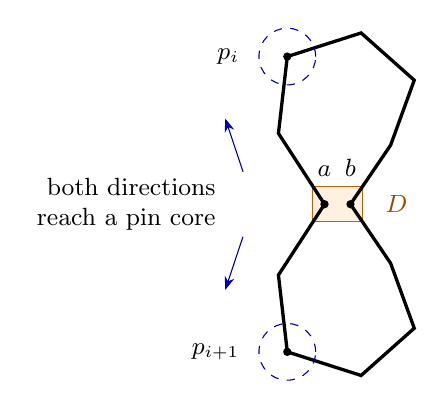
\begin{tikzpicture}[scale=.75,>=Stealth,font=\small]
 \filldraw[fill=orange!12,draw=orange!75!black]
       (-.42,-.3) rectangle (.42,.3);
 \draw[very thick]
       (-.22,0)--(-1,1.2)--(-.85,2.5)--(.4,2.9)
       --(1.3,2.1)--(.9,1.0)--(.22,0)
       --(.9,-1.0)--(1.3,-2.1)--(.4,-2.9)
       --(-.85,-2.5)--(-1,-1.2)--cycle;
 \draw[dashed,blue!70!black] (-.85,2.5) circle (.48);
 \draw[dashed,blue!70!black] (-.85,-2.5) circle (.48);
 \fill (-.22,0) circle (2pt) (.22,0) circle (2pt);
 \fill (-.85,2.5) circle (2pt) (-.85,-2.5) circle (2pt);
 \node[above] at (-.22,.3) {$a$};
 \node[above] at (.22,.3) {$b$};
 \node[right,orange!60!black] at (.65,0) {$D$};
 \node[left] at (-1.5,2.5) {$p_i$};
 \node[left] at (-1.5,-2.5) {$p_{i+1}$};
 \draw[->,blue!70!black] (-1.6,.55)--(-1.9,1.45);
 \draw[->,blue!70!black] (-1.6,-.55)--(-1.9,-1.45);
 \node[left,align=right] at (-1.9,0)
       {both directions\\reach a pin core};
\end{tikzpicture}
\caption{The deterministic implication for a mixed atom $D$, shown in
orange.  The tag $a$
lies on the chunk between consecutive pins $p_i,p_{i+1}$; the other
tag cannot lie on that chunk.  Both intervening rim portions must
therefore reach a distant pin core.  Dashed circles depict the two
cutoffs.  The drawing is schematic and makes no regularity assertion
about a rim.}\label{fig:mixed-atom}
\end{figure}

For sufficiently fine fixed levels, Lemma~\ref{lemma:near-return}
gives the local necessary near-return arm event from scale $O(s_j)$
to a fixed multiple of $h$.  It can be tested inside, for example,
$B(y,10h)$ about the square center $y$, taking the outer radius of
the arm test below $8h$.  The same macroscopically reaching rim
supplies a one-arm event through a separated outer annulus, from
scale $32h$ to a fixed $\delta>0$, whose retained queries can be
confined outside $B(y,24h)$.  The numerical constants can be changed
to fit the fixed buffers.  At fixed $h,j$ the mesh exceptions vanish
and these tests use disjoint deterministic marked-Poisson
restrictions.  For each color $b$, the precise necessary-event
inclusion is
\[
 \begin{aligned}
 &\{\mathcal G;\ \text{atom mixed for some color-}b\text{ rim}\}
 \\
 &\qquad\subset E_{{\rm in},b}(s_j,h)\cap E_{{\rm out},b}(h,\delta)
                 \ \cup\ \{\text{mesh failure}\}.
 \end{aligned}
\]
The events on the right do not select a rim.  We multiply their
ordinary probabilities, not probabilities conditioned on adaptive
labels or on the good event.  The near-return gain and the one-arm
bound give, after decreasing $c>0$ to a common value,
\[
 \PP(E_{{\rm in},b}\cap E_{{\rm out},b})
                         \le C(s_j/h)^{2+c}h^c.
\]
The two colors cost only a factor two.  At the bounded number of
coarse levels where these numerical buffers do not fit, use the
one-arm estimate alone.

On $\mathcal G$, let $N_j$ count the geometric atoms to be considered at level $j$
because their parent is mixed for at least one relevant rim.  At
level zero count the occupied atoms in use.  Each atom is counted
once, regardless of how many rims visit it.  There are
$O_R(s_j^{-2})$ candidate squares, with a bounded number of atoms
and children each. Define $\widehat N_j=\ind_{\mathcal G}N_j$,
with value zero off $\mathcal G$. For $j\ge1$, apply the preceding
inclusion to the mixed parent at scale $s_{j-1}=2s_j$; its bounded
number of children and the factor two in scale change only the
constant. Summing the ordinary arm probabilities yields
\begin{equation}\label{actual:mixed-count}
 \limsup_{\eps\to0}\EE\widehat N_j
                 \le C_Rh^{-2+c}2^{-cj}.
\end{equation}
The same restricted bound at level zero follows from one arm.

Choose $f_D$ to be the value of $f$ at the center of the level-$j$
square containing $D$.  Define the nonnegative square sum
\begin{equation}\label{actual:bessel-level}
 B_j=\sum_{D,\lambda}\left(
       |X_\lambda(\ind_D)|^2+
       s_j^{-2}|X_\lambda(\ind_D(f-f_D))|^2\right).
\end{equation}
The sum includes every deterministic atom at this level and every
circuit-component label $\lambda$.  Since these are disjoint
deterministic masks, $|f-f_D|\le C_fs_j$, and all masks have support
in a fixed compact region, the Bessel bound
\eqref{fields:energy} and the local triangle moments give
\[
              \limsup_{\eps\to0}\EE\widehat B_j\le C_{f,R},
       \qquad \widehat B_j=\ind_{\mathcal H_\eps}B_j.
\]
Here $\mathcal H_\eps$ is the color-independent geometry event of
bulk-patch agreement, and is the whole space in the full-plane setting.
We have $\mathcal G\subset\mathcal H_\eps$. The full deterministic
atom and label sum defining $B_j$ is never restricted according to
the adaptive coefficients; its geometric indicator is allowed in
the conditional Bessel bound.
The bound is uniform in $j$ when that finite level is fixed before
the microscopic limit.

For one rim $P$ let $\mathcal S_j(P)$ be its stopped atoms at
level $j$, and write $\lambda(P)$ for its circuit-component label.
On such an atom its constant coefficient error relative to $f_D$
has magnitude at most $C_fr_h$.  The other error uses $f-f_D$.
Because $s_j\le h\le r_h$, Cauchy--Schwarz gives, on $\mathcal G$,
\begin{align*}
 &\left|\text{level-}j\text{ contribution to }
                    X_P(f)-\mathcal A_X(P)\right|\\
 &\quad\le C_fr_h\sqrt{\#\mathcal S_j(P)}
 \left[\sum_{D\in\mathcal S_j(P)}
       \bigl(|X_{\lambda(P)}(\ind_D)|^2+
       s_j^{-2}|X_{\lambda(P)}(\ind_D(f-f_D))|^2\bigr)\right]^{1/2}\\
 &\quad\le C_fr_h\sqrt{\widehat N_j\widehat B_j}.
\end{align*}
After extending the level error by zero off $\mathcal G$, the last
bound holds everywhere and bounds the maximum over all rims. In particular
no extra number-of-rims factor appears: $\widehat N_j$ counts geometric
atoms, while the second factor already sums over \emph{all} field
labels.  Taking expectation and applying Cauchy--Schwarz once more,
\eqref{actual:mixed-count} and \eqref{actual:bessel-level} bound the
limiting upper expectation by
\[
              C_{f,R}r_hh^{-1+c/2}2^{-cj/2}.
\]
This is summable over levels, with total
$O_{f,R}(r_hh^{-1+c/2})$.

To justify stopping, fix $h$ and a finite depth $J\ge1$. A mixed
level-$J$ atom has a mixed parent for the same rim, so it is itself
counted by $\widehat N_J$ on $\mathcal G$. Therefore
\[
 \limsup_{\eps\to0}
 \PP(\mathcal G\cap\{\text{some level-}J\text{ atom is mixed}\})
                  \le C_Rh^{-2+c}2^{-cJ}.
\]
On $\mathcal G$ when no terminal atom is mixed, the stopped atoms
through depth $J$ account for the whole discrepancy. The preceding
finite sum is bounded by its geometric series, independently of $J$.
For each $t>0$, Markov's inequality and the last display give
\[
 \begin{aligned}
 &\limsup_{\eps\to0}
   \PP\left(\max_P|X_P(f)-\mathcal A_X(P)|>t\right)\\
 &\qquad\le q(h)+C_Rh^{-2+c}2^{-cJ}
                +\frac{C_{f,R}}{t}r_hh^{-1+c/2}.
 \end{aligned}
\]
For a prescribed tolerance $\tau_h\downarrow0$, choose a finite
$J=J(h)$ making the middle term at most $\tau_h$, before taking
$\eps\to0$. Only finitely many mesh tests are needed at that fixed
$h,J$, so their failure terms vanish in this microscopic limit.
Finally let $h\to0$: both $q(h)+\tau_h$ and
$r_hh^{-1+c/2}=h^{c/2-\kappa}$ tend to zero. This proves the claim.
\end{proof}

\subsection{Completion of bulk transport}

Take $\kappa>0$ smaller than half the common positive exponent used
above.  Both terms in \eqref{actual:coefficient-cost} tend to zero,
since they equal, up to constants,
$h^{c-\kappa}(1+|\log h|^2)$ and $h^{c/2-\kappa}$.
Propositions~\ref{prop:dense-pins} and \ref{prop:real-arc}, followed
by Lemma~\ref{lemma:mixed-atoms}, show that for every $\xi>0$,
\begin{equation}\label{actual:ordered-transport}
 \lim_{h\to0}\limsup_{\eps\to0}
 \PP\left(\max_P|Q_P(f)-a_h^QV_P(f)|>\xi\right)=0.
\end{equation}
All limits are on the common microscopic subsequence chosen at the
start of the section.  The auxiliary finite covers and couplings
for a given patch and test require no further subsequence.

Pass along the $h$ sequence so that $a_h^Q\to a\in\C$.
The Bessel bound for $V$ implies
\[
 \limsup_{\eps\to0}
 \PP\left(\max_P|(a_h^Q-a)V_P(f)|>\xi\right)
                         \le C_f|a_h^Q-a|^2/\xi^2.
\]
Combine this with \eqref{actual:ordered-transport}, taking the
microscopic limsup at fixed $h$ and then $h\to0$.  This proves
\eqref{transport:bulk} for the resulting bounded scalar $a$, for
every fixed bulk patch and test $f$.  The scalar choices used only
the countable menu representatives and mean limits, and do not
depend on the later test or on points of evaluation of an observable.
The remaining assertion $\Rea a<1/2$ in
Theorem~\ref{thm:bulk-transport} is established in
Proposition~\ref{prop:nondegeneracy}.

\section{Nondegeneracy of the transport scalar}
\label{sec:nondegeneracy}

Section~\ref{sec:actual-arcs} extracts a limit $a$ of the bounded scalars
$a_h^Q$ and uses the energy bound to obtain \eqref{transport:bulk} with
this single scalar. Its choice depends only on the bulk subsequence, and
does not depend on any probes used in Section~\ref{sec:observable}. We now
prove the asserted restriction on $a$. The strict area imbalance between
the two Fourier fields supplies the positive quantity; contour estimates
and uniform integrability justify passing it through the transport limit.

\begin{proposition}[Nondegeneracy]
\label{prop:nondegeneracy}
Every scalar obtained from the preceding transport construction satisfies
\[
                 1-2\Rea a>0.
\]
In particular, $a\ne1$.
\end{proposition}

Fix a nonzero $f\in C_c^\infty(\C)$ and work in the full plane.
Write $R=Q(f)-aV(f)$. The consequence of bulk transport needed here is
the averaged pairing limit
\begin{equation}
             \EE\langle R,V(f)\rangle\longrightarrow0.
 \label{energy:pairing}
\end{equation}
Here the inner product is in the random label space
$\ell^2(\{\lambda\})$, with the second factor conjugated. Once
\eqref{energy:pairing} is proved, the exact energy identities for $U$ and
$Q$ will force $1-2\Rea a>0$.

Bulk transport gives convergence in probability on macroscopic rims;
it does not by itself justify this sum over all labels or its expectation.
We therefore replace $V(f)$ by contour integrals. Their squared norm on
small rims is negligible, while area multiplicity and wall-count moments
control their macroscopic sum. These two estimates will make the pairing
uniformly integrable and establish \eqref{energy:pairing}.
For a label $\lambda=(L,C)$ with polygonal rim $P$, put
\[
             Y_\lambda=Y_P=\int_P f(z)\,\dd z;
\]
for an isolated-edge component put $Y_\lambda=0$. All rims are oriented as
in Lemma~\ref{lemma:rim}; norms below use the same random label space.

\subsection{Replacing the tagged tangent field by a contour integral}

We first establish the two estimates
\begin{align}
 \EE\sum_\lambda |Y_\lambda-V_\lambda(f)|^2&\longrightarrow0,
 \label{energy:comparison}\\
 \lim_{b\downarrow0}\limsup_{\eps\to0}
 \EE\sum_{\diam(P)<b}|Y_P|^2&=0.
 \label{energy:small-rims}
\end{align}
Choose a compact box $K_0$ containing $\supp f$ in its interior; enlarge it
by a fixed amount whenever a mesh estimate requires a collar.

For a tagged triangle $t$, its clockwise missing side is the corresponding
oriented rim edge. Comparing $f(z_t)$ with $f$ along that edge costs at
most $C_f\diam(t)^2$. An isolated edge has two opposite oriented edge
integrals, which cancel, and the same estimate applies to its two tags.
Consequently there are nonnegative budgets
\[
 B_\lambda=C_f\!\sum_{\substack{t\text{ tagged by }\lambda\\
                         t\cap\supp f\ne\varnothing}}
                         \diam(t)^2
 \quad\text{such that}\quad
 |Y_\lambda-V_\lambda(f)|\le B_\lambda.
\]
Triangles in a vanishing mesh collar may be included in this sum without
changing the argument. A triangle has at most one tag, so
$S_\eps=\sum_\lambda B_\lambda$ has uniformly bounded moments of every
fixed finite order by Lemma~\ref{lemma:mesh}.

We claim that $M_\eps=\max_\lambda B_\lambda\to0$ in probability.
First fix $b>0$ and tile a neighborhood of $\supp f$ by squares of side
$s\ll b$. If a rim of diameter at least $b$ has a tag in such a square,
then, on fine mesh, its monochromatic path gives an arm from a fixed
enlargement of the square to distance of order $b$. The local
diameter-square sum has $L^2$ norm at most $Cs^2$ in the microscopic upper
limit. Cauchy--Schwarz and the one-arm estimate therefore bound the
expected budget in that square belonging to these rims by
\[
                    C_f s^2(s/b)^{c/2}
\]
in that upper limit. There are $O(s^{-2})$ squares. Thus the total budget
of the rims of diameter at least $b$ vanishes in probability after first
taking $\eps\to0$ and then $s\downarrow0$.

A rim of diameter less than $b$ has all its relevant tags in an enlarged
box of side $O(b)$ on fine mesh. The same is true of an isolated tag pair.
Cover the fixed support neighborhood by $O(b^{-2})$ such boxes. If $D_B$
denotes the diameter-square sum in an enlarged box, then, for every fixed
$p>1$,
\[
 \limsup_{\eps\to0}\PP\!\left(\max_B D_B>u\right)
 \le C_p u^{-p}b^{2p-2},\qquad u>0,
\]
using the local $L^p$ bound $\limsup_{\eps\to0}\|D_B\|_p\le C_pb^2$.
Letting $b\downarrow0$ proves the claim. Finally,
\[
 \sum_\lambda |Y_\lambda-V_\lambda(f)|^2
       \le M_\eps S_\eps.
\]
The right side tends to zero in probability and is uniformly integrable:
$M_\eps\le S_\eps$ and the latter has bounded moments of order greater
than two. This proves \eqref{energy:comparison}.

\subsection{Distinct walls and area multiplicity}

We need two bounds on these contours: a small-diameter estimate for
their expected square sum, and higher moments of their absolute sum
above a fixed diameter cutoff. Both follow by counting distinct walls
and controlling how many of one wall's component interiors cover a point.

Stokes' theorem, applied with either orientation, gives
\begin{equation}
 |Y_P|\le C_f\int_{K_0}\ind_{\operatorname{int}_b(P)}(z)\,\dd^2z,
 \label{energy:stokes}
\end{equation}
where $\operatorname{int}_b(P)$ is the bounded geometric inside of $P$.
Also, $Y_P=0$ unless $P$ meets $K_0$.

For each fixed wall $L$, at most two of its rims enclose a generic point.
Indeed, the bounded components of the untouched triangles have disjoint
disk interiors by Lemma~\ref{lemma:rim}; in addition, there is only one
unbounded component. Its rim can contribute one further bounded inside.
Polygonal boundaries have area zero, so this pointwise assertion is
sufficient for all area integrals below. It is an area-multiplicity
statement, and does not bound the number of rims associated with a wall.

We record the wall-count estimate used at both small and fixed scales.
At any scale $t>0$, the expected number of rims of diameter in $[t,2t]$
enclosing a specified generic point is bounded uniformly in $t$ and
$\eps$. Such a rim lies within distance $2t$ of the point. On mesh fine
relative to $t$, its wall visits the triangles facing the rim edges and
therefore has a spanning arc in one of finitely many fixed-ratio annuli
centered at a grid of mesh a small fixed multiple of $t$. Nested primal
boundary cycles with room between them may be chosen as in
Section~\ref{sec:probability}. For each such annulus, let $N$ count the
proper spanning wall strands obtained by cutting at all boundary
contacts and stopping at the boundary edges. Use the bank extraction
from the proof of Lemma~\ref{lemma:mixed-four}: every strand has an
adjacent black bank, each gap between consecutive strands accounts for
at most two such banks, and banks selected from distinct gaps give
vertex-disjoint black crossings after proper trimming. This includes
their boundary endpoints, by the stopped-edge argument in that proof:
each black boundary site belongs to only one gap.
In particular, $N\ge2k$ supplies $k$ crossings with
disjoint site witnesses. On the crossing-good geometry event $G$, a
fixed buffered subannulus has quenched white-circuit probability at
least $\delta>0$, supplied by finitely many fixed-aspect rectangle tests.
Such a circuit excludes a black spanning crossing. BK, applied
conditionally on the point geometry, therefore gives
\[
            \Peta(N\ge2k)\le(1-\delta)^k\qquad\text{on }G.
\]
Consequently the spanning-strand counts have bounded quenched moments
of every fixed order on $G$.

Here and below the exceptional geometry is controlled quantitatively.
For $t/\eps$ large, the probability that either the needed mesh or crossing
tests fail is at most $C_\gamma(t/\eps)^{-\gamma}$, for any prescribed
finite $\gamma$, by Proposition~\ref{prop:probability-input} and
Lemma~\ref{lemma:mesh}. Without these tests, count distinct walls by the
number $J$ of incident triangles in the relevant $O(t)$ region. Every
counted wall has a tagged incident triangle there, and the moments of $J$
grow at most polynomially in $1+t/\eps$. For example, if
\[
 \|J\|_{2m}\le C(1+t/\eps)^{k_m},
\]
then
\[
 \EE[J^m\ind_{\mathrm{bad}}]
 \le \|J\|_{2m}^{m}\PP(\mathrm{bad})^{1/2}
 \le C(1+t/\eps)^{mk_m}(t/\eps)^{-\gamma/2}.
\]
Choose $\gamma>2mk_m$. For bounded $t/\eps$, the incidence bound alone
suffices. The two-per-wall area multiplicity gives the asserted uniform
expected rim count.

Since $|Y_P|\le C_ft^2$ for $\diam(P)\in[t,2t]$, this count and
\eqref{energy:stokes} imply
\[
 \EE\sum_{t\le\diam(P)<2t}|Y_P|^2
 \le C_ft^2\int_{K_0}
       \EE\sum_{t\le\diam(P)<2t}
            \ind_{\operatorname{int}_b(P)}(z)\,\dd^2z
 \le C_f t^2.
\]
Dyadic summation over scales below $b$ proves
\eqref{energy:small-rims}.

For fixed $b>0$, let $N_{\eps,b}$ count the distinct walls represented by
rims with $\diam(P)\ge b$ and $Y_P\ne0$. Cover $K_0$ by finitely many grid
balls whose radii are a sufficiently small fixed fraction of $b$. A rim
of diameter at least $b$ meeting one of these balls must leave a fixed
enlargement of it, so its wall has a spanning arc in a corresponding
fixed-ratio annulus. The preceding spanning-arc and bad-geometry estimates,
now at fixed scale, prove
\[
          \sup_{\eps\text{ small}}\EE N_{\eps,b}^{m}<\infty
          \qquad (b>0,\ m<\infty).
\]
The constants may depend on $b$ and $m$. Put $M_f=C_f\Area(K_0)$.
Applying area multiplicity before summing labels gives the precise bounds
\begin{align}
 \sum_{\diam(P)\ge b}|Y_P|&\le 2M_fN_{\eps,b},\notag\\
 \sum_{\diam(P)\ge b}|Y_P|^2&\le 2M_f^2N_{\eps,b}.
 \label{energy:macro-multiplicity}
\end{align}
In the second line we used $|Y_P|\le M_f$ individually. Thus the absolute
sum, and the square sum, have all fixed higher moments at fixed $b$,
without a count of all rims belonging to one wall.

\subsection{Uniform integrability and the positive area identity}

Put $A_\eps=\|R\|_{\ell^2}$.
The energy identity gives $\sup_\eps\|A_\eps\|_2<\infty$.
At fixed $b$, split $f$ into finitely many smooth tests supported on disks
small compared with $b$. Every relevant rim leaves the fourfold disk of
each such test that it meets. Hence \eqref{transport:bulk} gives
\[
 \delta_{\eps,b}:=\max_{\substack{\diam(P)\ge b\\Y_P\ne0}}
                           |R_P|\longrightarrow0
 \quad\text{in probability}.
\]
By \eqref{energy:macro-multiplicity},
\[
 \left|\sum_{\diam(P)\ge b}R_P\overline{Y_P}\right|
 \le\delta_{\eps,b}\sum_{\diam(P)\ge b}|Y_P|
 \longrightarrow0
 \quad\text{in probability}.
\]
For the required passage to expectation, define
$B_{\eps,b}=(\sum_{\diam(P)\ge b}|Y_P|^2)^{1/2}$.
For any fixed $q>2$ the wall moments give
$\sup_\eps\|B_{\eps,b}\|_q<\infty$. With
$p=2q/(q+2)>1$, Cauchy--Schwarz in labels and H\"older in probability give
\begin{equation}
 \left\|\sum_{\diam(P)\ge b}R_P\overline{Y_P}\right\|_p
 \le\|A_\eps B_{\eps,b}\|_p
 \le\|A_\eps\|_2\|B_{\eps,b}\|_q\le C_{b,f}.
 \label{energy:macro-ui}
\end{equation}
This is uniform integrability, so the macroscopic pairing tends to zero
in $L^1$. The two errors left in replacing this pairing by the full
pairing with $V(f)$ satisfy
\begin{align*}
 \EE|\langle R,V(f)-Y\rangle|
 &\le (\EE\|R\|^2)^{1/2}
            (\EE\|V(f)-Y\|^2)^{1/2},\\
 \EE\left|\sum_{\diam(P)<b}R_P\overline{Y_P}\right|
 &\le (\EE\|R\|^2)^{1/2}
       \left(\EE\sum_{\diam(P)<b}|Y_P|^2\right)^{1/2}.
\end{align*}
The first vanishes as $\eps\to0$ by \eqref{energy:comparison}; the second
vanishes after the microscopic upper limit and then $b\downarrow0$ by
\eqref{energy:small-rims}. This proves the pairing limit
\eqref{energy:pairing}.

\begin{proof}[Proof of Proposition~\ref{prop:nondegeneracy}]
Since $V=U+Q$, the cross terms in the following real part cancel exactly.
By \eqref{fields:energy} and the triangle area identity,
\begin{align*}
 \EE\Re\sum_\lambda(V_\lambda(f)-2Q_\lambda(f))
                                      \overline{V_\lambda(f)}
 &=\EE\sum_\lambda\bigl(|U_\lambda(f)|^2-|Q_\lambda(f)|^2\bigr)\\
 &=\sqrt3\,\EE\sum_t\Area(t)|f(z_t)|^2
 \longrightarrow\sqrt3\int_\C|f(z)|^2\,\dd^2z>0.
\end{align*}
The final approximation follows from fine mesh and the diameter moments.
On the other hand, \eqref{energy:pairing} writes the left side as
\[
              (1-2\Rea a)\,\EE\|V(f)\|^2+o(1).
\]
The norm is nonnegative and has bounded expectation. A nonpositive
coefficient is incompatible with the strictly positive limit. Therefore
$1-2\Rea a>0$, as claimed.
\end{proof}

\section{The observable and the crossing limit}
\label{sec:observable}

We construct an observable with a boundary coefficient equal to the
desired crossing probability, and use bulk transport to prove that its
limit is holomorphic.

We first identify the free crossing limit on disks approximating a
polygonal Jordan quadrilateral. We then compare those crossings with the
closed-cell event in an arbitrary Jordan domain. All random discrete
domains in this section are chosen from the point geometry, independently
of the colors.

\subsection{Discrete disks and the closing star}

\begin{lemma}[Ordered polygonal approximation]
\label{lemma:polygonal-disks}
Let $D$ be a polygonal Jordan domain with finitely many marked boundary
points in their cyclic order. With probability tending to one, the
Delaunay triangulation contains a simple primal cycle whose boundary and
selected marked vertices converge to the marked boundary of $D$ in order
and in Fr\'echet distance. The triangulation inside this cycle agrees with
the full-plane triangulation on every fixed compact subset of $D$ for
all sufficiently fine good approximations.
\end{lemma}

\begin{proof}
On fine mesh in a fixed collar of $\partial D$, record the successive
Voronoi cell sites met during one traversal of $\partial D$ and join
successive sites by primal edges. A fixed polygon meets cell switches
generically almost surely. Equivalently, one can use walks through the
nearby triangles. This produces a closed primal walk, with sites and
edges uniformly close to the boundary position at the corresponding
traversal times. Its winding about a fixed interior point is one.

Extract return loops and contract them to obtain the oriented
simple-cycle decomposition of this walk. Winding is additive, so retain
a cycle with positive winding about the interior point, retaining the
original cyclic times of its edges. Every dropped interval of times has
endpoints whose physical positions tend together. Boundary simplicity
then forces its parameter length to tend to zero, unless it tends to a
whole turn. The latter possibility would put all retained times, and
thus the retained cycle, in a shrinking neighborhood of one boundary
point, contradicting its positive winding about the fixed interior
point. Hence the retained cycle follows the boundary in its order, and
marked vertices can be selected at the desired parameters. Finite
deterministic tie-breaking makes the choice measurable. Filling the
cycle by its interior triangles gives the required disk. The mesh and
local-determination estimates ensure agreement on interior compacts.
Taking a deterministic sequence of decreasing tolerances gives the
claimed convergence in probability.
\end{proof}

Fix such a disk, and initially retain only the three marked vertices
$v_0,v_1,v_2$ approximating $a,c,d$, respectively, in positive order.
Indices in the fan construction are taken modulo three. Add an exterior
vertex $s_i$ fanned to the inclusive boundary arc $v_i v_{i+1}$, add the
junction triangles $s_{i-1}s_i v_i$, and close the exterior by a triangle
$t_*$ with vertices $s_0,s_1,s_2$. This is a simple triangulation of the
sphere. Give the added vertices independent fair colors, as for the
original disk sites. No Euclidean weights on the exterior triangles are
needed.

At the closing star $t_*$, let $n_i$ be a point on the dual spoke crossing
$s_{i-1}s_i$, and assign it the label $w_i=\om^i$. This order is
\emph{opposite} to the positive cyclic order at $t_*$. For a probe $m$ in
the interior of a dual edge, define, conditionally on the geometry $\eta$,
\begin{equation}
 F_m^\eta=4\sum_{i=0}^2w_iK(m,n_i)
          =4\Esp\bigl[w_*H_{\lambda_*}(m)\bigr].
 \label{observable:definition}
\end{equation}
In the second expression, if $t_*$ is occupied by an ordinary wall, let
$i$ be its missing port and let $\lambda_*$ be that wall together with
the component reached through the missing port; set $w_*=w_i$. Set the
entire contribution to zero if $t_*$ is unused. To verify the equality,
observe that a wall not using $t_*$ has identical component indicators at
all three $n_i$, and its contribution is killed by $\sum_iw_i=0$.
The observable is constant along the interior of a dual edge, so we also
write $F_e^\eta$ for its value at a primal edge $e$. In the physical disk
the dual probe can be chosen at the intersection with that side.

Figure~\ref{fig:closing-fans} shows the completion and the boundary
pairing used below. The kernel definition is adapted to orthogonality;
its alternative description as a mean partner label will give positivity
and identify the crossing coefficient.

\begin{figure}[htbp]
\centering
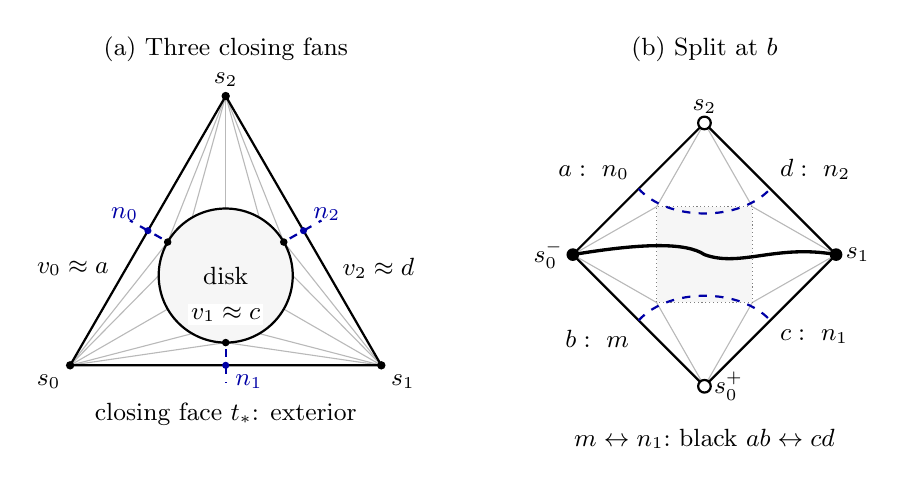
\begin{tikzpicture}[scale=.76, every node/.style={font=\small}]
\begin{scope}
 \coordinate (s0) at (-2.6,-1.5);
 \coordinate (s1) at (2.6,-1.5);
 \coordinate (s2) at (0,3);
 \fill[gray!7] (0,0) circle (1.12);
 \foreach \ang in {150,180,210,240,270}
   \draw[gray!55] (s0)--(\ang:1.12);
 \foreach \ang in {270,300,330,360,390}
   \draw[gray!55] (s1)--(\ang:1.12);
 \foreach \ang in {30,60,90,120,150}
   \draw[gray!55] (s2)--(\ang:1.12);
 \draw[thick] (s0)--(s1)--(s2)--cycle;
 \draw[thick] (0,0) circle (1.12);
 \foreach \pos in {150,270,30}{
   \fill (\pos:1.12) circle (1.8pt);
 }
 \node[anchor=east,fill=white,inner sep=1pt] at (-1.9,.12) {$v_0\approx a$};
 \node[fill=white,inner sep=1pt] at (0,-.65) {$v_1\approx c$};
 \node[anchor=west,fill=white,inner sep=1pt] at (1.9,.12) {$v_2\approx d$};
 \fill (s0) circle (2pt) node[below left] {$s_0$};
 \fill (s1) circle (2pt) node[below right] {$s_1$};
 \fill (s2) circle (2pt) node[above] {$s_2$};
 \node at (0,0) {disk};
 \draw[blue!65!black,dashed,thick] (-1.07,.62)--(-1.60,.92);
 \draw[blue!65!black,dashed,thick] (0,-1.23)--(0,-1.80);
 \draw[blue!65!black,dashed,thick] (1.07,.62)--(1.60,.92);
 \fill[blue!65!black] (-1.3,.75) circle (1.7pt)
   node[above left] {$n_0$};
 \fill[blue!65!black] (0,-1.5) circle (1.7pt)
   node[below right] {$n_1$};
 \fill[blue!65!black] (1.3,.75) circle (1.7pt)
   node[above right] {$n_2$};
 \node[align=center] at (0,-2.32) {closing face $t_*$\text{: exterior}};
 \node at (0,3.78) {(a) Three closing fans};
\end{scope}
\begin{scope}[xshift=8.0cm,yshift=.35cm]
 \coordinate (l) at (-2.2,0);
 \coordinate (r) at (2.2,0);
 \coordinate (u) at (0,2.2);
 \coordinate (v) at (0,-2.2);
 \fill[gray!7] (-.8,-.8) rectangle (.8,.8);
 \draw[gray!55] (l)--(-.8,.8) (l)--(-.8,-.8)
   (v)--(-.8,-.8) (v)--(.8,-.8)
   (r)--(.8,-.8) (r)--(.8,.8)
   (u)--(.8,.8) (u)--(-.8,.8);
 \draw[thick] (l)--(v)--(r)--(u)--cycle;
 \draw[gray,densely dotted] (-.8,-.8) rectangle (.8,.8);
 \draw[very thick] (l) .. controls (-1,.20) and (-.3,.20) .. (0,0)
    .. controls (.6,-.22) and (1.2,.18) .. (r);
 \draw[blue!65!black,dashed,thick] (-1.1,-1.1)
    .. controls (-.6,-.55) and (.6,-.55) .. (1.1,-1.1);
 \draw[blue!65!black,dashed,thick] (-1.1,1.1)
    .. controls (-.6,.55) and (.6,.55) .. (1.1,1.1);
 \foreach \p in {l,r} \fill (\p) circle (3pt);
 \foreach \p in {u,v} \draw[fill=white,thick] (\p) circle (3pt);
 \node[left] at (l) {$s_0^-$};
 \node[right] at (r) {$s_1$};
 \node[above] at (u) {$s_2$};
 \node[right] at (v) {$s_0^+$};
 \node[above left] at (-1.1,1.1) {$a:\ n_0$};
 \node[below left] at (-1.1,-1.1) {$b:\ m$};
 \node[below right] at (1.1,-1.1) {$c:\ n_1$};
 \node[above right] at (1.1,1.1) {$d:\ n_2$};
 \node[align=center] at (0,-3.08) {$m\leftrightarrow n_1$:\ black $ab\leftrightarrow cd$};
 \node at (0,3.43) {(b) Split at $b$};
\end{scope}
\end{tikzpicture}
\caption{The closing construction and one of the two boundary pairings.
In (a), the unbounded face of the drawing is the closing triangle on the
sphere; the dashed segments indicate its dual spokes. Thus the labels
$n_0,n_1,n_2$ run opposite to the positive order at its dual star.
In (b), splitting $s_0$ produces black fans on $ab,cd$ and white fans on
$bc,da$. The labels indicate the attachments of the four boundary
switches. Dashed strands show the pairing $m$--$n_1$, $n_0$--$n_2$;
the solid black path shows the corresponding connection of the black
fans. In (b), only the exterior colors are prescribed; all original disk
vertices remain free. The drawings are topological schematics.}
\label{fig:closing-fans}
\end{figure}

\par\ifdim\dimexpr\pagegoal-\pagetotal\relax<6\baselineskip\newpage\fi
\begin{proposition}[Triangular observable and the crossing coefficient]
\label{prop:observable}
The value $F_m^\eta$ belongs to the closed triangle with vertices
$w_0,w_1,w_2$. At a fan probe $s_i u$, where $u$ is interior to the boundary
arc $v_i v_{i+1}$, it belongs to the side $[w_i,w_{i+1}]$. For $i=0$ and
$u$ the marked vertex approximating $b$, the coefficient of $w_1$ on this
side is exactly the free black vertex crossing probability between the
arcs approximating $ab$ and $cd$ in the original disk.
\end{proposition}

\begin{proof}
Start with the uniform edge-pattern ensemble having oddness at $t_*$ and
$m$, and move the star defect to $n_i$ as in the proof of
\eqref{fields:orthogonal}. If the star has degree one, the loop count is
independent of the chosen port. If it has degree three, the extra loop
count is the indicator that the exterior partner of $m$ is port $i$:
joining the other two star ports creates exactly that extra loop.
Degree three has probability $1/4$. Indeed, toggling a fixed defect path
bijects to the even ensemble, whose four local even patterns at the star
are equiprobable. The port-independent terms cancel in the weighted
sum, and the factor four in \eqref{observable:definition} cancels this
probability. Thus $F_m^\eta$ is the mean partner label conditional on
degree three, proving the triangular convex-combination assertion.

For a fan probe $s_i u$, split $s_i$ into two exterior vertices, fanned
respectively to the two successive subarcs, both containing $u$, and add
the triangle formed by these two vertices and $u$. Remove $t_*$ and
prescribe alternating colors, in one fixed convention, on the four
exterior vertices now present. Leave all original disk spins free. The
four boundary edges joining consecutive exterior vertices are switches.
Their disagreement strands have the preceding conditional pairing law.

Here is the parity correspondence explicitly. The two half-edge values
at the old probe, with oddness there, have exactly one occupied half.
They become the two spoke values entering the added triangle, which has
even parity because its split exterior boundary edge is occupied. The
other three occupied exterior boundary edges are the three forced
switches at the old degree-three star. This gives a bijection from the
conditional edge-pattern ensemble to parity-even disagreement data on
all triangles of the augmented disk, with the four boundary switches
fixed. Triangle parity gives cycle parity, so the data recover colors up
to a global flip. Fixing the alternating exterior convention removes
that flip, leaving exactly uniform independent colors on all original
disk vertices.

The four switches have a noncrossing pairing. The split switch can
therefore be paired only with port $i$ or port $i+1$, proving the side
constraint. For $i=0$ at $u\approx b$, prescribe the exterior vertices
along $ab$ and $cd$ to be black, and the other two to be white. Connecting
the two black exterior vertices is equivalent to a black crossing in the
original disk: any connection between the two black fans contains a path
of original black vertices between their respective arcs, and conversely
such a path joins the fans. Pairing the split switch with port $1$ gives
this connection along the neighboring black sites. The other pairing
joins the opposite white pair, and the two possibilities are exclusive
by planarity. This proves the stated coefficient identity.
\end{proof}

\subsection{Annealed compactness for geometry-selected probes}

On failed disk-approximation events, extend all observables by arbitrary
bounded values. Those events have vanishing probability and will not
affect a limit. Original disk spins are always coupled to the fair
full-plane site colors.

The admissible probes in this subsection and below are original disk
edges, located at their physical midpoints, and fan edges $s_i u$,
located at their disk attachments $u$. A geometry-selected probe tends
to a fixed point when its location converges in probability to that
point.

\begin{lemma}[Probe compactness]
\label{lemma:probe-compactness}
From every microscopic sequence one can select a subsequence, still
satisfying the bulk transport conclusion, on which the annealed
observables converge to a continuous function $F$ in $D$ and on its three
open boundary arcs. The convergence holds for every geometry-measurable
choice of admissible probes tending to a specified point off the three
marks. The limit takes values in the closed triangle and has the
corresponding closed side values on the
open boundary arcs.
\end{lemma}

\begin{proof}
We use the ordinary-wall representation in
\eqref{observable:definition}. A nonisolated selected component has a rim
using the exterior edge $s_{i-1}s_i$, followed by a path of original disk
sites between attachments to the two different boundary arcs of those
fans. The third exterior vertex has the opposite color and cannot lie on
this rim. The disk path can degenerate to the common endpoint of its two
arcs. The component indicator tests the component side of the rim,
including its rim edges: an open dual edge belongs to that component
exactly when it is incident to an untouched triangle on the filled disk
side. An isolated selected component contributes zero at the probes in
use.

For two nearby bulk probes, different indicators force a selected-rim
visit between them. Such a visit gives a monochromatic path of original
disk sites from their neighborhood to a fixed positive distance, since
the disk portion reaches the boundary. Near a boundary point off the
three marks, compare a fan probe first with its attached disk vertex.
Unless that vertex lies on the rim, following its incident fan edge to
the vertex tests the same side; if it does lie on the rim, the required
visit already occurs. Uniform closed-disk Jordan charts join nearby disk
positions tending to the same boundary point by paths of vanishing
diameter inside the closed approximating disk. Thus a difference again
forces a nearby visit by the disk portion of the selected rim. Its two
attachments lie on different marked arcs and cannot both approach this
nonmark boundary point. One direction of the disk path therefore reaches
a fixed positive distance \emph{among original disk sites}. The exterior
fan edges do not replace this arm.

More precisely, on a fixed compact set off the marks choose a positive
distance $\rho$ valid for these continuations. For probes in a small
neighborhood of diameter $s$, choose a deterministic enlarged
neighborhood containing their short comparison paths on good geometry.
Let $q_{s,\rho}(\eta)$ be the conditional probability of a monochromatic
arm of either color from that neighborhood to distance $\rho$, under the
full-plane independent site colors. Then, for every pair of admissible
geometry-selected probes in that neighborhood, the same test gives
\begin{equation}
             |F_m^\eta-F_{m'}^\eta|
                    \le4q_{s,\rho}(\eta).
 \label{observable:conditional-arm}
\end{equation}
There is no union bound over the chosen edges. The disk and chart control
needed for this statement follows along every deterministic sequence of
good marked Jordan approximations by closed Jordan convergence; mesh
control transfers edges to their sites. Taking expectations and using
the ordinary one-arm estimate gives an upper limit tending to zero as
$s\downarrow0$. The geometry errors vanish first at fixed $s$.

Choose near-position representative edges at a countable dense set of
interior points, and fan representatives at a countable dense set of each
open boundary arc. These choices exist with vanishing location error on
good geometry. Boundedness permits a diagonal subsequence of their
annealed expectations. Estimate~\eqref{observable:conditional-arm}
extends the resulting function continuously and identifies the same
limit for all geometry-selected probes converging to any such point.
The triangle and side constraints pass to this limit by
Proposition~\ref{prop:observable}. All choices are made after the
universal bulk subsequence, so the transport conclusions remain valid.
\end{proof}

\subsection{Holomorphy without separating geometry and colors}

\begin{proposition}[Holomorphy]
\label{prop:holomorphy}
Every limit $F$ in Lemma~\ref{lemma:probe-compactness} is holomorphic in
$D$.
\end{proposition}

\begin{proof}
For a smooth compactly supported bulk test $f$, orthogonality against the
closing star, with its reversed labels, gives the exact conditional
identity
\[
                 \Esp[w_*U_{\lambda_*}(f)]=0.
\]
Indeed, at every bulk triangle the weighted sum
$\sum_j\om^jF_{m_j(t)}^\eta$ is zero by
\eqref{fields:orthogonal}. The selected nonisolated rim reaches the
exterior and therefore leaves every sufficiently small fixed test
collar. An isolated selected pair tags only exterior triangles. Apply
\eqref{transport:bulk}, partitioning $f$ into local disk tests when
needed. Its residual at the selected label tends to zero in probability
and in mean: its absolute value is bounded by the full residual
$\ell^2$ norm, which is bounded in $L^2$ by \eqref{fields:energy}.
Since
\[
 U=(1-a)V-(Q-aV),\qquad a\ne1,
\]
we obtain $\EE[w_*V_{\lambda_*}(f)]\to0$. On high-probability geometry
events the discrete disk agrees with the full triangulation throughout
the test collars; the conditional identities hold on each such graph.
The energy moments remove the omitted geometry.

Using \eqref{observable:definition} and $\sum_jd_{tj}=0$, we have therefore
proved
\begin{equation}
 \EE\left[\sum_t f(z_t)\sum_jd_{tj}F_{m_j(t)}^\eta\right]
                          \longrightarrow0.
 \label{observable:discrete-cr}
\end{equation}
The edge coefficients and the conditional observable both depend on the
point geometry, so their product cannot be replaced by a product of
expectations. We instead express the edge coefficients as a random
measure and prove that this measure has a deterministic limit.

Group the two contributions of each shared edge $e=t\cap t'$. If $d_{t,e}$
is its clockwise side vector for $t$, set
\[
 \mu_\eps=\sum_e d_{t,e}\bigl(f(z_t)-f(z_{t'})\bigr)\delta_{m_e},
\]
where now $m_e$ denotes the physical midpoint of the side. This weight is
independent of which adjacent triangle is called $t$. All edges involved
are buffered inside the disk. Let $T_\eps(B)=|\mu_\eps|(B)$.
Because $f$ is smooth,
\[
 |d_{t,e}|\,|f(z_t)-f(z_{t'})|
 \le C_f\bigl(\diam(t)^2+\diam(t')^2\bigr).
\]
Consequently, for each sufficiently small fixed square $B$ of side $s$
in a compact bulk neighborhood,
\begin{equation}
        \limsup_{\eps\to0}\|T_\eps(B)\|_2\le C_fs^2.
 \label{observable:variation}
\end{equation}
The triangles incident to an edge assigned to $B$ lie in a fixed
enlargement on fine mesh; the exceptional contribution is controlled by
their higher moments.

For a deterministic smooth function $G$, midpoint integration on
clockwise triangle boundaries gives
\[
 \mu_\eps(G)
 \longrightarrow -\int_D f\,\dd G\wedge\dd z
              =\int_DG\,\dd f\wedge\dd z
                 \quad\text{in }L^1\text{ of the geometry}.
\]
To check the approximation, the midpoint error on a triangle is
$O_{f,G}(\diam(t)^3)$. The sum of these errors tends to zero in $L^1$,
using the maximum mesh diameter times the bounded diameter-square sum.
Stokes' theorem, the clockwise orientation, and area approximation give
the displayed sign. Replacing $f(z_t)$ by $f$ in each triangle has the
same vanishing cubic-error bound. The resulting limiting complex measure
is
\[
                     \mu=\dd f\wedge\dd z,
\]
which has a bounded compactly supported density.

We need the stronger conclusion for fixed-square indicators. If $B$ is
such a square, choose a smooth $g_\tau$ with $0\le g_\tau\le1$ agreeing
with $\ind_B$ outside a boundary strip $U_\tau$ of width $O(\tau)$. Then
\[
 |\mu_\eps(B)-\mu(B)|
 \le |\mu_\eps(g_\tau)-\mu(g_\tau)|
                   +T_\eps(U_\tau)+|\mu|(U_\tau).
\]
Cover $U_\tau$ by $O(\operatorname{perimeter}(B)/\tau+1)$ squares of
side $O(\tau)$. The first-moment consequence of
\eqref{observable:variation}, after the microscopic limit, makes the
expected variation on this strip $O_f(\operatorname{perimeter}(B)\tau+
\tau^2)$. The limiting variation tends to zero there as well. First take
$\eps\to0$, then $\tau\downarrow0$, obtaining
\begin{equation}
                W_\eps(B):=\mu_\eps(B)\longrightarrow
                w(B):=\mu(B)\quad\text{in }L^1.
 \label{observable:square-l1}
\end{equation}

Now fix a deterministic tiling of the test neighborhood by squares of
side $s$, and choose a conditional representative $F_B^\eta$ on an edge
near the center of each square. The same ordinary arm test in
\eqref{observable:conditional-arm} controls every edge assigned to $B$:
\[
 |F_e^\eta-F_B^\eta|\le4q_B(\eta),\qquad
 \limsup_{\eps\to0}\EE q_B\le C(s/\rho)^c,
 \qquad 0\le q_B\le1.
\]
Here $\rho>0$ is fixed by the distance of the support neighborhood to the
boundary. Thus $\EE q_B^2\le\EE q_B$, and without an independence
assumption Cauchy--Schwarz gives
\[
 \limsup_{\eps\to0}\EE[T_\eps(B)q_B]
      \le C_{f,\rho}s^{2+c/2}.
\]
Summing over $O(s^{-2})$ squares bounds the mean replacement error by
$C_{f,\rho}s^{c/2}$. For fixed $s$, omitted geometry contributes a
vanishing mean by boundedness of the observable and the variation
moments.

At this fixed tiling, \eqref{observable:square-l1} can be multiplied by
the correlated representative because $|F_B^\eta|\le1$:
\[
 \left|\EE[F_B^\eta W_\eps(B)]-w(B)\EE F_B^\eta\right|
 \le\EE|W_\eps(B)-w(B)|\longrightarrow0.
\]
Lemma~\ref{lemma:probe-compactness} identifies
$\EE F_B^\eta\to F(\operatorname{center}(B))$. Hence
\eqref{observable:discrete-cr}, followed first by $\eps\to0$ at fixed
tiling and then by $s\downarrow0$, yields
\begin{equation}
                       \int_D F\,\dd f\wedge\dd z=0
                       \qquad(f\in C_c^\infty(D)).
 \label{observable:cr}
\end{equation}
Since $\dd f\wedge\dd z=2\ii\,\partial_{\bar z}f\,\dd^2z$, this is
the distributional Cauchy--Riemann equation. Local mollification and
continuity of $F$ show that $F$ is holomorphic.
\end{proof}

\subsection{The three boundary arcs determine the conformal map}

The three closed sides of a nondegenerate triangle have empty common
intersection. The side constraints therefore show that $F$ is
nonconstant. The open mapping theorem puts its interior values in the
open equilateral triangle. Conformal charts for the polygon and the
triangle, with their Carath\'eodory boundary extensions, reduce the
remaining uniqueness issue to the following lemma.

\par\ifdim\dimexpr\pagegoal-\pagetotal\relax<6\baselineskip\newpage\fi
\begin{lemma}[Boundary uniqueness]
\label{lemma:boundary-uniqueness}
Let $G:\mathbb D\to\mathbb D$ be nonconstant and holomorphic. Let
$\zeta_0,\zeta_1,\zeta_2$ and $\eta_0,\eta_1,\eta_2$ be positively
ordered triples of distinct points of the unit circle. Suppose that $G$
extends continuously to each open arc $(\zeta_i,\zeta_{i+1})$ and takes
its values there in the corresponding positively oriented closed arc
$[\eta_i,\eta_{i+1}]$. Then $G$ extends continuously to the closed disk,
maps $\zeta_i$ to $\eta_i$, and is a conformal bijection of the disk.
\end{lemma}

\begin{proof}
On each open source arc, Schwarz reflection across the unit circle
extends $G$ holomorphically across the boundary. Near each point of that
arc, $G$ is nonzero, so $u=\log|G|$ is harmonic, negative on the disk
side, and zero on the circle. The Hopf boundary lemma and the
Cauchy--Riemann equations give
\[
 \frac{\dd}{\dd t}\arg G(e^{\ii t})
    =\left.\frac{\partial}{\partial r}\log|G(re^{\ii t})|\right|_{r=1}
    >0.
\]
The proper target arc has a bounded real argument lift. Thus the
boundary argument on each open source arc is strictly increasing and
has finite one-sided limits at its endpoints.

We prove that the two limits at a source mark agree, without assuming
interior continuity there. Rotate that mark to $1$ and denote the limits
as $t\uparrow0$ and $t\downarrow0$ by $L_-$ and $L_+$, respectively.
Let $g(e^{\ii t})$ be the known boundary values, with arbitrary values
assigned at the three marks. For fixed $z\in\mathbb D$, Cauchy's formula
on a circle of radius $R>|z|$ is
\[
 G(z)=\frac1{2\pi}\int_{-\pi}^{\pi}
       \frac{G(Re^{\ii t})}{1-(z/R)e^{-\ii t}}\,\dd t.
\]
As $R\uparrow1$, the numerator converges away from the three marks and
is uniformly bounded, while the denominator stays uniformly away from
zero for this fixed $z$. Dominated convergence therefore gives
\[
 G(r)=\frac1{2\pi}\int_{-\pi}^{\pi}
                 \frac{g(e^{\ii t})}{1-re^{-\ii t}}\,\dd t,
                 \qquad 0<r<1.
\]
For a fixed small $\alpha>0$, write $\ell_r=\log(1/(1-r))$. The
logarithmic primitive of the kernel gives
\[
 \int_0^\alpha\frac{\dd t}{1-re^{-\ii t}}
       =\frac{\ell_r}{\ii}+O_\alpha(1),\qquad
 \int_{-\alpha}^0\frac{\dd t}{1-re^{-\ii t}}
       =-\frac{\ell_r}{\ii}+O_\alpha(1).
\]
For example, a continuous branch of
$\ii^{-1}\log(e^{\ii t}-r)$ is a primitive on either interval.
Moreover, the kernel is bounded in modulus by
$C/(1-r+|t|)$ there. Replacing $g$ by its corresponding one-sided
limit therefore gives an $o(\ell_r)$ error: for every $\delta>0$ choose
a smaller fixed interval where $|g-L_\pm|<\delta$, use the logarithmic
kernel bound on that interval, and note that the complementary fixed
interval has a bounded integral as $r\uparrow1$. Then let $\delta$ tend
to zero. The part away from the mark is also bounded. Consequently,
\begin{equation}
 G(r)=\frac{L_+-L_-}{2\pi\ii}\log\frac1{1-r}
            +o\!\left(\log\frac1{1-r}\right).
 \label{observable:jump}
\end{equation}
Boundedness of $G$ forces $L_+=L_-$. The common value belongs to the two
adjacent target arcs, whose intersection is their prescribed common
endpoint; hence $G$ has the required continuous circle trace $g$.

To obtain continuity for all interior approaches, apply the same
radial-circle limiting argument to the Poisson formula for the bounded
harmonic real and imaginary parts of $G$. They are the Poisson
extensions of the continuous circle trace $g$. The Poisson extension of
continuous circle data is continuous on the closed disk. In particular,
this proves full continuity at the marks, not merely radial or
nontangential convergence.

On each open arc the boundary argument increases strictly between the
two prescribed consecutive endpoints. The boundary curve therefore
traverses the circle once in positive order. For any $w\in\mathbb D$,
continuity on the closed disk gives uniform convergence of
$G(re^{\ii t})-w$ to $g(e^{\ii t})-w$ as $r\uparrow1$. The winding number
is one for all sufficiently large $r$. The argument principle gives
exactly one zero of $G-w$ in $|z|<r$, counted with multiplicity. Letting
$r\uparrow1$ proves that every $w$ has exactly one preimage, of
multiplicity one. Thus $G$ is a conformal bijection.
\end{proof}

It follows that $F$ is the conformal map to the equilateral triangle with
$a,c,d$ mapped to $w_0,w_1,w_2$. Normalize a conformal map to the upper
half-plane by
\[
                  (a,b,c,d)\longmapsto(0,x,1,\infty),\qquad 0<x<1.
\]
The Schwarz--Christoffel integral for three angles $\pi/3$ gives the
proportion along the side from $w_0$ to $w_1$ at $b$ as
\begin{equation}
 \mathcal C(x)=
 \frac{\displaystyle\int_0^x u^{-2/3}(1-u)^{-2/3}\,\dd u}
      {\displaystyle\int_0^1 u^{-2/3}(1-u)^{-2/3}\,\dd u}.
 \label{observable:beta}
\end{equation}
By Proposition~\ref{prop:observable}, this is the limiting annealed
coefficient of $w_1$ at the fan probe for $b$, and therefore the limiting
free black vertex crossing probability. Every microscopic sequence has
a further subsequence with this same limit. Since the crossing
probabilities are bounded, their full sequence converges to
$\mathcal C(x)$ on the discrete polygonal disks.

\subsection{The closed-cell event in every Jordan domain}

\begin{proposition}[Fixed-buffer Jordan comparison]
\label{prop:jordan-squeeze}
Let $D$ be any bounded Jordan domain with distinct positively ordered
boundary marks $a,b,c,d$. For the full-plane Poisson tessellation with
independent fair cell colors, the annealed probability of a connected
crossing in the closed black-cell union intersected with $\overline D$,
from $ab$ to $cd$, converges to $\mathcal C(x)$ with the marked conformal
parameter of $D$.
\end{proposition}

\begin{proof}
Choose an orientation-preserving plane Jordan--Schoenflies homeomorphism
$\Phi$ taking $\overline D$ to $[0,1]^2$, with the target arcs $ab$ and
$cd$ going to the left and right sides. For fixed $0<\delta<1/8$, define
in these coordinates the harder and easier rectangles
\[
 R^-_\delta=[-\delta,1+\delta]\times[\delta,1-\delta],
 \qquad
 R^+_\delta=[\delta,1-\delta]\times[-\delta,1+\delta].
\]
The first rectangle lengthens a horizontal crossing while restricting
its height; the second shortens the crossing and allows more height.
Figure~\ref{fig:jordan-buffers} displays these two comparisons.
Approximate their inverse images under $\Phi$ by deterministic polygonal
marked quadrilaterals, in their boundary order and much more accurately
than the buffer margins. For each of the two polygons use the discrete
disks from Lemma~\ref{lemma:polygonal-disks}. Their original vertices
inherit the full-plane free colors, so the crossing results already
proved apply to them.

\begin{figure}[htbp]
\centering
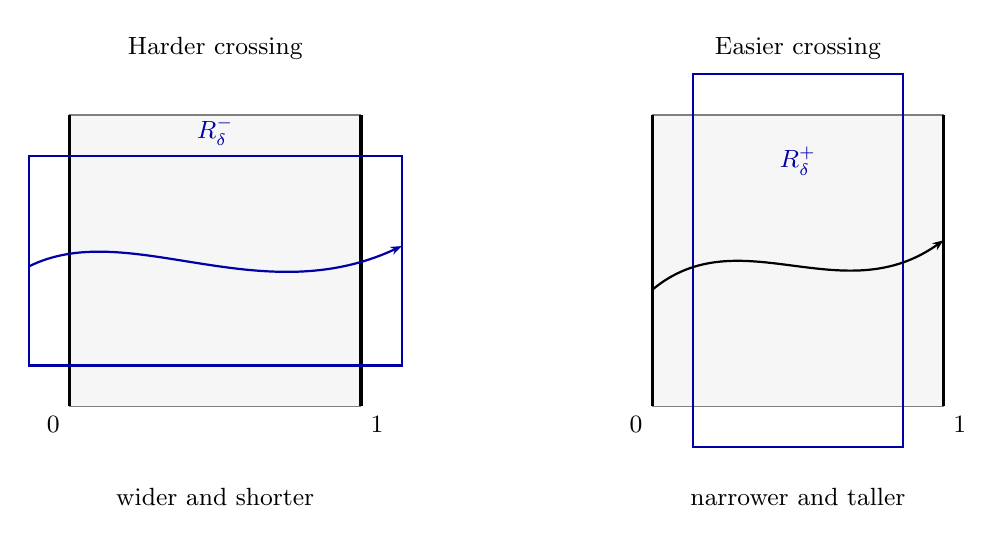
\begin{tikzpicture}[scale=3.7,every node/.style={font=\small}]
 \begin{scope}
  \fill[gray!7] (0,0) rectangle (1,1);
  \draw[gray] (0,0) rectangle (1,1);
  \draw[very thick] (0,0)--(0,1) (1,0)--(1,1);
  \draw[blue!65!black,thick] (-.14,.14) rectangle (1.14,.86);
  \draw[blue!65!black,thick,-{Stealth[length=4pt]}]
    (-.14,.48) .. controls (.20,.65) and (.65,.32) .. (1.14,.55);
  \node[below left] at (0,0) {$0$};
  \node[below right] at (1,0) {$1$};
  \node[blue!65!black,above] at (.5,.86) {$R^-_\delta$};
  \node at (.5,1.23) {Harder crossing};
  \node[align=center] at (.5,-.31) {wider and shorter};
 \end{scope}
 \begin{scope}[xshift=2.0cm]
  \fill[gray!7] (0,0) rectangle (1,1);
  \draw[gray] (0,0) rectangle (1,1);
  \draw[very thick] (0,0)--(0,1) (1,0)--(1,1);
  \draw[blue!65!black,thick] (.14,-.14) rectangle (.86,1.14);
  \draw[thick,-{Stealth[length=4pt]}]
    (0,.40) .. controls (.30,.65) and (.65,.32) .. (1,.57);
  \node[below left] at (0,0) {$0$};
  \node[below right] at (1,0) {$1$};
  \node[blue!65!black,above] at (.5,.76) {$R^+_\delta$};
  \node at (.5,1.23) {Easier crossing};
  \node[align=center] at (.5,-.31) {narrower and taller};
 \end{scope}
\end{tikzpicture}
\caption{Fixed buffers in the coordinates of $\Phi$. The gray square is
$\Phi(\overline D)$, with its two target sides in bold; the blue boundary
is the comparison rectangle. A path crossing the harder rectangle
contains a crossing of the square, while a path crossing the square
contains a crossing of the easier rectangle. Strict margins preserve
these implications under the
polygonal and discrete approximations. The picture is in square
coordinates and imposes no metric regularity on the physical Jordan
boundary or on the chart.}
\label{fig:jordan-buffers}
\end{figure}

Keep all these choices fixed while taking $\eps\to0$. Work on the
high-probability event of the needed disk approximation and mesh control
in a fixed compact neighborhood. Both $\Phi$ and $\Phi^{-1}$ are uniformly
continuous on the relevant compact sets. Thus any fixed coordinate
margin is preserved by taking the physical polygonal and mesh errors
sufficiently small. No Lipschitz estimate for either chart is required.

\paragraph{The harder crossing implies a closed-cell crossing.}
A black primal vertex crossing of the harder disk gives a continuous
black-cell path: for each successive pair of neighboring sites, join
them through their shared Voronoi side, with the two segments lying in
the two closed black cells. Mesh control keeps this path uniformly close
to the primal path. In square coordinates it stays in a height band
strictly inside $(0,1)$, starts to the left of $x=0$, and ends to the
right of $x=1$. Take its first contact with $x=1$ and the last preceding
contact with $x=0$. Between those times its first coordinate lies in
$[0,1]$, and its height remains in $(0,1)$. This clipped path is therefore
a crossing of $\overline D$ in the closed black-cell union.

\paragraph{A connected closed-cell crossing gives a finite primal chain.}
First recall local finiteness, including cells whose nuclei lie outside
the region of interest. On a fixed compact neighborhood, the distance
to the nearest site has a finite maximum: a finite cover, or comparison
with any fixed site, gives such a bound. A cell meeting that neighborhood
has its nucleus within the resulting bounded enlargement. Poisson local
finiteness therefore leaves only finitely many such cells.

If a connected crossing set is not closed, take its closure. The black
cell union is closed locally, being a locally finite union of closed
cells. The closure consequently remains black, connected, and contained
in $\overline D$, and retains its contacts with both target arcs. Denote
this compact connected set by $K$. For every black cell $C_j$ meeting
$K$, let $E_j=K\cap C_j$. These finitely many nonempty relatively closed
sets cover $K$. Their incidence graph is connected: a partition into two
nonempty collections with no intersecting members would express $K$ as
the disjoint union of two relatively closed sets, a separation. Hence
there is a finite touching chain of black cells from a left-contact cell
to a right-contact cell.

Cells meeting along a Voronoi edge have neighboring sites. If two cells
meet only at a Voronoi vertex, Poisson general position gives exactly
three cells there, with nuclei forming a Delaunay triangle; those two
sites are again neighbors. Thus the touching chain yields a black
full-plane primal vertex chain, also for the vertex-only contacts
permitted by the closed-cell event. Fine mesh makes its nuclei and edges
arbitrarily close to $K$. For an edge of the chain, use its cell-contact
point in $K$: both neighboring nuclei lie close to that point, and so
does their straight Delaunay edge. This justifies the proximity without
any convexity assumption on $D$.

\paragraph{The chain contains a crossing of the easier disk.}
In square coordinates the chain stays in a small enlargement of
$[0,1]^2$, starts strictly to the left of the easier disk, and ends
strictly to its right. Its allowed height band is disjoint from the
easier disk's entire top and bottom boundary arcs. A fixed vertical
middle strip within that band lies inside the approximating disk; its
left and right boundary-arc neighborhoods lie on opposite sides of this
strip. These assertions have strict margins, so hold for the polygonal
and discrete approximations already fixed.

\begingroup\widowpenalty=10000
The chain and the disk boundary are paths in the same planar primal
graph. They can meet only at vertices or along shared edges. The chain
has a left boundary contact before its first right boundary contact:
to reach the right side from its starting position it must pass through
the interior middle strip, and the top and bottom arcs are inaccessible.
Choose that first right contact, and then the last left contact
preceding it. Between these contacts there are no boundary visits.
Any shared boundary edge would have boundary endpoint vertices and
would also be such a visit. The intervening subpath crosses the interior
middle strip, since its endpoints lie on opposite sides. A connected
path avoiding a simple boundary cycle cannot move between its interior
and exterior. This subpath is therefore in the interior, with its two
endpoints on the left and right vertex arcs of the closed disk. Removing
repeated vertices if necessary gives its black crossing.\par
\endgroup

\paragraph{Limit order.}
Write $p^-_{\eps,\delta}$ and $p^+_{\eps,\delta}$ for the free crossing
probabilities of these fixed harder and easier discrete disks, and
$p_\eps(D;a,b,c,d)$ for the requested closed-cell probability. The two
pathwise comparisons, with the vanishing geometry exception, imply
\[
 p^-_{\eps,\delta}-o(1)
 \le p_\eps(D;a,b,c,d)
 \le p^+_{\eps,\delta}+o(1),
\]
where $\delta$ and the deterministic polygons are fixed during the
microscopic limit. The outer probabilities converge to
$\mathcal C(x^-_\delta)$ and $\mathcal C(x^+_\delta)$ by the polygonal
result. Now shrink the buffers, choosing their polygonal approximation
errors to vanish faster than their coordinate margins. The marked
boundaries converge in order and in Fr\'echet distance to the original
Jordan boundary. Closed Jordan conformal convergence gives
$x^-_\delta,x^+_\delta\to x$. Since $\mathcal C$ is continuous on
$(0,1)$, the displayed inequalities squeeze the requested limit to
$\mathcal C(x)$.
\end{proof}

Finally,
\[
 \int_0^1u^{-2/3}(1-u)^{-2/3}\,\dd u
             =\frac{\Gamma(1/3)^2}{\Gamma(2/3)},\qquad
 \int_0^xu^{-2/3}(1-u)^{-2/3}\,\dd u
             =3x^{1/3}\,{}_2F_1(1/3,2/3;4/3;x).
\]
The second identity follows by integrating the binomial series on
$[0,x]$, and $\Gamma(4/3)=\Gamma(1/3)/3$. Substitution into
\eqref{observable:beta} yields exactly \eqref{eq:cardy}. Together with
Proposition~\ref{prop:jordan-squeeze}, this proves
Theorem~\ref{thm:cardy} for the stated full-plane annealed law and the
closed-cell convention.

\bibliographystyle{plain}
\bibliography{references}
\end{document}
